\documentclass[a4paper,12pt]{report}

\usepackage[romanian]{babel}
\usepackage[a4paper,top=2cm,bottom=2cm,left=3cm,right=3cm,marginparwidth=1.75cm]{geometry}
\usepackage[colorlinks=true, allcolors=black]{hyperref}
\usepackage[nottoc,numbib]{tocbibind}
\usepackage{amsmath}
\usepackage{graphicx}
\usepackage{indentfirst}
\usepackage{enumitem}
\usepackage{placeins}
\usepackage{fontspec}
\usepackage{longtable}
\usepackage{array}

\setlength{\parindent}{5mm}
\setlength{\parskip}{6pt}

\setmainfont{UTSans}[
    Path=./fonts/,
    Extension = .ttf,
    UprightFont=*-Regular,
    BoldFont=*-Bold,
    ItalicFont=*-Regular,
    ItalicFeatures={FakeSlant=0.25}
]

\begin{document}

\begin{titlepage}
    \begin{center}
        \begin{minipage}{8cm}
            
\includegraphics[width=\linewidth]{images/unitbv.jpg}
        \end{minipage}
        \hfill
        \begin{minipage}{5cm}
            \textbf{Programul de studiu:}\\
            Informatică
        \end{minipage}
    \end{center}

    \vspace{3cm}

    \begin{center}
        \textbf{\LARGE Lucrare de licență}\\
        \vspace{0.5cm}
        \textbf{\Large Sistem de gestionare al accesului într-o parcare auto folosind tehnici de procesare a imaginilor}\\
        \vspace{2cm}
        \textbf{Autor: George Daniel Patrașc}\\
        \textbf{Coordonator științific: Lect. Dr. Honorius Cezar Gâlmeanu}\\
        \vspace{2cm}
        \textbf{Brașov, 2024}
    \end{center}
\end{titlepage}

\tableofcontents

\chapter{Introducere}
\section{Scopul aplicației}
Aplicația are scopul de a facilita și automatiza gestionarea accesului în parcările auto, prin identificarea și înregistrarea automată a numerelor de înmatriculare ale autovehiculelor, aducând beneficii eficienței operaționale și securității.

\begin{figure}[h!]
    \centering
    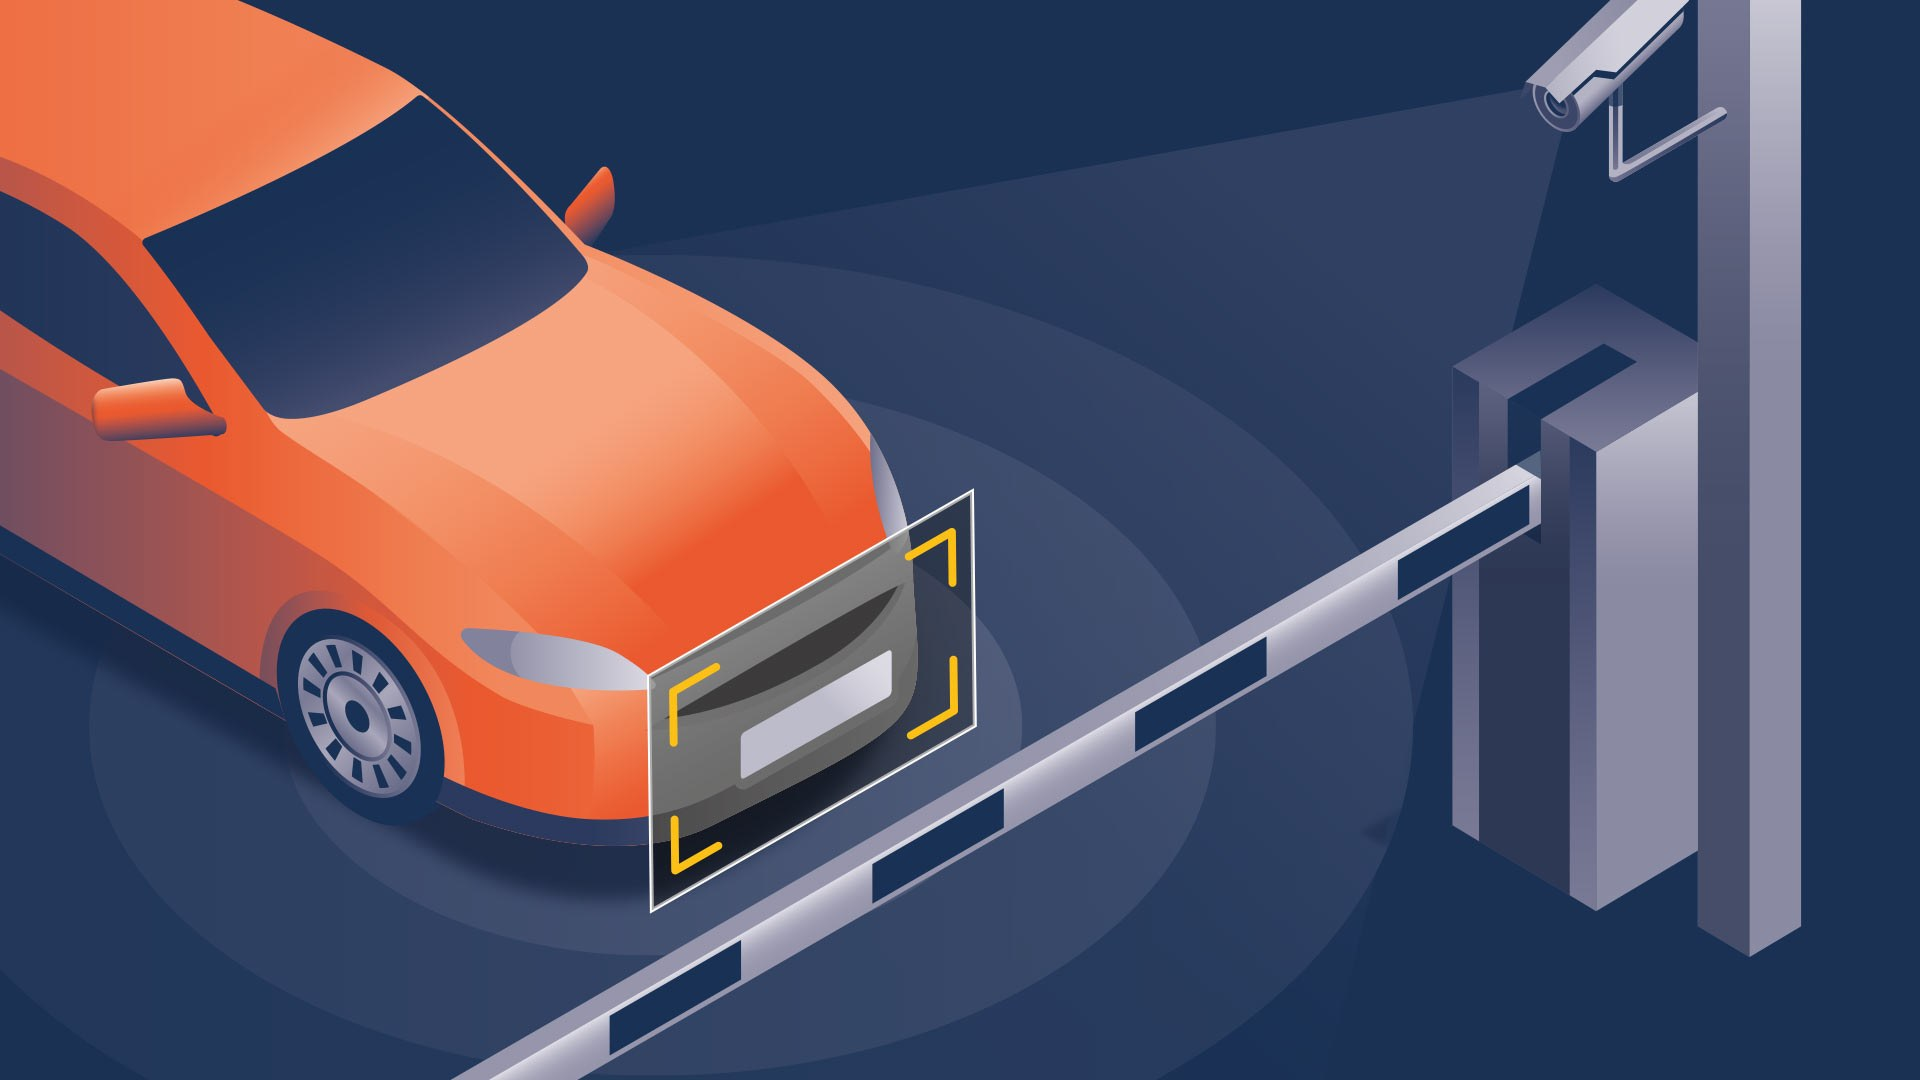
\includegraphics[width=0.7\textwidth]{images/picture.jpg}
\end{figure}
\FloatBarrier

\begin{enumerate}[label=\Roman*.]
    \item \textbf{Detectarea și identificarea automată a numărului de înmatriculare:} Aplicația utilizează camere video poziționate strategic pentru a capta imagini ale vehiculelor la momentul intrării sau ieșirii acestora din parcare. Aceste imagini sunt analizate în timp real pentru a se detecta și recunoaște numerele de înmatriculare.
    \item \textbf{Prelucrarea imaginilor:} Folosind algoritmi de procesare a imaginilor și tehnici de segmentare, aplicația extrage și rectifică numărul de înmatriculare din imaginea captată, asigurându-se că textul este clar în imagine.
    \item \textbf{Recunoașterea textului prin tehnologii de inteligență artificială:} Odată ce numărul de înmatriculare este izolat și optimizat, modelul AI Tesseract de recunoaștere optică a caracterelor (OCR) interpretează textul. Acest model este antrenat să recunoască în special fonturile și stilurile numerelor de înmatriculare.
    \item \textbf{Înregistrarea și monitorizarea accesului:} Numerele de înmatriculare recunoscute sunt înregistrate într-o bază de date. Aceasta permite urmărirea vehiculelor care intră și ies din parcare, oferind date importante pentru securitate și gestionarea spațiului de parcare.
    \item \textbf{Interfața grafică de utilizator (GUI):} Aplicația include o interfață grafică prietenoasă și intuitivă, care afișează în timp real informațiile despre accesul în parcare. Interfața permite utilizatorilor să vizualizeze imagini recente și să acceseze istoricul vehiculelor care au pătruns în parcare.
\end{enumerate}

\section{Motivarea aplicației}
În cadrul proiectului, s-a urmărit dezvoltarea unei soluții eficiente prin valorificarea cunoștințelor existente din domeniul procesării imaginilor. Totodata, proiectul a implicat aplicarea și extinderea tehnicilor de analiză și procesare vizuală, pentru a identifica și extrage numerele de înmatriculare din imaginile captate de la intrările în parcările auto.

Ca limbaj de programare s-a optat pentru C++, care este larg recunoscut în domeniul procesării de imagini datorită eficienței sale remarcabile și a flexibilității pe care o oferă în gestionarea resurselor de sistem, contribuind la optimizarea timpului de execuție si permițând manipularea avansată și rapidă a datelor vizuale.

Pe parcursul dezvoltării soluției, s-a pus accent pe integrarea unei suite de tehnologii și instrumente de dezvoltare pentru a optimiza atât procesul de elaborare, cât și performanța finală a sistemului. În acest sens, s-a utilizat biblioteca OpenCV, care a fost esențială în lucrul cu imagini si utilizarea algoritmilor de procesare. De asemenea, s-a folosit modelul de inteligență artificială Tesseract OCR, recunoscut pentru eficiența sa în recunoașterea optică a caracterelor, pentru a extrage textul clar și precis din imagini.

Interfața grafică a fost creată cu ajutorul framework-ului Qt, oferind o manieră eficientă de interacțiune și o vizualizare intuitivă a datelor procesate. Pentru managementul proiectului și automatizarea construcției sistemului, s-au folosit CMake și Doxygen, acesta din urmă facilitând generarea documentației tehnice detaliate. De asemenea, pentru a asigura robustețea codului, s-au implementat unit teste, care au permis verificarea și validarea funcționalităților în diverse scenarii de utilizare.

Întregul proces de dezvoltare a fost suportat de mediul integrat de dezvoltare Visual Studio, și a fost gestionat folosind GitLab pentru versionarea codului.

\chapter{Noțiuni teoretice}
\section{Ce este imaginea digitală si procesarea de imagine?}
O imagine poate fi definită ca o funcție bidimensională, f$(x,y)$, unde x și y sunt coordonate spațiale, iar amplitudinea lui f la orice pereche de coordonate $(x, y)$ este numită intensitatea sau nivelul de gri al imaginii în acel punct. Când x, y și valorile intensității lui f sunt finite și discrete, imaginea se numește imagine digitală. Procesarea imaginii digitale se referă la procesarea imaginilor digitale cu ajutorul unui computer digital. O imagine digitală este compusă dintr-un număr finit de elemente, fiecare având o locație și o valoare specifică, numite pixeli.

Viziunea este cel mai avansat simț al nostru, astfel încât imaginile joacă un rol esențial în percepția umană. Spre deosebire de oameni, care sunt limitați la spectrul vizual al radiațiilor electromagnetice, mașinile de imagistică acoperă aproape întregul spectru electromagnetic, de la raze gamma la unde radio. Acestea pot opera pe imagini generate de surse neobișnuite pentru oameni, cum ar fi ultrasunetele, microscopie electronică și imagini generate de computer.

Nu există un acord general privind granițele dintre procesarea imaginii, analiza imaginii și viziunea computerizată. Uneori, procesarea imaginii este definită ca o disciplină în care atât intrarea, cât și ieșirea sunt imagini. Aceasta poate fi o definiție limitativă. Pe de altă parte, viziunea computerizată are ca scop imitarea vederii umane, inclusiv învățarea și luarea deciziilor pe baza inputurilor vizuale, fiind o ramură a inteligenței artificiale.

Un exemplu de procesare a imaginii digitale este analiza automată a textului, care include achiziția imaginii, preprocesarea, extragerea și recunoașterea caracterelor individuale. Înțelegerea conținutului paginii poate fi considerată analiză a imaginii sau chiar viziune computerizată, în funcție de complexitate.

\section{Spații de culoare}
În procesarea imaginilor, spațiile de culoare sunt modalități de a reprezenta culorile în modele numerice care facilitează manipularea și analiza imaginilor. Cele mai comune spații de culoare utilizate sunt Grayscale, RGB și HSV.

Grayscale (tonuri de gri) este un spațiu de culoare în care fiecare pixel este reprezentat de o singură valoare care indică intensitatea luminii. Valorile sunt de obicei cuprinse între 0 (negru) și 255 (alb) pentru imagini pe 8 biți. Conversia unei imagini color într-o imagine grayscale se face prin combinarea componentelor de culoare ale fiecărui pixel într-o singură valoare de luminanță.

\begin{figure}[h!]
    \centering
    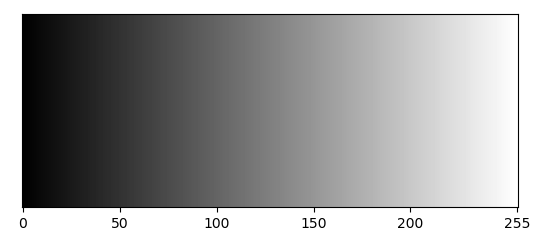
\includegraphics[width=0.5\textwidth]{images/grayscale.jpg}
    \caption{Gradientul Grayscale}
\end{figure}
\FloatBarrier

RGB (Red, Green, Blue) este un spațiu de culoare aditiv în care orice culoare poate fi creată prin combinarea celor trei culori primare: roșu, verde și albastru. Fiecare componentă are o valoare între 0 și 255 într-o imagine pe 8 biți.

\begin{figure}[h!]
    \centering
    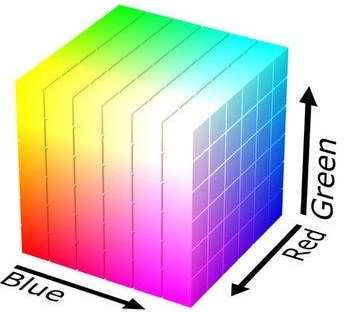
\includegraphics[width=0.5\textwidth]{images/RGB.jpg}
    \caption{Cubul RGB}
\end{figure}
\FloatBarrier

HSV (Hue, Saturation, Value) este un spațiu de culoare care reprezintă culoarea într-un mod mai intuitiv pentru percepția umană. Cele trei componente sunt:
\begin{itemize}
    \item \textbf{Hue (nuanță)}: descrie tipul de culoare și este măsurat în grade de la 0 la 360.
    \item \textbf{Saturation (saturație)}: descrie intensitatea culorii și variază de la 0 (gri) la 1 (culoare pură).
    \item \textbf{Value (valoare)}: descrie luminozitatea culorii și variază de la 0 (negru) la 1 (alb complet).
\end{itemize}

\begin{figure}[h!]
    \centering
    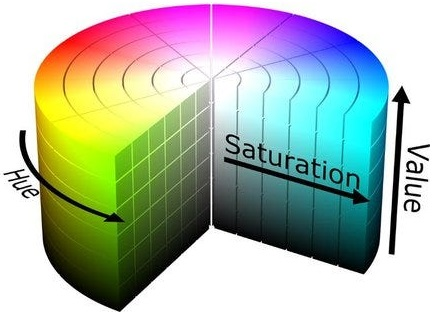
\includegraphics[width=0.5\textwidth]{images/HSV.jpg}
    \caption{Cilindrul HSV}
\end{figure}
\FloatBarrier

Conversia între diferite spații de culoare este adesea necesară în procesarea imaginilor pentru a facilita anumite operații. Aceste conversii permit adaptarea și prelucrarea imaginilor în funcție de cerințele specifice ale aplicațiilor, fie că este vorba de îmbunătățirea contrastului, identificarea obiectelor sau alte tehnici de analiză. Iată câteva formule de bază pentru conversie:
\begin{enumerate}
    \item \textbf{Conversia RGB la Grayscale}:
          \[
              Y = 0.299 \cdot R + 0.587 \cdot G + 0.114 \cdot B
          \]
          Această formulă folosește o combinație ponderată a componentelor roșu, verde și albastru pentru a calcula luminanța, rezultând o imagine în tonuri de gri care păstrează percepția de lumină a imaginii originale.

    \item \textbf{Conversia RGB la HSV}:
          \[
              C_{\max} = \max(R, G, B)
          \]
          \[
              C_{\min} = \min(R, G, B)
          \]
          \[
              \Delta = C_{\max} - C_{\min}
          \]

          \[
              H = \begin{cases}
                  0                                                               & \text{dacă } \Delta = 0   \\
                  60^\circ \times \frac{G - B}{\Delta} + 360^\circ \mod 360^\circ & \text{dacă } C_{\max} = R \\
                  60^\circ \times \frac{B - R}{\Delta} + 120^\circ                & \text{dacă } C_{\max} = G \\
                  60^\circ \times \frac{R - G}{\Delta} + 240^\circ                & \text{dacă } C_{\max} = B
              \end{cases}
          \]

          \[
              S = \begin{cases}
                  0                       & \text{dacă } C_{\max} = 0 \\
                  \frac{\Delta}{C_{\max}} & \text{altfel}
              \end{cases}
          \]

          \[
              V = C_{\max}
          \]

          Conversia RGB la HSV este utilă deoarece spațiul HSV este mai intuitiv pentru percepția umană a culorilor, facilitând operații cum ar fi ajustarea saturației sau a nuanței fără a afecta celelalte componente de culoare.

    \item \textbf{Conversia HSV la RGB}:
          \[
              C = V \times S
          \]
          \[
              X = C \times (1 - \left| \left(\frac{H}{60^\circ} \mod 2 \right) - 1 \right|)
          \]
          \[
              m = V - C
          \]

          \[
              (R, G, B) = \begin{cases}
                  (C+m, X+m, m) & \text{dacă } 0 \leq H < 60^\circ          \\
                  (X+m, C+m, m) & \text{dacă } 60^\circ \leq H < 120^\circ  \\
                  (m, C+m, X+m) & \text{dacă } 120^\circ \leq H < 180^\circ \\
                  (m, X+m, C+m) & \text{dacă } 180^\circ \leq H < 240^\circ \\
                  (X+m, m, C+m) & \text{dacă } 240^\circ \leq H < 300^\circ \\
                  (C+m, m, X+m) & \text{dacă } 300^\circ \leq H < 360^\circ
              \end{cases}
          \]

          Această conversie permite transformarea din spațiul de culoare HSV în RGB, ceea ce este util pentru afișarea imaginilor după ce au fost manipulate în spațiul HSV. Conversiile între aceste spații de culoare permit efectuarea de prelucrări complexe pe imagini, cum ar fi filtrarea bazată pe nuanță sau saturație, care sunt greu de realizat direct în spațiul RGB.
\end{enumerate}

\section{Histograma}
Să notăm cu $r_k$, pentru $k = 0, 1, 2, \ldots, L-1$, intensitățile unei imagini digitale de nivel $L$, $f(x, y)$. Histograma ne-normalizată a lui $f$ este definită ca:
\[
    h(r_k) = n_k \quad \text{pentru } k = 0, 1, 2, \ldots, L-1
\]
unde $n_k$ este numărul de pixeli din $f$ cu intensitatea $r_k$, iar subdiviziunile scalei de intensitate sunt numite \textit{bin-uri de histogramă}. În mod similar, histograma normalizată a lui $f$ este definită ca:
\[
    p(r_k) = \frac{h(r_k)}{MN} = \frac{n_k}{MN}
\]
unde, ca de obicei, $M$ și $N$ sunt numărul de rânduri și coloane ale imaginii, respectiv. În general, lucrăm cu histograme normalizate, la care ne referim simplu ca histogramă sau histograme de imagine. Suma valorilor $p(r_k)$ pentru toate valorile lui $k$ este întotdeauna 1. Componentele $p(r_k)$ sunt estimări ale probabilităților de apariție a nivelurilor de intensitate într-o imagine.

Forma histogramei este legată de apariția imaginii. De exemplu, presupunem imagini cu patru caracteristici de bază ale intensității: întunecată, luminoasă, contrast scăzut și contrast ridicat. Într-o imaginea întunecată, cele mai populate bin-uri ale histogramei sunt concentrate la capătul inferior (mai întunecat) al scalei de intensitate. Similar, majoritatea pixelilor luminoși sunt concentrați spre capătul superior al scalei de intensitate. O imagine cu contrast scăzut are o histogramă îngustă situată de obicei în jurul mijlocului scalei de intensitate. Pentru o imagine monocromă, aceasta implică un aspect gri, plictisitor.

Într-o imagine cu contrast ridicat, componentele histogramei acoperă un interval larg al scalei de intensitate, iar distribuția pixelilor nu este prea departe de uniformă, doar câteva bin-uri fiind mult mai înalte decât altele. Intuitiv, este rezonabil să concluzionăm că o imagine ale cărei pixeli tind să ocupe întregul interval de niveluri de intensitate posibile și, în plus, tind să fie distribuiți uniform, va avea un aspect de contrast ridicat și va prezenta o mare varietate de tonuri de gri. Efectul net va fi o imagine care arată o mare cantitate de detalii de nivel gri și are un interval dinamic ridicat.

\section{Decupare și redimensionare}
Decuparea este o operațiune esențială în prelucrarea imaginilor care presupune selecționarea unei subzone dintr-o imagine și eliminarea restului. Aceasta este utilă pentru focalizarea pe o regiune de interes specifică, eliminarea zonelor nedorite sau pregătirea imaginii pentru analize ulterioare. Procesul de decupare implică specificarea unui dreptunghi delimitat de coordonatele colțului din stânga sus (x, y) și dimensiunile lățimii (w) și înălțimii (h).

Redimensionarea unei imagini implică schimbarea dimensiunilor acesteia pentru a se potrivi unor specificații date. Acest proces este esențial în diverse aplicații, cum ar fi pregătirea imaginilor pentru rețele neurale, ajustarea pentru afișare pe ecrane de diferite dimensiuni sau pregătirea pentru imprimare.

Pentru a redimensiona o imagine, trebuie să specificăm dimensiunea dorită a imaginii rezultate. Aceasta poate fi realizată în două moduri:
\begin{itemize}
    \item \textbf{Redimensionare absolută}: Dimensiunea dorită a imaginii de ieșire este setată direct prin specificarea lățimii și înălțimii.
    \item \textbf{Redimensionare relativă}: Dimensiunea imaginii de ieșire este determinată prin factori de scalare aplicați axelor x și y.
\end{itemize}

Un aspect important al redimensionării este metoda de interpolare utilizată pentru a calcula valorile pixelilor în imaginea redimensionată. Metodele comune de interpolare includ:
\begin{itemize}
    \item \textbf{Interpolare cea mai apropiată}: Valoarea pixelului redimensionat este luată de la cel mai apropiat pixel din imaginea sursă.
    \item \textbf{Interpolare biliniară}: Valorile a patru pixeli din vecinătatea pixelului redimensionat sunt ponderate linear în funcție de distanța lor față de pixelul de destinație.
    \item \textbf{Interpolare bicubică}: Se utilizează o spline cubică pentru a interpola valorile dintr-o zonă 4x4 din jurul pixelului redimensionat.
    \item \textbf{Interpolare Lanczos}: Utilizează o funcție sinc trunchiată pentru a interpola valorile dintr-o zonă 8x8 din jurul pixelului redimensionat.
\end{itemize}

Metoda de interpolare influențează calitatea imaginii redimensionate, cu metode mai sofisticate oferind de obicei rezultate mai netede și mai precise, dar la un cost computațional mai mare.

\section{Padding}
Corelația produce un rezultat care este mai mic decât imaginea originală, ceea ce poate să nu fie de dorit în multe aplicații. Aceasta se datorează faptului că vecinătățile corelației tipice și operațiile de convoluție se extind dincolo de limitele imaginii în apropierea marginilor, astfel încât imaginile filtrate suferă de efecte de bordură (boundary effects).

Pentru a rezolva această problemă, au fost dezvoltate o serie de moduri de \textit{padding} sau extindere pentru operațiile de vecinătate:

\begin{itemize}
    \item \textbf{zero}: setează toți pixelii din afara imaginii sursă la 0 (o alegere bună pentru imaginile cu margini alpha-matted);
    \item \textbf{constant (border color)}: setează toți pixelii din afara imaginii sursă la o valoare de bordură specificată;
    \item \textbf{clamp (replicate or clamp to edge)}: repetă pixelii de la margine la infinit;
    \item \textbf{cyclic (wrap, repeat, or tile)}: buclează în jurul imaginii într-o configurație toroidală;
    \item \textbf{mirror}: reflectă pixelii peste marginea imaginii;
    \item \textbf{extend}: extinde semnalul prin scăderea versiunii oglindite a semnalului de la valoarea pixelului de margine.
\end{itemize}

\begin{figure}[h!]
    \centering
    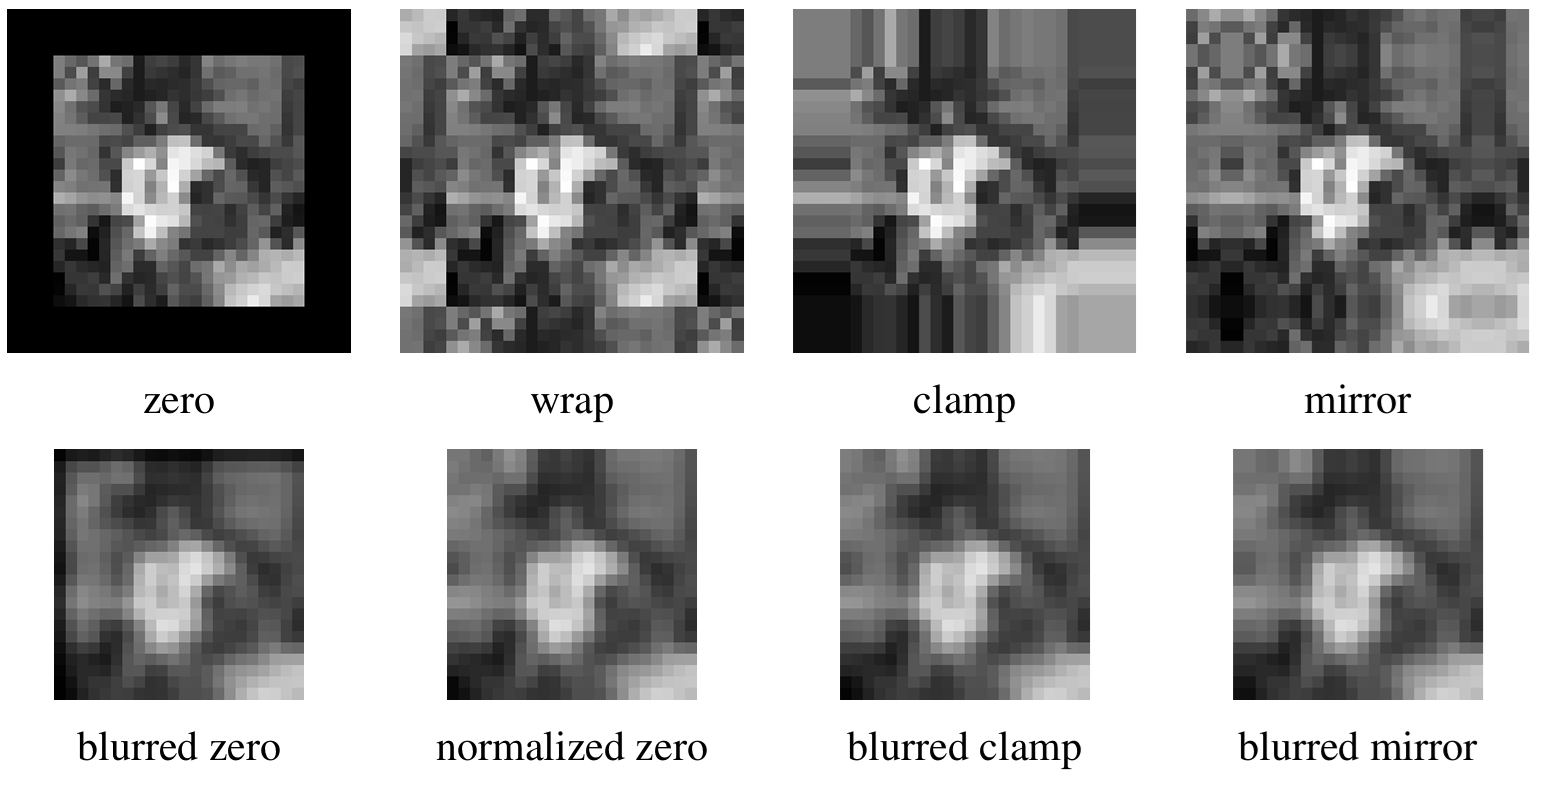
\includegraphics[width=1\textwidth]{images/padding.jpg}
    \caption{Diferite opțiuni de padding}
\end{figure}
\FloatBarrier

Figura arată efectele \textit{padding}-ului unei imagini cu fiecare dintre mecanismele de mai sus și apoi blurarea imaginii rezultate. După cum se poate vedea, \textit{padding}-ul cu zero întunecă marginile, \textit{padding}-ul cu \textit{clamp} (replicare) propagă valorile pixelilor de la margini către interior, \textit{padding}-ul cu \textit{mirror} (reflecție) păstrează culorile aproape de margini. \textit{Padding}-ul cu extindere (nu este prezentat) menține pixelii de la margini fixați (în timpul blur-ului).

O alternativă la \textit{padding} este să încețoșezi imaginea cu canale RGBA zero-\textit{paddate} și apoi să folosești valoarea alpha a imaginii pentru a elimina efectul de întunecare.

\section{Filtre de Binarizare}
În multe situații de prelucrare a imaginilor, este necesar să se ia o decizie finală asupra pixelilor dintr-o imagine sau să se elimine categoric pixelii care se află sub sau peste o anumită valoare, păstrându-i pe ceilalți. Filtrul de binarizare îndeplinește aceste sarcini. Ideea de bază este că se ia un tablou de pixeli, împreună cu un prag, și apoi se aplică o operație fiecărui element al tabloului în funcție de faptul dacă valoarea sa este sub sau peste pragul respectiv. Dacă doriți, puteți considera binarizarea ca o operație de convoluție foarte simplă care utilizează un nucleu de dimensiuni 1 × 1 și apoi efectuează una dintre mai multe operații neliniare pe acel pixel.

\begin{figure}[h!]
    \centering
    \begin{minipage}{0.45\textwidth}
        \centering
        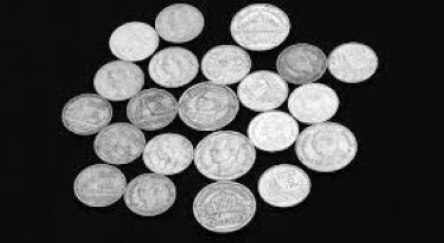
\includegraphics[width=1\textwidth]{images/input_binary_thresholding.jpg}
        \caption{Imagine de Input}
    \end{minipage}
    \hspace{0.01\textwidth}
    \begin{minipage}{0.45\textwidth}
        \centering
        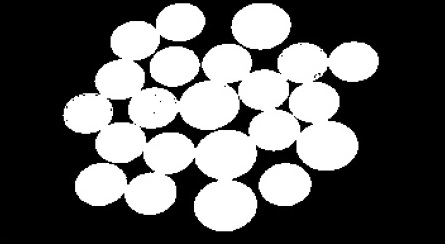
\includegraphics[width=1\textwidth]{images/output_binary_thresholding.jpg}
        \caption{Filtrul Otsu}
    \end{minipage}
\end{figure}
\FloatBarrier

De asemenea, este posibil ca algoritmul de binarizare să determine valoarea optimă a pragului. Aceasta se poate realiza prin utilizarea unui algoritm precum Otsu. Pe scurt, algoritmul lui Otsu ia în considerare toate pragurile posibile și calculează varianța pentru fiecare dintre cele două clase de pixeli (adică clasa de sub prag și clasa de peste prag). Algoritmul lui Otsu minimizează următoarea expresie:
\[
    \sigma_w^2 \equiv w_1(t) \cdot \sigma_1^2 + w_2(t) \cdot \sigma_2^2
\]

unde \( w_1(t) \) și \( w_2(t) \) sunt ponderile relative pentru cele două clase date de numărul de pixeli din fiecare clasă, iar \( \sigma_1^2 \) și \( \sigma_2^2 \) sunt varianțele din fiecare clasă. Se dovedește că minimizarea varianței celor două clase în acest mod este echivalentă cu maximizarea varianței între cele două clase. Deoarece este necesară o căutare exhaustivă a spațiului posibil de praguri, acest proces nu este unul foarte rapid, dar este foarte eficient în determinarea pragului optim pentru separarea pixelilor în două clase distincte.

Filtrul de binarizare prin prag de triunghi este o alta metodă eficientă pentru determinarea automată a pragului optim de binarizare a unei imagini. Această tehnică se bazează pe analiza histogramei imaginii și utilizarea unui algoritm geometric pentru a stabili punctul de prag. Procedura implică mai multe etape:

Prima etapă constă în calcularea histogramei imaginii. Fiecare intensitate este contorizată pentru a obține frecvența de apariție a fiecărei valori de pixel. După obținerea histogramei, se calculează histograma cumulativă. Aceasta ajută la identificarea distribuției totale a intensităților pixelilor și este folosită pentru a trasa linia de referință necesară în algoritmul de binarizare.

Pentru a determina linia de referință, se identifică punctele minim și maxim din histograma cumulativă. Linia de referință este trasată între aceste două puncte și servește ca bază pentru calcularea distanțelor. Pentru fiecare valoare din histograma cumulativă, se calculează distanța față de linia de referință. Această distanță este utilizată pentru a găsi punctul de pe histogramă care se află la cea mai mare distanță față de linia de referință.

Valoarea de intensitate care are cea mai mare distanță față de linia de referință este considerată pragul optim. Acest prag este folosit pentru a binariza imaginea inițială, separând pixelii în două clase: cei cu valori sub prag și cei cu valori peste prag.

Algoritmul de binarizare prin prag de triunghi oferă o metodă robustă și automată pentru binarizarea imaginilor, fiind util în diverse aplicații de prelucrare a imaginilor, unde separarea precisă a obiectelor de fundal este esențială.

\section{Filtre Low-Pass}
Filtrele spațiale de netezire (denumite și de mediere) sunt utilizate pentru a reduce tranzițiile abrupte în intensitate. Deoarece zgomotul aleatoriu constă de obicei din tranziții abrupte în intensitate, o metodă evidentă a netezirii este reducerea zgomotului. Netezirea înainte de resampling-ul imaginii pentru a reduce aliasing-ul este, de asemenea, o practică comună.

\begin{figure}[h!]
    \centering
    \begin{minipage}{0.35\textwidth}
        \centering
        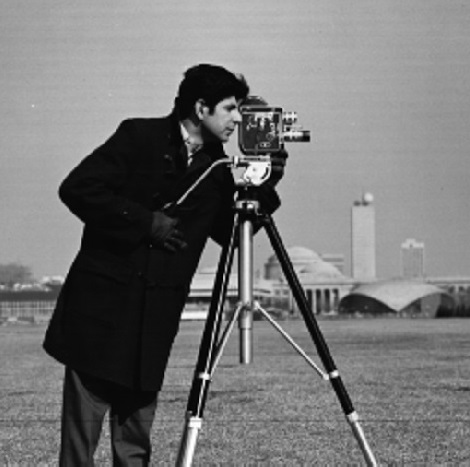
\includegraphics[width=1\textwidth]{images/input_low_pass.jpg}
        \caption{Imagine de Input}
    \end{minipage}
    \hspace{0.01\textwidth}
    \begin{minipage}{0.35\textwidth}
        \centering
        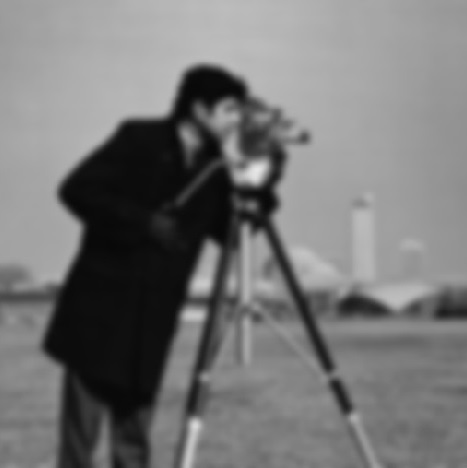
\includegraphics[width=1\textwidth]{images/output_low_pass.jpg}
        \caption{Filtrul Gaussian}
    \end{minipage}
\end{figure}
\FloatBarrier

Netezirea este utilizată pentru a reduce detaliile nerelevante într-o imagine, unde „nerelevant” se referă la regiunile de pixeli care sunt mici în raport cu dimensiunea kernelului filtrului. O altă aplicație este netezirea contururilor false care rezultă din utilizarea unui număr insuficient de niveluri de intensitate într-o imagine. Filtrele de netezire sunt utilizate în combinație cu alte tehnici pentru îmbunătățirea imaginii, cum ar fi tehnicile de procesare a histogramelor și mascare unsharp.

Cel mai simplu filtru low-pass separabil este filtrul de tip cutie, ale cărui coeficienți au aceeași valoare (de obicei 1). Numele „kernel cutie” provine dintr-un kernel de dimensiuni \(m \times n\) cu toți coeficienții egali. Normalizarea kernelului se face prin împărțirea fiecărui coeficient la suma valorilor coeficienților (adică \(1 / mn\) când toți coeficienții sunt 1).

Datorită simplității lor, filtrele de tip cutie sunt potrivite pentru experimentare rapidă și oferă de obicei rezultate de netezire acceptabile vizual. Cu toate acestea, filtrele de tip cutie au limitări care le fac alegeri mai puțin ideale în multe aplicații. Kernelurile Gaussian sunt utilizate frecvent datorită proprietăților lor utile și capacității de a netezi imaginile în mod eficient. Kernelurile Gaussian sunt simetrice circular (isotrope), ceea ce înseamnă că răspunsul lor este independent de orientare.

Kernelul Gaussian este dat de formula:
\[
    w(s,t) = G(s,t) = K e^{-\frac{s^2 + t^2}{2\sigma^2}}
\]

Kernelurile Gaussian sunt singurele kerneluri simetrice circular și separabile, ceea ce le conferă avantaje computaționale similare cu filtrele de tip cutie, dar cu proprietăți suplimentare care le fac ideale pentru procesarea imaginii.

Prin \(r = \sqrt{s^2 + t^2}\), putem scrie ecuația:
\[
    G(r) = K e^{-\frac{r^2}{2\sigma^2}}
\]
unde \(K\) este o constantă de normalizare, iar \(\sigma\) este deviația standard a distribuției Gaussian.

Rezultatul convoluției este deosebit de important în filtrare. De exemplu, filtrarea se poate face în etape succesive, iar același rezultat poate fi obținut printr-o singură etapă de filtrare cu un kernel compozit format ca și convoluție a kernelurilor individuale.

\section{Filtre High-Pass}
Detectarea marginilor este un pas esențial în procesarea imaginilor, deoarece ne permite să identificăm schimbările în intensitate și să găsim contururile obiectelor din imagine. În general, detectarea marginilor implică utilizarea derivatelor de ordinul întâi sau al doilea pentru a determina schimbările în intensitatea pixelilor.

\begin{figure}[h!]
    \centering
    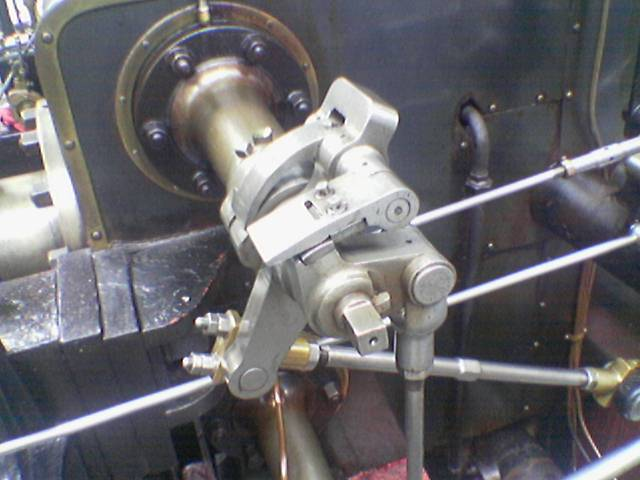
\includegraphics[width=0.4\textwidth]{images/input_edge_detection.jpg}
    \caption{Imagine de Input}
\end{figure}
\FloatBarrier
\begin{figure}[h!]
    \centering
    \begin{minipage}{0.4\textwidth}
        \centering
        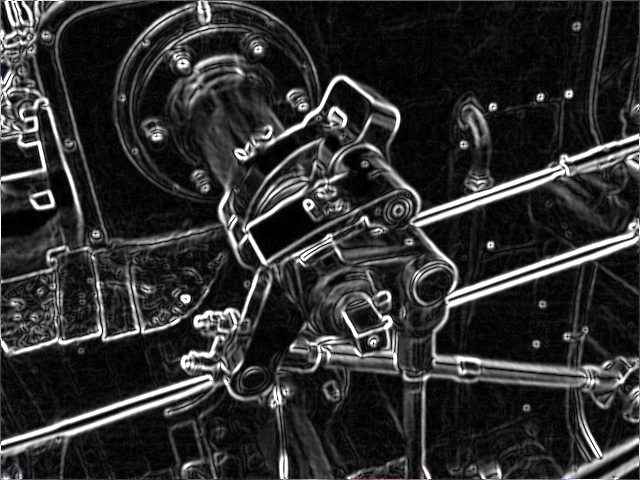
\includegraphics[width=1\textwidth]{images/sobel_edge_detection.jpg}
        \caption{Operatorul Sobel}
    \end{minipage}
    \hspace{0.05\textwidth}
    \begin{minipage}{0.4\textwidth}
        \centering
        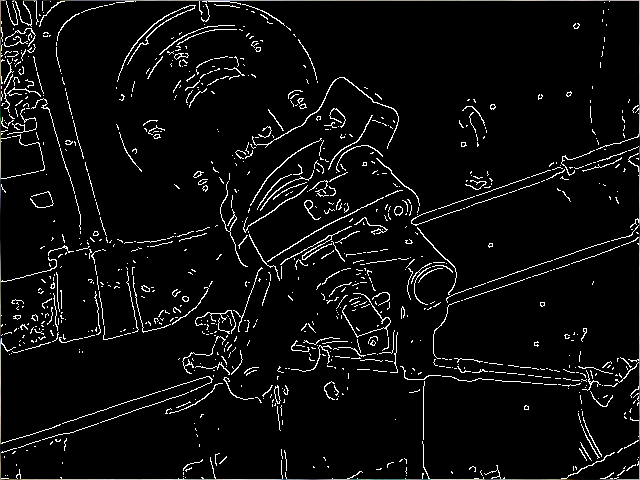
\includegraphics[width=1\textwidth]{images/canny_edge_detection.jpg}
        \caption{Operatorul Canny}
    \end{minipage}
\end{figure}
\FloatBarrier

Instrumentul principal pentru găsirea direcției și intensității marginii într-o imagine este gradientul. Gradientul unei imagini \( f(x, y) \) la un punct arbitrar \((x, y)\) este notat și definit ca vectorul:
\[
    \nabla f(x, y) \equiv \text{grad}[f(x, y)] \equiv \begin{bmatrix} g_x(x, y) \\ g_y(x, y) \end{bmatrix} \equiv \begin{bmatrix} \frac{\partial f(x, y)}{\partial x} \\ \frac{\partial f(x, y)}{\partial y} \end{bmatrix}
\]

Acest vector are proprietatea binecunoscută că indică direcția în care rata de schimbare a \( f \) la \((x, y)\) este maximă.

Magnitudinea \( M(x, y) \) a acestui vector gradient la un punct \((x, y)\) este dată de norma Euclidiană:
\[
    M(x, y) = \| \nabla f(x, y) \| = \sqrt{g_x^2(x, y) + g_y^2(x, y)}
\]

Aceasta este valoarea ratei de schimbare în direcția vectorului gradient la punctul \((x, y)\).

Direcția vectorului gradient la un punct \((x, y)\) este dată de:
\[
    \alpha(x, y) = \tan^{-1} \left( \frac{g_y(x, y)}{g_x(x, y)} \right)
\]

Unghiurile sunt măsurate în sensul acelor de ceasornic față de axa \( x \).

Obținerea gradientului unei imagini necesită calcularea derivatelor parțiale \( \partial f / \partial x \) și \( \partial f / \partial y \) la fiecare locație a pixelilor din imagine. Pentru gradient, utilizăm de obicei o diferență finită înainte sau centrată. Utilizând diferențele înainte, obținem:
\[
    g_x(x, y) = \frac{\partial f(x, y)}{\partial x} \approx f(x+1, y) - f(x, y)
\]
\[
    g_y(x, y) = \frac{\partial f(x, y)}{\partial y} \approx f(x, y+1) - f(x, y)
\]

Kernelurile de mărime 2x2 sunt simple conceptual, dar nu sunt la fel de utile pentru calcularea direcției marginilor precum kernelurile care sunt simetrice în jurul centrelor lor. Cele mai mici astfel de kerneluri au dimensiunea 3x3.

Operatorii Prewitt sunt un alt exemplu de operatori de gradient care utilizează kerneluri de dimensiune 3x3:
\[
    g_x = \frac{\partial f}{\partial x} \approx (z_7 + z_8 + z_9) - (z_1 + z_2 + z_3)
\]
\[
    g_y = \frac{\partial f}{\partial y} \approx (z_3 + z_6 + z_9) - (z_1 + z_4 + z_7)
\]

Acești operatori sunt destul de eficienți în calcularea gradientului, deoarece iau în considerare natura datelor pe părțile opuse ale punctului central și astfel transportă mai multe informații privind direcția unei margini. Operatorii Prewitt, de exemplu, sunt adesea utilizați datorită capacității lor de a oferi o aproximare bună a derivatelor parțiale în imagini.

Un alt set de operatori utilizat frecvent pentru calculul gradientului este setul de operatori Sobel. Acesta folosește, de asemenea, kerneluri de dimensiune 3x3, dar cu un factor suplimentar de ponderare în centrul kernelului, ceea ce ajută la îmbunătățirea sensibilității la zgomot. Kernelurile pentru operatorii Sobel sunt:

\[
    g_x = \frac{\partial f}{\partial x} \approx
    \begin{bmatrix}
        -1 & 0 & 1 \\
        -2 & 0 & 2 \\
        -1 & 0 & 1
    \end{bmatrix}
\]
\[
    g_y = \frac{\partial f}{\partial y} \approx
    \begin{bmatrix}
        -1 & -2 & -1 \\
        0  & 0  & 0  \\
        1  & 2  & 1
    \end{bmatrix}
\]

Utilizând aceste kerneluri, operatorii Sobel calculează gradientul pe direcțiile \( x \) și \( y \), oferind o estimare robustă a direcției și magnitudinii gradientului, ceea ce face ca acești operatori să fie extrem de utili în detectarea marginilor în imagini.

Gradientul morfologici este o altă tehnică în procesarea imaginilor pentru evidențierea marginilor obiectelor. Această tehnică se bazează pe operații morfologice fundamentale precum dilatarea și eroziunea.

Gradientul morfologic este obținut prin calcularea diferenței dintre o imagine dilatată și una erodată. Această operație evidențiază marginile obiectelor din imagine, deoarece dilatarea și eroziunea modifică în mod complementar marginile acestora. Gradientul morfologic \( G \) este definit ca:
\[
    G = (I \oplus B) - (I \ominus B)
\]
unde \( I \) este imaginea binară inițială și \( B \) este elementul structurant utilizat pentru dilatare și eroziune.

\section{Componente conexe}
Identificarea componentelor conexe este o operațiune esențială în procesarea imaginii, utilizată pentru a găsi regiuni de pixeli adiacenți care au aceeași valoare de intensitate. Aceste regiuni sunt denumite componente conexe. Pixelii sunt considerați \textit{N4}-adiacenți dacă sunt adiacenți fie orizontal, fie vertical, și \textit{N8}-adiacenți dacă pot fi și adiacenți diagonal.

Componentele conexe sunt utilizate pe scară largă în diverse aplicații, cum ar fi recunoașterea literelor dintr-un document scanat sau identificarea obiectelor (de exemplu, celule) într-o imagine segmentată și calcularea statisticilor de arie. De-a lungul anilor, au fost dezvoltate o varietate de algoritmi eficienți pentru a găsi astfel de componente. Astfel de algoritmi sunt de obicei incluși în bibliotecile de procesare a imaginii.

După ce o imagine binară sau multivalorată a fost segmentată în componentele sale conexe, este util să calculăm statisticile de arie pentru fiecare regiune individuală $\mathcal{R}$. Astfel de statistici includ:
\begin{itemize}
    \item \textbf{Aria} (numărul de pixeli);
    \item \textbf{Perimetrul} (numărul de pixeli de la margine);
    \item \textbf{Centroidul} (valorile medii $x$ și $y$);
    \item \textbf{Momentul de ordinul doi},
          \[
              M = \sum_{(x,y) \in \mathcal{R}} \begin{bmatrix}
                  x - \bar{x} \\
                  y - \bar{y}
              \end{bmatrix}
              \begin{bmatrix}
                  x - \bar{x} & y - \bar{y}
              \end{bmatrix},
          \]
          de la care se pot calcula orientarea și lungimile axelor major și minor folosind analiza valorilor proprii.
\end{itemize}

Aceste statistici pot fi apoi utilizate pentru prelucrarea ulterioară, de exemplu, pentru sortarea regiunilor în funcție de dimensiune (pentru a considera mai întâi regiunile cele mai mari) sau pentru potrivirea preliminară a regiunilor din imagini diferite.

Boxurile de delimitare sunt utilizate pentru a încadra componentele conexe identificate într-o imagine. Fiecare componentă conexă este înconjurată de un dreptunghi minim care cuprinde toți pixelii din componenta respectivă. Parametrii acestui dreptunghi sunt:
\begin{itemize}
    \item \textbf{Coordonatele colțului din stânga-sus} $(x_{min}, y_{min})$;
    \item \textbf{Lățimea și înălțimea} $(w, h)$.
\end{itemize}

Aceste boxuri de delimitare sunt esențiale în diverse aplicații de vizualizare și analiză a imaginii, oferind un mijloc simplu și eficient de localizare și izolare a componentelor de interes.

Componentelor conexe și utilizarea boxurilor de delimitare sunt instrumente fundamentale în procesarea imaginilor, permițând izolarea eficientă și analiza precisă a regiunilor de interes în imagini binare și multivalorate.

\section{Contururi}
Algoritmii precum detectorul de margini Canny pot fi utilizați pentru a găsi pixeli de margine care separă diferite segmente într-o imagine, dar nu ne oferă informații despre acele margini ca entități în sine. Pasul următor este să asamblăm acei pixeli de margine în contururi. Un contur este o listă de puncte care reprezintă, într-un fel sau altul, o curbă într-o imagine. Această reprezentare poate varia în funcție de circumstanțele specifice.

Există multe modalități de a reprezenta o curbă. Contururile pot fi reprezentate prin secvențe de puncte 2D. De exemplu, o astfel de reprezentare este lanțul Freeman, în care fiecare punct este reprezentat ca un „pas” într-o direcție dată de la punctul anterior. Deși secvențele de puncte 2D sunt cele mai comune, există și alte modalități de a reprezenta contururile.

Funcțiile de calcul al contururilor pornesc de la imagini binare. Acestea pot folosi imagini create de algoritmi de detectare a marginilor, cum ar fi detectorul Canny, sau imagini create prin aplicarea unor funcții de prag, în care marginile sunt implicite ca limite între regiuni pozitive și negative.

Înainte de a detalia modul de extragere a contururilor, este important să înțelegem ce este un contur și cum pot fi relaționate grupurile de contururi între ele. Un concept deosebit de important este arborele de contururi, care encodează relațiile de includere între contururi.

Un arbore de contururi este o structură ierarhică în care fiecare nod reprezintă un contur. Fiecare nod poate avea copii care sunt contururi incluse în conturul părinte. Această structură ierarhică poate fi reprezentată prin array-uri în care fiecare intrare reprezintă un contur specific. Fiecare intrare conține un set de patru întregi care indică alte noduri în ierarhie cu o relație particulară față de nodul curent. Dacă o relație specifică nu există, elementul corespunzător din structură este setat la -1 (de exemplu, ID-ul părintelui pentru nodul rădăcină ar avea valoarea -1 deoarece nu are părinte).

\begin{figure}[h!]
    \centering
    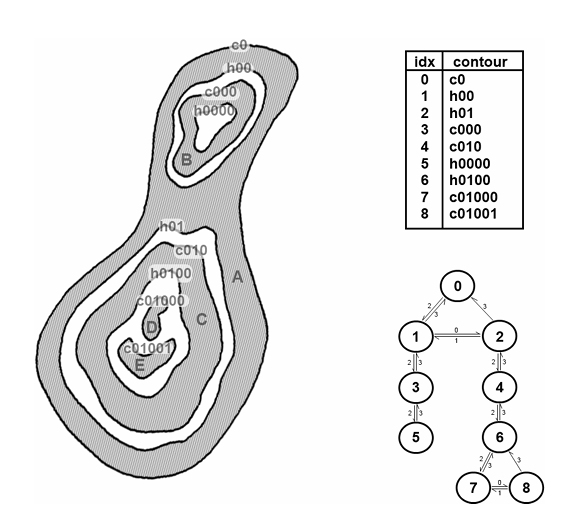
\includegraphics[width=0.75\textwidth]{images/contours.jpg}
    \caption{Regiuni}
\end{figure}
\FloatBarrier

Imaginea de mai sus conține mai multe regiuni pe un fundal alb. Contururile acestor regiuni pot fi găsite și aranjate într-un arbore de contururi. De exemplu, dacă avem cinci regiuni, rezultând un total de nouă contururi (incluzând atât marginile exterioare, cât și cele interioare ale fiecărei regiuni), fiecare nod din arbore va avea ca și copii acele contururi care sunt incluse în conturul respectiv. Arborele rezultat poate fi vizualizat, arătând legăturile valide și relațiile dintre noduri.

Contururile sunt structuri esențiale în procesarea imaginii, reprezentând margini și forme într-o manieră organizată. Înțelegerea și utilizarea contururilor permite realizarea unor operațiuni avansate de analiză și manipulare a imaginii, inclusiv identificarea obiectelor și segmentarea precisă a regiunilor de interes.

\section{Analiza componentelor conexe}
După segmentarea unei imagini, de obicei prin binarizare, putem folosi analiza componentelor conexe pentru a izola și procesa eficient regiunile rezultate ale imaginii una câte una. Analiza componentelor conexe are ca scop etichetarea regiunilor conectate dintr-o imagine binară. Prin etichetarea acestor regiuni, putem izola și analiza fiecare componentă în parte.

\begin{enumerate}
    \item \textbf{Intrare}: Intrarea este o imagine binară în care prim-planul și fundalul sunt clar definite.
    \item \textbf{Etichetarea}: Fiecare pixel din prim-plan primește o etichetă, indicând care componentă conexă o reprezintă. Acest lucru are ca rezultat o hartă de pixeli etichetați unde toți pixelii din aceeași componentă conexă împărtășesc aceeași etichetă.
    \item \textbf{Ieșire}: Ieșirea este o imagine etichetată și, opțional, un set de statistici pentru fiecare componentă conexă, cum ar fi aria, dreptunghiul de delimitare și centrul de masă.
\end{enumerate}
Analiza componentelor conexe este destul de populară în algoritmii de segmentare a fundalului ca filtru post-procesare care elimină petele mici de zgomot și în probleme cum ar fi OCR, unde există un prim-plan bine definit de extras. Este esențial ca această operație de bază să fie rapidă.

\section{Operații logice}
Operațiile logice lucrează cu variabile și expresii TRUE (de obicei denotate prin 1) și FALSE (de obicei denotate prin 0). În cazul nostru, aceasta înseamnă imagini binare compuse din pixeli de prim-plan (valorați cu 1) și un fundal format din pixeli cu valoarea 0.

Utilizăm operatori logici și de set pe imagini binare folosind două abordări principale:
\begin{enumerate}
    \item Utilizăm coordonatele regiunilor individuale de pixeli de prim-plan într-o singură imagine ca seturi.
    \item Lucrăm cu una sau mai multe imagini de aceeași dimensiune și efectuăm operații logice între pixelii corespunzători din aceste matrice.
\end{enumerate}

În prima categorie, o imagine binară poate fi privită ca o diagramă Venn în care coordonatele regiunilor de pixeli valorați cu 1 sunt tratate ca seturi. Uniunea acestor seturi cu setul compus din pixeli valorați cu 0 formează universul setului, Æ. De exemplu, pentru o imagine binară cu două regiuni de pixeli valorați cu 1, $R_1$ și $R_2$, putem determina dacă regiunile se suprapun (au cel puțin o pereche de coordonate comune) prin efectuarea operației de intersecție a seturilor $R_1 \cap R_2$.

În a doua abordare, efectuăm operații logice pe pixelii unei imagini binare sau pe pixelii corespunzători din două sau mai multe imagini binare de aceeași dimensiune. Operatorii logici pot fi definiți în termeni de tabele de adevăr. Operația logică AND (denotată și $\wedge$) produce 1 (TRUE) doar când ambii $a$ și $b$ sunt 1. În mod similar, OR ($\vee$) produce 1 când $a$ sau $b$ sau ambii sunt 1, iar operatorul NOT ($\neg$) este auto-explicativ. Operatorii AND și OR sunt \textit{elementwise} în acest context, operând pe perechi de pixeli corespunzători între imagini.

\begin{figure}[h!]
    \centering
    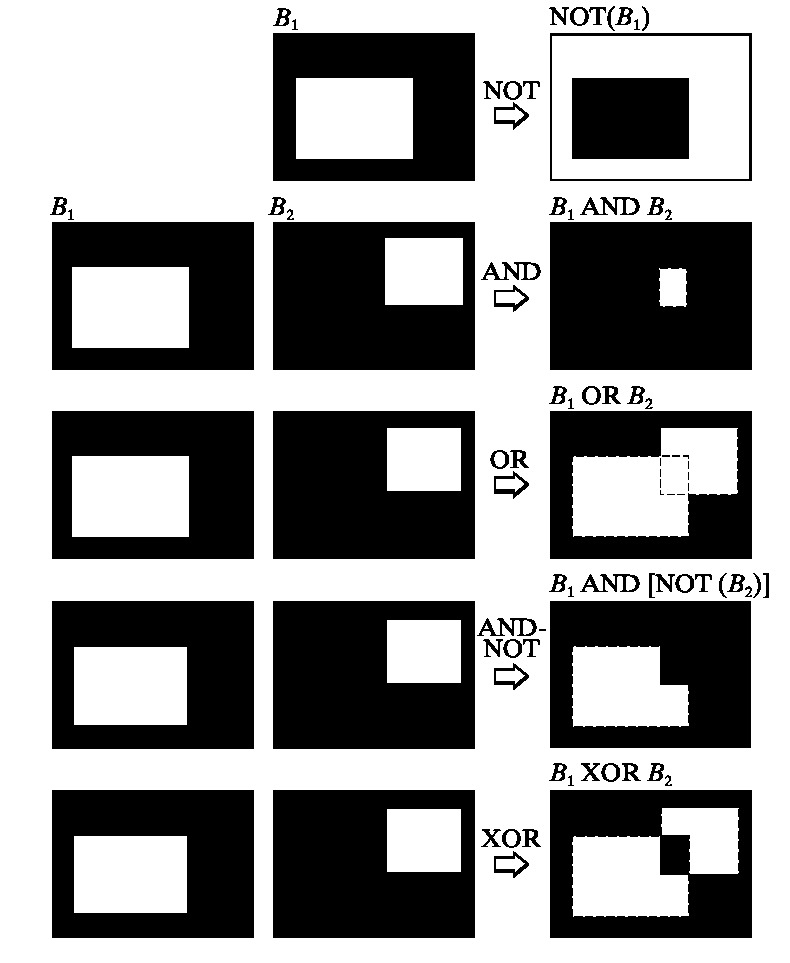
\includegraphics[width=0.6\textwidth]{images/logical_operations.jpg}
    \caption{Operații logice}
\end{figure}
\FloatBarrier

Figura ilustrează operații logice folosind a doua abordare discutată. NOT al imaginii binare B1 este o matrice obținută prin schimbarea tuturor pixelilor valorați cu 1 în 0 și invers. AND dintre B1 și B2 conține 1 în toate locațiile unde elementele corespunzătoare ale B1 și B2 sunt 1; operația produce 0 în altă parte. OR dintre cele două imagini este o matrice care conține 1 în locațiile unde elementele corespunzătoare ale B1 sau B2 sau ambele sunt 1. XOR (exclusive OR) produce 1 în locațiile unde elementele corespunzătoare ale B1 sau B2 (dar nu ambele) sunt 1.

Putem obține aceleași rezultate folosind prima abordare discutată mai sus. Începem prin etichetarea regiunilor individuale valorați cu 1 în fiecare dintre cele două imagini. Să notăm cu A și B seturile de coordonate ale tuturor pixelilor valorați cu 1 în imaginile B1 și B2. Apoi formăm o singură matrice prin aplicarea operației OR între cele două imagini, păstrând etichetele A și B. Rezultatul ar arăta ca matricea $B_1 \vee B_2$, dar cu cele două regiuni albe etichetate A și B, asemănătoare unui diagramă Venn.

\section{Operații morfologice}
Morfologia imaginii este un subiect de sine stătător ce cuprinde un număr mare de operații morfologice care au fost dezvoltate în special în primii ani ai viziunii computerizate. Majoritatea operațiilor au fost dezvoltate pentru un scop specific sau altul, iar unele dintre acestea și-au găsit o utilitate mai largă de-a lungul anilor. Practic, toate operațiile morfologice se bazează pe doar două operații primitive.

Transformările morfologice de bază se numesc dilatare și eroziune și apar într-o varietate de contexte, cum ar fi eliminarea zgomotului, izolarea elementelor individuale și unirea elementelor disparate într-o imagine. Operațiile morfologice mai sofisticate, bazate pe aceste două operații de bază, pot fi utilizate pentru a găsi vârfuri de intensitate (sau găuri) într-o imagine și pentru a defini (încă o dată) o formă particulară a gradientului de imagine.

\begin{figure}[h!]
    \centering
    \begin{minipage}{0.25\textwidth}
        \centering
        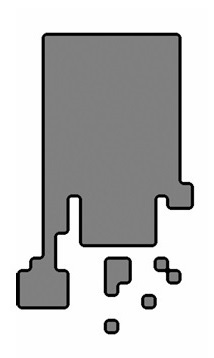
\includegraphics[width=1\textwidth]{images/input_dilate.jpg}
        \caption{Imagine de Input}
    \end{minipage}
    \hspace{0.05\textwidth}
    \begin{minipage}{0.25\textwidth}
        \centering
        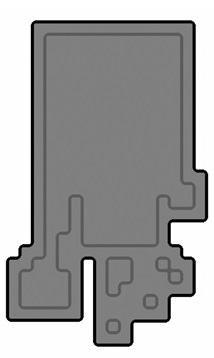
\includegraphics[width=1\textwidth]{images/output_dilate.jpg}
        \caption{Operația de dilatare}
    \end{minipage}
\end{figure}
\FloatBarrier

Dilatarea este o convoluție a unei imagini cu un nucleu în care orice pixel dat este înlocuit cu maximul local al tuturor valorilor pixelilor acoperiți de nucleu. Așa cum am menționat anterior, aceasta este un exemplu de operație neliniară, deci nucleul nu poate fi exprimat în forma arătată. Cel mai adesea, nucleul folosit pentru dilatare este un nucleu pătrat „solid” sau uneori un disc, cu punctul de ancorare în centru. Efectul dilatării este de a face ca regiunile umplute dintr-o imagine să crească.

\begin{figure}[h!]
    \centering
    \begin{minipage}{0.25\textwidth}
        \centering
        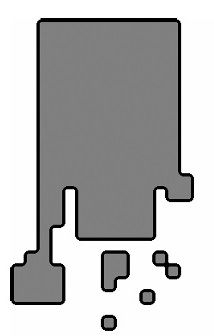
\includegraphics[width=1\textwidth]{images/input_erode.jpg}
        \caption{Imagine de Input}
    \end{minipage}
    \hspace{0.05\textwidth}
    \begin{minipage}{0.25\textwidth}
        \centering
        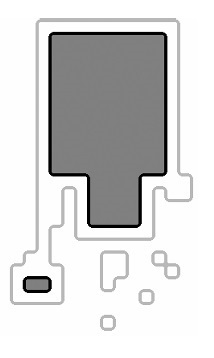
\includegraphics[width=1\textwidth]{images/output_erode.jpg}
        \caption{Operația de erodare}
    \end{minipage}
\end{figure}
\FloatBarrier

Eroziunea este operația opusă. Acțiunea operatorului de eroziune este echivalentă cu calcularea unui minim local peste zona nucleului. În general, în timp ce dilatarea extinde o regiune luminoasă, eroziunea reduce o astfel de regiune luminoasă. Mai mult, dilatarea va tinde să umple concavitățile, iar eroziunea va tinde să elimine proeminențele. Desigur, rezultatul exact va depinde de nucleu, dar aceste afirmații sunt în general adevărate atâta timp cât nucleul este convex și umplut.

\begin{figure}[h!]
    \centering
    \begin{minipage}{0.25\textwidth}
        \centering
        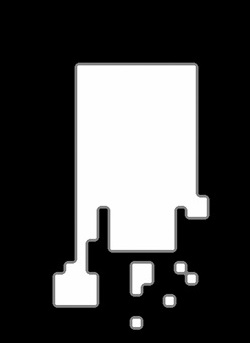
\includegraphics[width=1\textwidth]{images/input_open.jpg}
        \caption{Imagine de Input}
    \end{minipage}
    \hspace{0.05\textwidth}
    \begin{minipage}{0.25\textwidth}
        \centering
        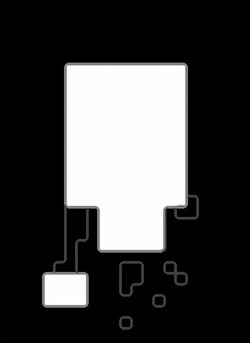
\includegraphics[width=1\textwidth]{images/output_open.jpg}
        \caption{Operația de deschidere}
    \end{minipage}
\end{figure}
\FloatBarrier

Operațiile de deschiderea și închiderea, sunt de fapt combinații simple ale operatorilor de eroziune și dilatare. În cazul deschiderii, erodăm mai întâi și apoi dilatăm. Deschiderea este adesea folosită pentru a număra regiunile într-o imagine binară. De exemplu, dacă am pragat o imagine a celulelor pe o lamă de microscop, am putea folosi deschiderea pentru a separa celulele care sunt aproape una de cealaltă înainte de a număra regiunile.

\begin{figure}[h!]
    \centering
    \begin{minipage}{0.25\textwidth}
        \centering
        
\includegraphics[width=1\textwidth]{images/input_close.jpg}
        \caption{Imagine de Input}
    \end{minipage}
    \hspace{0.05\textwidth}
    \begin{minipage}{0.25\textwidth}
        \centering
        
\includegraphics[width=1\textwidth]{images/output_close.jpg}
        \caption{Operația de închidere}
    \end{minipage}
\end{figure}
\FloatBarrier

În cazul închiderii, dilatăm mai întâi și apoi erodăm. Închiderea este utilizată în majoritatea algoritmilor de componente conexe mai sofisticați pentru a reduce segmentele nedorite sau generate de zgomot. Pentru componentele conexe, de obicei se efectuează mai întâi o eroziune sau o operație de închidere pentru a elimina elementele care apar doar din zgomot, și apoi se folosește o operație de deschidere pentru a conecta regiunile mari din apropiere. Observați că, deși rezultatul final al utilizării deschiderii sau închiderii este similar cu utilizarea eroziunii sau dilatării, aceste noi operații tind să păstreze mai precis aria regiunilor conexe.

\section{Transformări geometrice}
Utilizăm transformările geometrice pentru a modifica aranjamentul spațial al pixelilor dintr-o imagine. Transformările geometrice ale imaginilor digitale constau în două operații de bază:
\begin{enumerate}
    \item Transformarea spațială a coordonatelor.
    \item Interpolarea intensității care atribuie valori de intensitate pixelilor transformați spațial.
\end{enumerate}

Transformarea coordonatelor poate fi exprimată astfel:
\[
    \begin{bmatrix}
        x' \\
        y'
    \end{bmatrix}
    =
    T
    \begin{bmatrix}
        x \\
        y
    \end{bmatrix}
    =
    \begin{bmatrix}
        t_{11} & t_{12} \\
        t_{21} & t_{22}
    \end{bmatrix}
    \begin{bmatrix}
        x \\
        y
    \end{bmatrix}
\]
unde $(x, y)$ sunt coordonatele pixelilor în imaginea originală și $(x', y')$ sunt coordonatele pixelilor corespunzători din imaginea transformată. De exemplu, transformarea $(x', y') = (x/2, y/2)$ micșorează imaginea originală la jumătate în ambele direcții spațiale.

Ne interesează așa-numitele \textit{transformări afine}, care includ scalarea, translația, rotația și deformarea. Caracteristica principală a unei transformări afine în 2D este că păstrează punctele, liniile drepte și planele. Ecuația definită anterior poate fi folosită pentru a exprima transformările menționate mai sus, cu excepția translației, care ar necesita adăugarea unui vector constant 2D în partea dreaptă a ecuației. Cu toate acestea, este posibil să folosim coordonate omogene pentru a exprima toate cele patru transformări afine folosind o singură matrice 3x3 în următoarea formă generală:
\[
    \begin{bmatrix}
        x' \\
        y' \\
        1
    \end{bmatrix}
    =
    \begin{bmatrix}
        a_{11} & a_{12} & a_{13} \\
        a_{21} & a_{22} & a_{23} \\
        0      & 0      & 1
    \end{bmatrix}
    \begin{bmatrix}
        x \\
        y \\
        1
    \end{bmatrix}
\]

Această transformare poate scala, roti, translata sau deforma o imagine, în funcție de valorile alese pentru elementele matricei A.

Transformarea anterioară mută coordonatele pixelilor dintr-o imagine în locații noi. Pentru a finaliza procesul, trebuie să atribuim valori de intensitate pixelilor relocați. Această sarcină este realizată folosind \textit{interpolarea intensității}.

Putem utiliza ecuația în două moduri de bază. Primul este \textit{cartografierea directă}, care constă în scanarea pixelilor imaginii de intrare și, la fiecare locație $(x, y)$, calcularea locației spațiale $(x', y')$ a pixelului corespunzător în imaginea de ieșire folosind direct ecuația.

Al doilea mod, numit \textit{cartografiere inversă}, scanează locațiile pixelilor de ieșire și, la fiecare locație $(x', y')$, calculează locația corespunzătoare în imaginea de intrare folosind $(x, y) = A^{-1}(x', y')$. Apoi interpolează printre cei mai apropiați pixeli de intrare pentru a determina intensitatea valorii pixelului de ieșire.

\section{Transformata Hough}
Adesea, trebuie să lucrăm în medii neorganizate în care avem doar o hartă de margini și nicio informație despre unde ar putea fi obiectele de interes. În astfel de situații, toți pixelii sunt candidați pentru legături și, astfel, trebuie să fie acceptați sau eliminați pe baza unor proprietăți globale definite. În această secțiune, dezvoltăm o abordare bazată pe faptul dacă seturile de pixeli se află pe curbe de o anumită formă. Odată detectate, aceste curbe formează marginile sau contururile regiunilor de interes.

Dat fiind $n$ puncte într-o imagine, presupunem că dorim să găsim submulțimi ale acestor puncte care se află pe linii drepte. O soluție posibilă este să găsim toate liniile determinate de fiecare pereche de puncte, apoi să găsim toate submulțimile de puncte care sunt aproape de liniile particulare. Această abordare implică găsirea $\frac{n(n-1)}{2} \sim n^2$ linii, apoi efectuarea $n \left(\frac{n(n-1)}{2}\right) \sim n^3$ comparații ale fiecărui punct pentru toate liniile.

Transformata Hough, propusă de Hough în 1962, este o metodă alternativă pentru detectarea liniilor. Fie $(x_i, y_i)$ un punct în planul $xy$ și considerăm ecuația generală a unei linii în formă de panta-interceptare: $y_i = ax_i + b$. Infinit de multe linii trec prin $(x_i, y_i)$, dar toate satisfac ecuația $y_i = ax_i + b$ pentru valori variate ale lui $a$ și $b$. Totuși, scriind această ecuație ca $b = -x_i a + y_i$ și considerând planul $ab$ (numit și spațiul parametrilor), obținem ecuația unei singure linii pentru un punct fix $(x_i, y_i)$.
\[
    x \cos \theta + y \sin \theta = \rho
\]

\begin{figure}[h!]
    \centering
    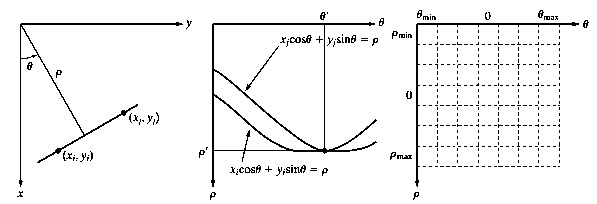
\includegraphics[width=1\textwidth]{images/hough_space.jpg}
    \caption{Interpretare geometrică}
\end{figure}
\FloatBarrier

Figura ilustrează interpretarea geometrică a parametrilor $\rho$ și $\theta$. O linie orizontală are $\theta = 0^\circ$, cu $\rho$ egal cu interceptul pozitiv pe axa $x$. Similar, o linie verticală are $\theta = 90^\circ$, cu $\rho$ egal cu interceptul pozitiv pe axa $y$, sau $\theta = -90^\circ$, cu $\rho$ egal cu interceptul negativ pe axa $y$.

Atracția computațională a transformatei Hough provine din subdivizarea spațiului parametrilor $\rho, \theta$ în celule de acumulare. Procedura constă în incrementarea $\theta$ și calcularea valorilor corespunzătoare $\rho$ folosind ecuația:
\[
    \rho = x_i \cos \theta + y_i \sin \theta
\]

Celula la coordonatele $(i, j)$ cu valoare de acumulare $A(i, j)$ corespunde pătratului asociat cu coordonatele spațiului parametrilor $(\rho, \theta)$. Inițial, aceste celule sunt setate la zero. Apoi, pentru fiecare punct non-fundal $(x_k, y_k)$ în planul $xy$, incrementăm $\theta$ și calculăm $\rho$ folosind ecuația de mai sus. Valorile rezultate $\rho$ sunt rotunjite la cea mai apropiată valoare permisă de-a lungul axei $\rho$ și se actualizează celula de acumulare $A(p, q)$.

Transformata Hough este un instrument puternic pentru detectarea formelor într-o imagine și este folosită în multe aplicații practice, de la analiza imaginilor medicale la navigația autonomă.

\begin{figure}[h!]
    \centering
    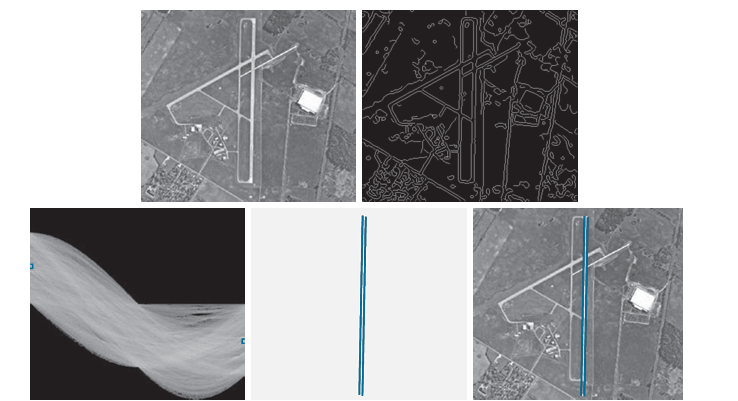
\includegraphics[width=1\textwidth]{images/airport.jpg}
    \caption{Detectarea liniilor unei piste de aterizare}
\end{figure}
\FloatBarrier

Figura de mai sus arată o imagine aeriană a unui aeroport. Obiectivul acestui exemplu este să utilizăm transformata Hough pentru a extrage cele două margini care definesc pista principală. O soluție la o astfel de problemă ar putea fi de interes, de exemplu, în aplicații care implică navigația aeriană autonomă.

Primul pas este obținerea unei hărți de margini. Figura a doua arată harta de margini obținută folosind algoritmul Canny. În scopul calculării transformatei Hough, rezultate similare pot fi obținute utilizând oricare dintre celelalte tehnici de detecție a marginilor existente. Figura a treia arată spațiul parametrilor Hough obținut folosind incrementări de 1° pentru $\theta$ și incrementări de un pixel pentru $\rho$.

Pista de interes este orientată aproximativ 1° față de direcția nord, astfel încât selectăm celulele corespunzătoare la ±90° și care conțin numărul cel mai mare, deoarece pistele sunt cele mai lungi linii orientate în aceste direcții. Cutiile mici de pe marginile imaginii trei evidențiază aceste celule. După cum s-a menționat anterior în legătură cu figura a doua, transformata Hough arată adiacență la marginile imaginii. O altă modalitate de interpretare a acestei proprietăți este că o linie orientată la +90° și o linie orientată la −90° sunt echivalente (adică, ambele sunt verticale). Imaginea a patra arată liniile corespunzătoare celor două celule de acumulare discutate anterior, iar figura a cincea arată liniile suprapuse pe imaginea originală. Liniile au fost obținute prin unirea tuturor spațiilor care nu depășesc 20\% (aproximativ 100 pixeli) din înălțimea imaginii. Aceste linii corespund clar marginilor pistei de interes.

Observați că singura informație necesară pentru a rezolva această problemă a fost orientarea pistei și poziția observatorului în raport cu aceasta. Cu alte cuvinte, un vehicul care navighează autonom ar ști că, dacă pista de interes este orientată spre nord, iar direcția de deplasare a vehiculului este, de asemenea, spre nord, pista ar trebui să apară vertical în imagine. Alte orientări relative sunt tratate într-un mod similar. Orientările pistelor din întreaga lume sunt disponibile în hărțile de zbor, iar direcția de deplasare poate fi obținută cu ușurință folosind informațiile de la GPS (Global Positioning System). Aceste informații ar putea fi folosite, de asemenea, pentru a calcula distanța dintre vehicul și pistă, permițând astfel estimarea unor parametri, cum ar fi lungimea așteptată a liniilor în raport cu dimensiunea imaginii.

\section{Distanța de la un punct la o dreaptă}
Considerăm o dreaptă în planul $xy$ definită de două puncte $(x_1, y_1)$ și $(x_2, y_2)$. Ecuația generală a acestei drepte poate fi scrisă în forma:
\[
    ax + by + c = 0
\]
unde:
\begin{itemize}
    \item coeficientul $a$ este diferența dintre ordonatele celor două puncte ale dreptei:
          \[
              a = y_1 - y_2
          \]
    \item coeficientul $b$ este diferența dintre abscisele celor două puncte ale dreptei:
          \[
              b = x_2 - x_1
          \]
    \item termenul liber $c$ este dat de formula:
          \[
              c = x_1 y_2 - x_2 y_1
          \]
\end{itemize}

De asemenea, considerăm un punct $(x_0, y_0)$ în planul $xy$. Distanța de la acest punct la dreaptă este dată de formula:
\[
    d = \frac{|a x_0 + b y_0 + c|}{\sqrt{a^2 + b^2}}
\]

Această formulă ne permite să calculăm distanța perpendiculară de la un punct dat la o dreaptă specificată prin două puncte în planul $xy$.

\section{Punctul de intersecție a două drepte}
Considerăm două drepte în planul $xy$, fiecare definită de două puncte. Prima dreaptă este definită de punctele $(x_1, y_1)$ și $(x_2, y_2)$, iar a doua dreaptă este definită de punctele $(x_3, y_3)$ și $(x_4, y_4)$.

Ecuația generală a unei drepte în planul $xy$ poate fi scrisă în forma:
\[
    Ax + By = C
\]

Pentru prima dreaptă, ecuația este:
\[
    A_1 x + B_1 y = C_1
\]
unde:
\[
    A_1 = y_2 - y_1, \quad B_1 = x_1 - x_2, \quad C_1 = A_1 x_1 + B_1 y_1
\]

Pentru a doua dreaptă, ecuația este:
\[
    A_2 x + B_2 y = C_2
\]
unde:
\[
    A_2 = y_4 - y_3, \quad B_2 = x_3 - x_4, \quad C_2 = A_2 x_3 + B_2 y_3
\]

Punctul de intersecție $(x, y)$ al celor două drepte poate fi determinat rezolvând sistemul de ecuații liniare:
\[
    \begin{cases}
        A_1 x + B_1 y = C_1 \\
        A_2 x + B_2 y = C_2
    \end{cases}
\]

Pentru a rezolva acest sistem, folosim determinantul:
\[
    D = A_1 B_2 - A_2 B_1
\]

Dacă $D \neq 0$, sistemul are o soluție unică, iar coordonatele punctului de intersecție sunt date de:
\[
    x = \frac{B_2 C_1 - B_1 C_2}{D}
\]
\[
    y = \frac{A_1 C_2 - A_2 C_1}{D}
\]

Dacă $D = 0$, dreptele sunt paralele și nu se intersectează într-un punct finit.

\section{Distanța dintre două drepte}
Considerăm două drepte în planul $xy$. Prima dreaptă este definită de coordonatele $(x_1, y_1)$ și $(x_2, y_2)$, iar a doua dreaptă de referință este definită de coordonatele $(x_r, y_r)$ și $(x_s, y_s)$.

Pentru a determina poziția relativă a unei drepte față de dreapta de referință, mai întâi calculăm punctul mediu al primei drepte. Coordonatele punctului mediu $(x_m, y_m)$ sunt date de:

\[
    x_m = \frac{x_1 + x_2}{2}
\]
\[
    y_m = \frac{y_1 + y_2}{2}
\]

Distanța dintre punctul mediu $(x_m, y_m)$ și dreapta de referință este calculată folosind formula:
\[
    d = (x_m - x_r) \cdot (y_s - y_r) - (y_m - y_r) \cdot (x_s - x_r)
\]

Această formulă este derivată din proprietățile determinantului și reprezintă o măsură a distanței semnate dintre punctul mediu și dreapta de referință. Semnul distanței indică poziția relativă a punctului mediu față de dreapta de referință. Astfel:
\begin{itemize}
    \item dacă $d > 0$, punctul mediu $(x_m, y_m)$ se află de o parte a dreptei de referință,
    \item  dacă $d < 0$, punctul mediu $(x_m, y_m)$ se află de cealaltă parte a dreptei de referință,
    \item  dacă $d = 0$, punctul mediu $(x_m, y_m)$ se află exact pe dreapta de referință.
\end{itemize}

\section{Determinarea unei drepte care trece printr-un punct}
Considerăm un punct dat $(x_0, y_0)$ în planul $xy$ și o pantă $m$. Obiectivul este de a determina ecuația dreptei care trece prin acest punct și are panta specificată.

Ecuația generală a unei drepte în planul $xy$ este dată de:
\[
    y = mx + b
\]
unde $m$ este panta dreptei și $b$ este interceptul pe axa $y$.

Pentru a determina interceptul $b$, utilizăm coordonatele punctului $(x_0, y_0)$. Substituim aceste coordonate în ecuația generală a dreptei:
\[
    y_0 = mx_0 + b
\]

Rezolvăm pentru $b$:
\[
    b = y_0 - mx_0
\]

Pentru a determina punctele de start și de sfârșit ale dreptei în cadrul unui sistem de coordonate de dimensiune $(W, H)$, procedăm în funcție de direcția în care dorim să extindem dreapta.
\begin{enumerate}
    \item Extinderea dreptei pe direcția orizontală
          \begin{itemize}
              \item Punctul de start $(x_s, y_s)$:
                    \[
                        x_s = 0, \quad y_s = b
                    \]
              \item Punctul de sfârșit $(x_e, y_e)$:
                    \[
                        x_e = W, \quad y_e = mW + b
                    \]
          \end{itemize}
    \item Extinderea dreptei pe direcția verticală
          \begin{itemize}
              \item  Dacă $m \neq 0$:
                    \begin{itemize}

                        \item Punctul de start $(x_s, y_s)$:
                              \[
                                  x_s = -\frac{b}{m}, \quad y_s = 0
                              \]
                        \item Punctul de sfârșit $(x_e, y_e)$:
                              \[
                                  x_e = \frac{H - b}{m}, \quad y_e = H
                              \]
                    \end{itemize}
              \item Dacă $m = 0$:
                    \begin{itemize}
                        \item Punctul de start $(x_s, y_s)$ și punctul de sfârșit $(x_e, y_e)$:
                              \[
                                  x_s = x_e = x_0, \quad y_s = 0, \quad y_e = H
                              \]
                    \end{itemize}

          \end{itemize}
\end{enumerate}

Astfel, ecuația dreptei și punctele de start și sfârșit pot fi determinate folosind panta $m$ și punctul dat $(x_0, y_0)$. Acest proces ne permite să trasăm o dreaptă definită clar în cadrul unui sistem de coordonate specificat.

\chapter{Prezentarea aplicației}
\section{Arhitectura}
Vom începe prin a detalia arhitectura modulară a aplicației, accentuând modul în care fiecare componentă specifică aduce un aport semnificativ la funcționalitatea de ansamblu. Această arhitectură este concepută pentru a sprijini extensibilitatea, ușurința în mentenanță și posibilitatea de a testa independent fiecare modul, facilitând astfel adaptarea și scalarea aplicației în funcție de necesități.

Intrarea în aplicație este gestionată de proiectul Application, care cuprinde funcția main. Aceasta are rolul de a inițializa și lansa interfața grafice, fiind punctul de interacțiune primar pentru utilizatori. Structura simplificată a funcției main este proiectată pentru a oferi un punct de start clar și eficient, minimizând dependențele inițiale și asigurând o încărcare rapidă și neîntreruptă a aplicației.

Interfața de utilizator a aplicației este orchestrată prin intermediul proiectului UserInterface, care este subordonat proiectului principal Application. Acest modul este esențial pentru gestionarea interacțiunii cu utilizatorul și include toate elementele de GUI necesare pentru o navigare intuitivă și eficientă în cadrul aplicației.

Proiectul UserInterface cuprinde, în principal, două componente cheie: clasa Vehicle și clasa MainWindow. Clasa Vehicle are rolul de a administra datele și a operațiunile asociate cu vehiculele procesate de aplicație. Aceasta funcționează ca o abstracție a datelor vehiculului, facilitând manipularea și accesul la informațiile relevante într-un mod organizat și eficient.

Pe de altă parte, clasa MainWindow reprezintă fereastra principală a aplicației și este responsabilă pentru gestionarea layout-ului și a elementelor UI principale. Aceasta servește ca punct central al interacțiunii utilizatorului, integrând diverse controale și afișând informații într-un mod accesibil și prietenos. MainWindow”utilizează instanțe ale clasei Vehicle pentru a popula interfața cu date specifice fiecărui vehicul, permițând utilizatorilor să vizualizeze și să interacționeze cu aceste detalii într-un context relevant. Utilizarea clasei Vehicle în cadrul MainWindow asigură o separare clară între logica de prezentare și logica din spate a aplicației.

Procesarea imaginilor este un aspect central al aplicației și este gestionată de modulul ImageProcessingUtils, implementat ca un DLL (Dynamic-Link Library). Acest modul este dedicat procesării vizuale, având ca scop principal recunoașterea numerelor de înmatriculare din imagini, funcționalitatea principală a aplicației.

Modulul ImageProcessingUtils este integrat în proiectul UserInterface, contribuind direct la extragerea și furnizarea detaliilor legate de vehicule. Acesta include clasa Algorithm, care icapsulează toți algoritmii și funcțiile necesare pentru suportarea procesului de recunoaștere a textului. Funcțiile din această clasă sunt esențiale pentru interpretarea și transformarea imaginilor în date textuale utilizabile, facilitând astfel recunoașterea și verificarea numerelor de înmatriculare.

Metodele din clasa Algorithm sunt folosite intr-o funcție externă clasei, care este apelată in clasa MainWindow, si care are ca scop chiar funcționalitatea principală a aplicației, returnarea texutului numerelor de inmatriculare. Această funcție este declarată ca fiind „friend” (prietenă) pentru a putea apela metodele clasei Algorithm și pentru a simplifica procesul de recunoaștere a textului din imagini fără a compromite incapsularea și securitatea datelor procesate.

De asemenea, există și proiectul separat de teste, situat în afara directorului sursă, dedicat verificării funcționalității modulului ImageProcessingUtils. Testele unitare din acest proiect sunt esențiale pentru asigurarea calității și fiabilității algoritmilor implementați în clasa Algorithm. Aceste teste se concentrează pe evaluarea fiecărei componente software pentru a garantat că recunoașterea numerelor de înmatriculare se efectuează corect și eficient.

\begin{figure}[h!]
    \centering
    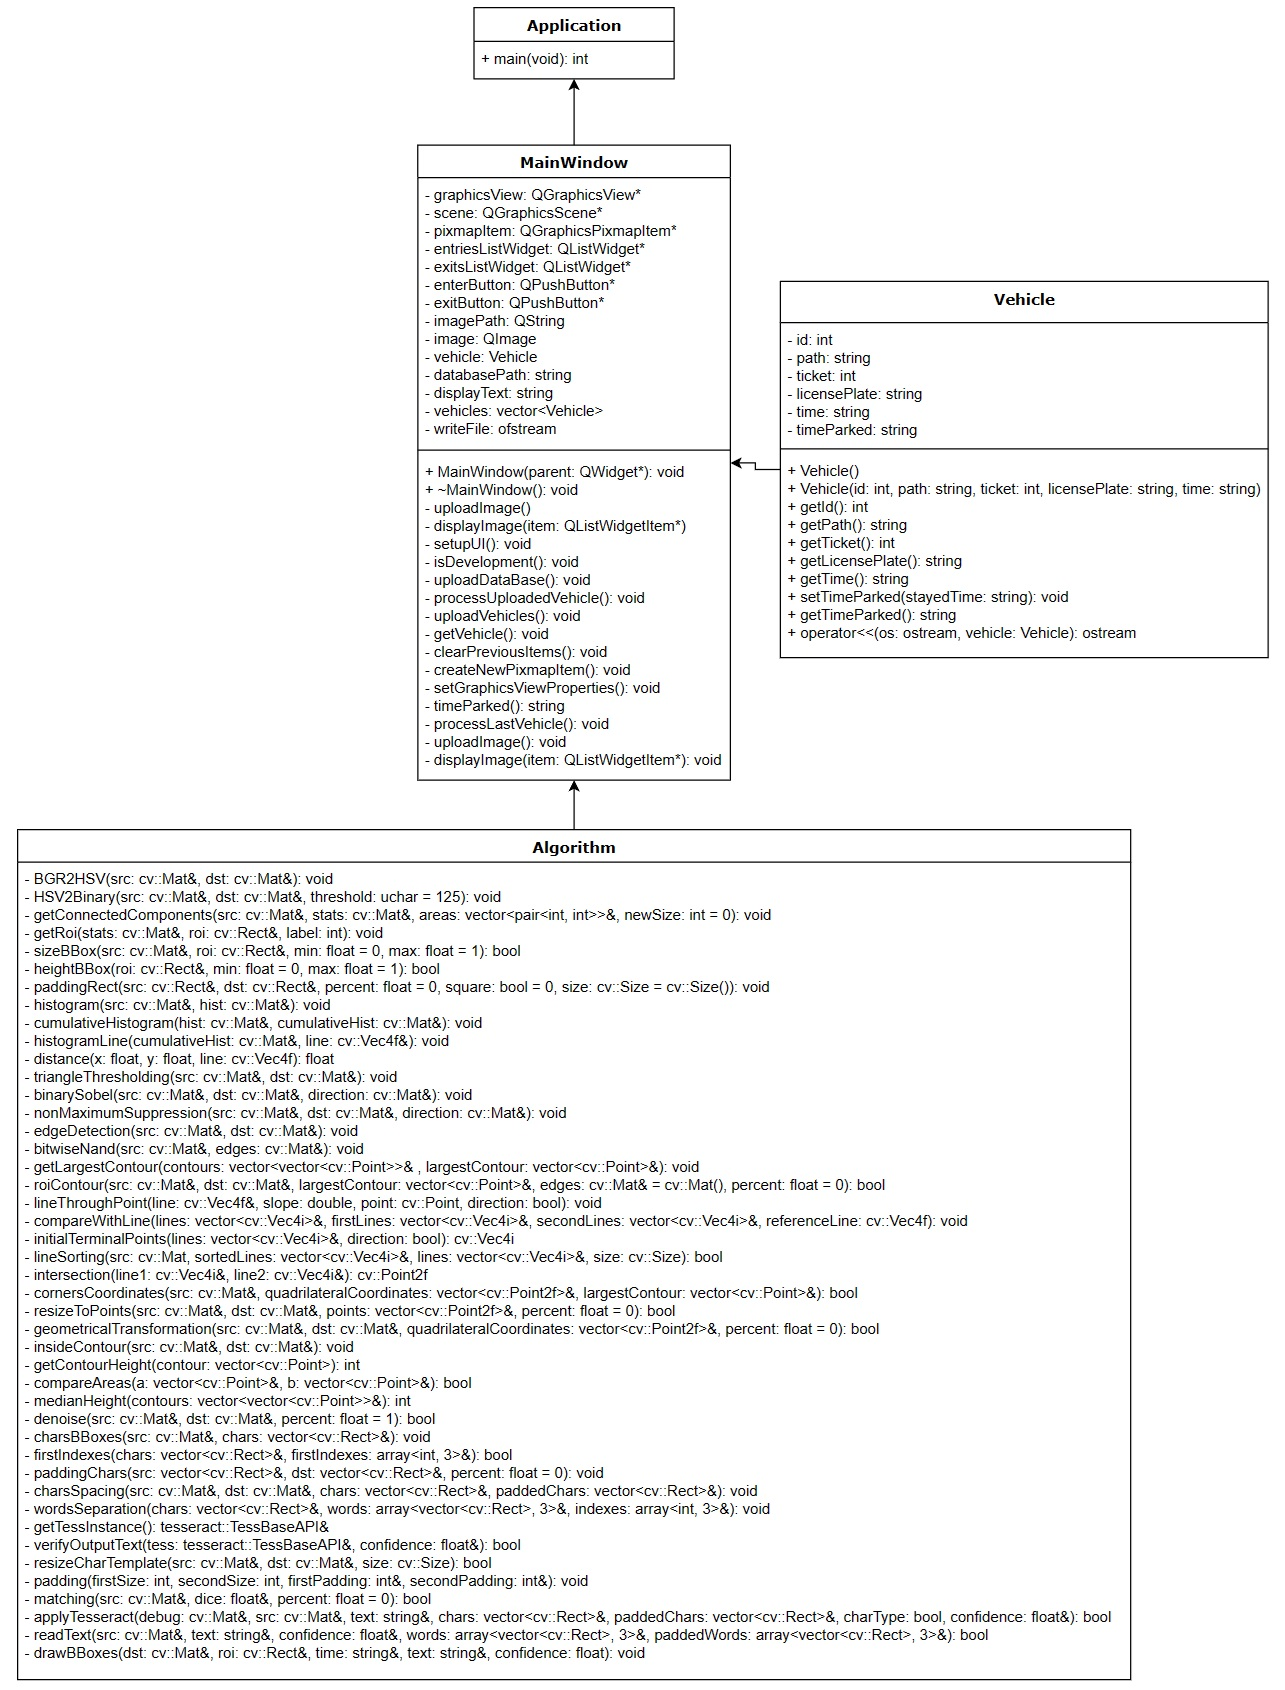
\includegraphics[width=0.7\textwidth]{images/UML.jpg}
    \caption{Diagrama UML de clase}
\end{figure}
\FloatBarrier

\section{Segmentarea, rectificarea și recunoașterea textului}
În continuare, dorim să aprofundăm pașii de execuție ai programului Toate aceste funcții se regăsesc într-o clasă denumită "Algorithm", din interiorul unei biblioteci dinamice "ImageProcessingUtils". În paralel, vom lua în considerare și o imagine drept exemplu pentru a ilustra fiecare etapă, oferind o perspectivă mai clară și mai cuprinzătoare asupra procesului de funcționare a aplicației.

\begin{figure}[h!]
    \centering
    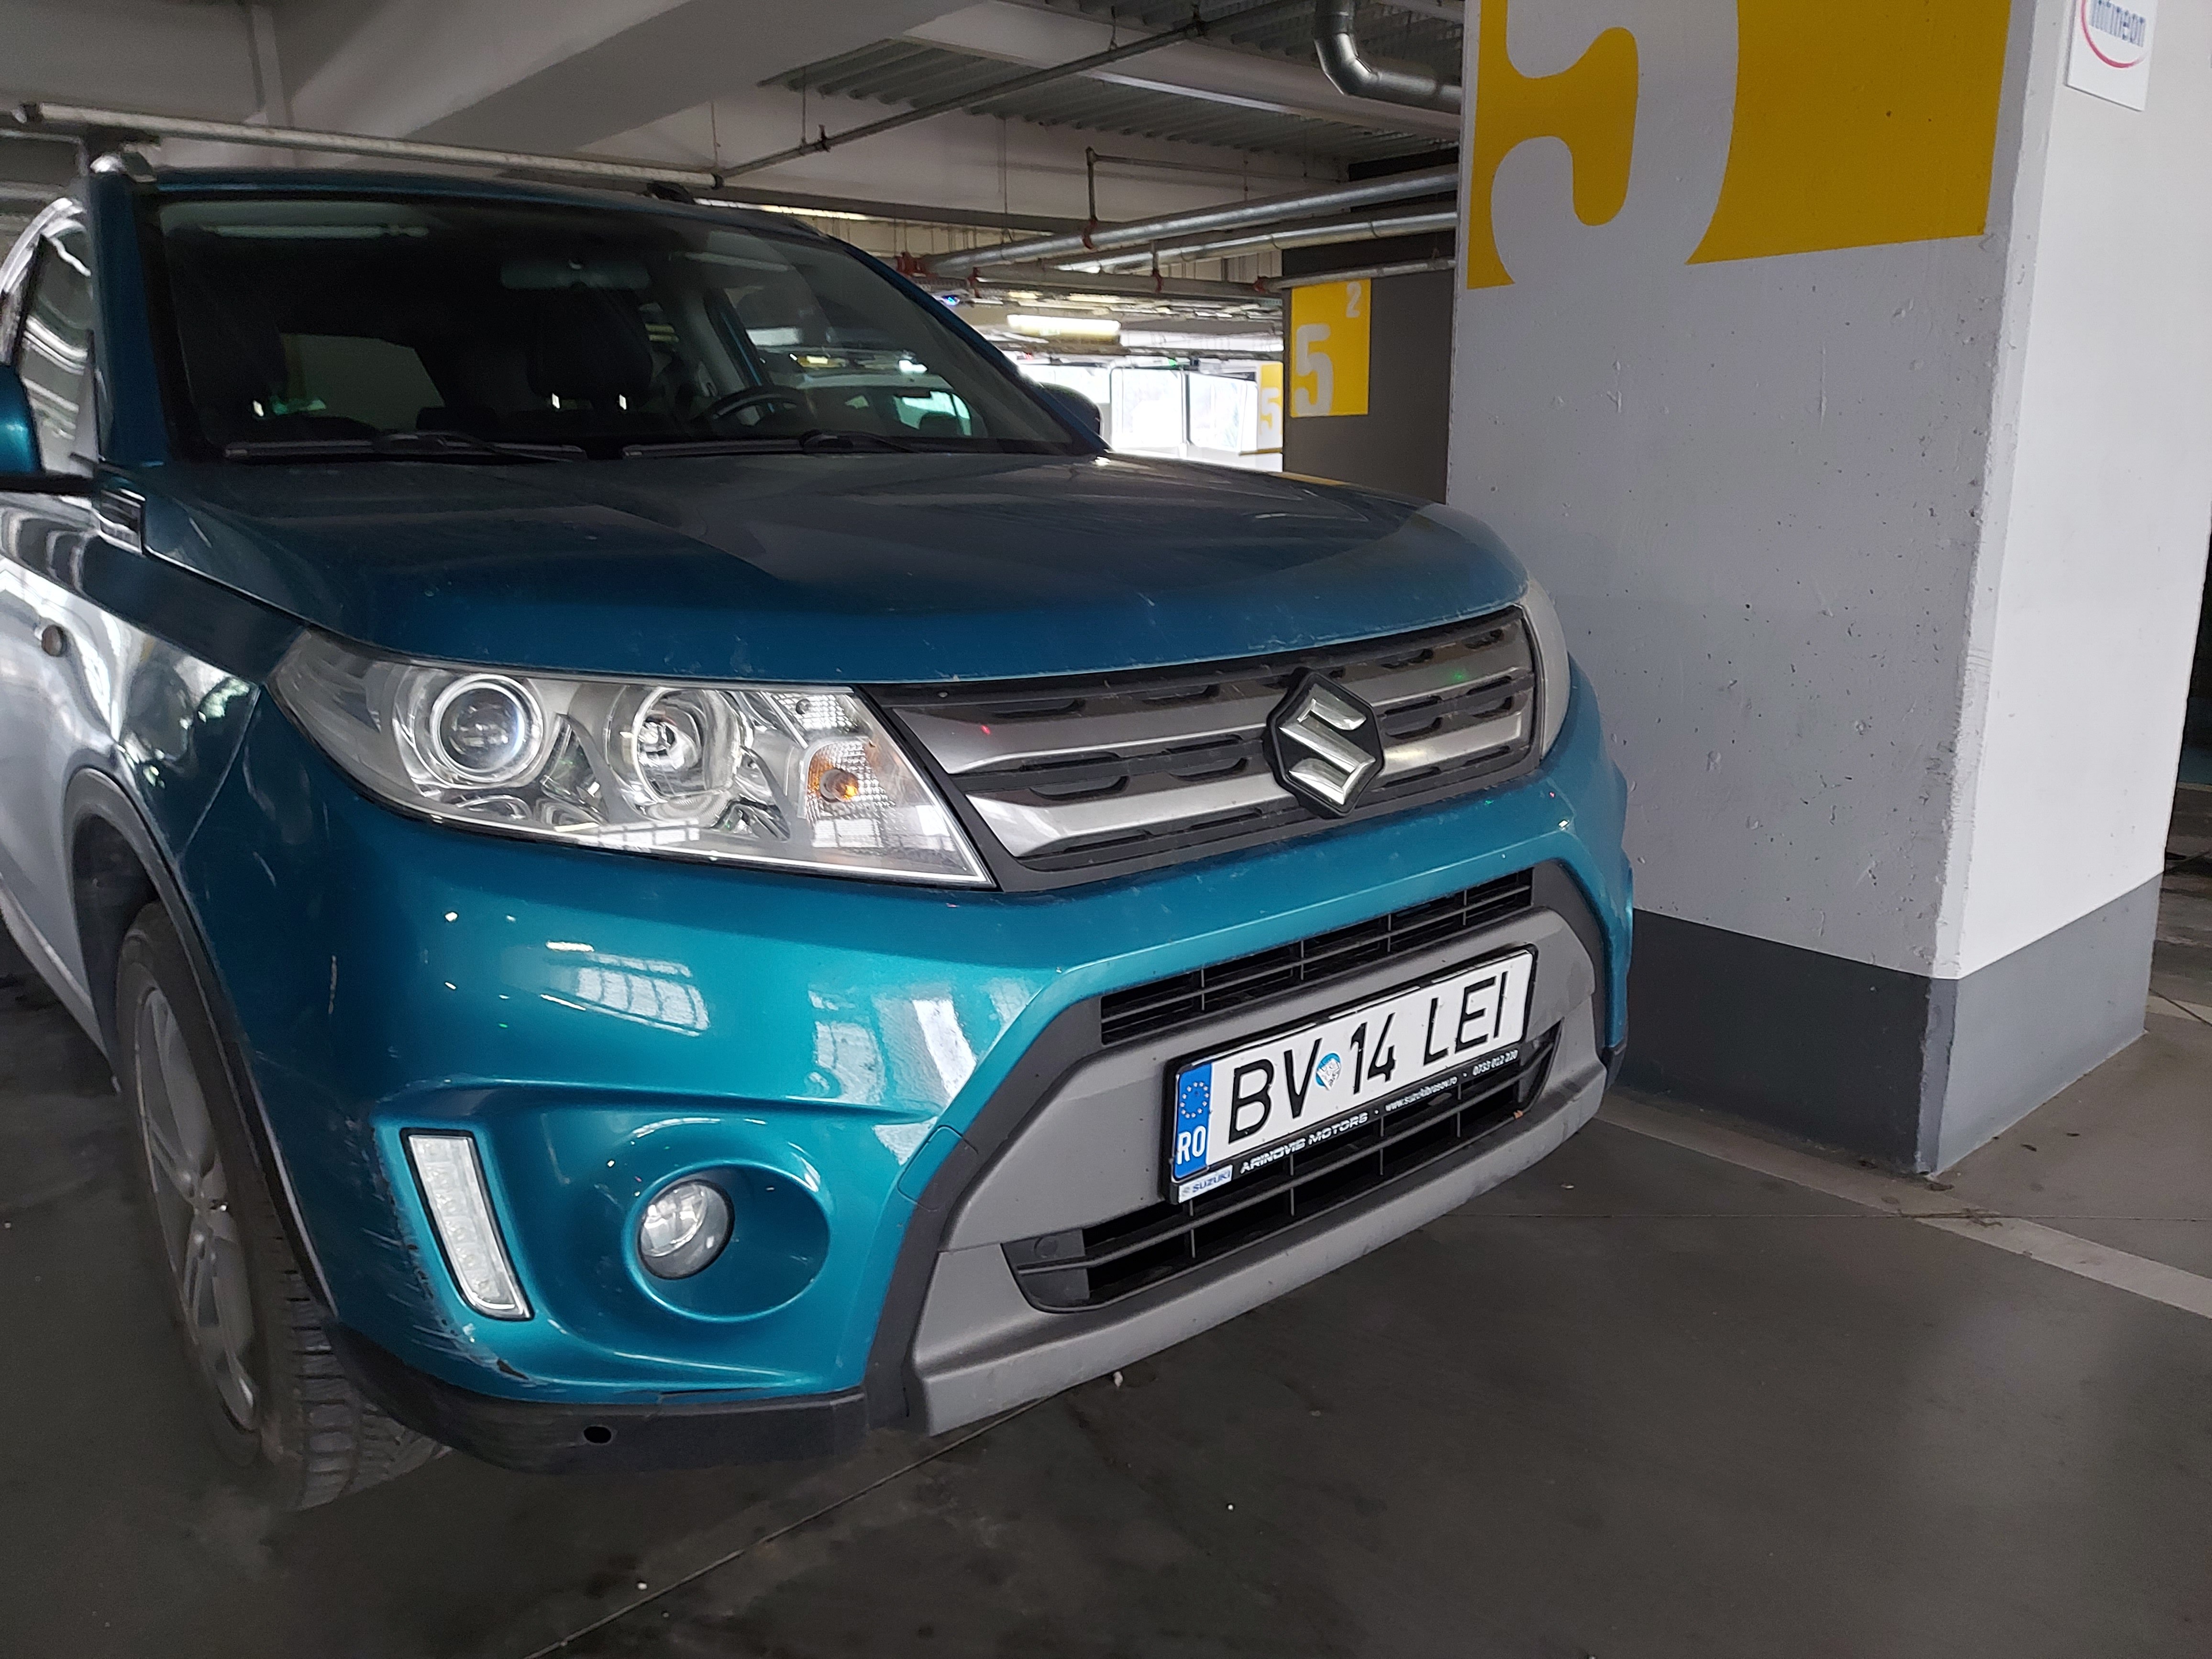
\includegraphics[width=0.4\textwidth]{images/input.jpg}
    \caption{Imaginea de input}
\end{figure}
\FloatBarrier

Pentru început, să analizăm imaginea de input. Un aspect cheie pentru program este poziționarea camerei de fotografiat, care influențează în mod direct încadrarea numărului de înmatriculare în imagine. În fotografia dată, precum și în setul de date pe care a fost testat programul, numărul de înmatriculare este situat în partea inferioară a imaginii, deoarece acesta este amplasat în general în partea de jos a vehiculelor.

Unghiul de fotografiere și distanța de la care se face poza nu influențează semnificativ procesul de segmentare, cel puțin în anumite limite. Deși, în contextul parcărilor auto, camerele de fotografiat de la intrare sunt fixate astfel încât să se obțină imagini clare din unghiuri optime, în acest exemplu, imaginea este surprinsă într-o manieră neobișnuită pentru a înțelege mai bine impactul anumitor algoritmi folosiți asupra imaginii. Acest lucru permite examinarea mai detaliată a modului în care algoritmii programului gestionează imagini cu condiții diverse de captare și încadrate atipic.

Dimensiunile imaginilor reprezintă un aspect esențial pentru performanța programului. În cazul setului de date pe care a fost testată aplicația, lucrăm cu imagini de înaltă calitate, cu o rezoluție de 4624 x 3468 x 3 și un raport de aspect de 4:3. Această dimensiune generează un număr mare de pixeli, peste 48 de milioane, ceea ce are un impact direct asupra timpului de execuție al aplicației.

Având imagini de aceste dimensiuni, este de așteptat să întâmpinăm provocări legate de viteză și eficiență. O soluție practică este redimensionarea imaginii de input la jumătate, ceea ce reduce numărul total de pixeli, menținând totuși o calitate superioară. Prin acest proces, timpul de execuție este îmbunătățit semnificativ, facilitând o procesare mai rapidă și eficientă, fără a sacrifica prea mult din calitatea imaginii. În acest fel, programul poate gestiona seturi de date mari într-un timp mai scurt, permițându-i să fie mai scalabil și să suporte un volum mai mare de procesare fără a compromite rezultatele.

Pentru a îmbunătăți timpul de execuție și mai mult, putem optimiza procesarea imaginilor concentrându-ne doar pe jumătatea inferioară a acestora. Știind că numărul de înmatriculare este de obicei amplasat în partea inferioară a vehiculului, putem decupa imaginea astfel încât să păstrăm doar jumătatea de jos a acesteia. Eventual, se pot aplica mici decupaje și din părțile laterale pentru a elimina porțiuni care nu conțin informații relevante.

\begin{figure}[h!]
    \centering
    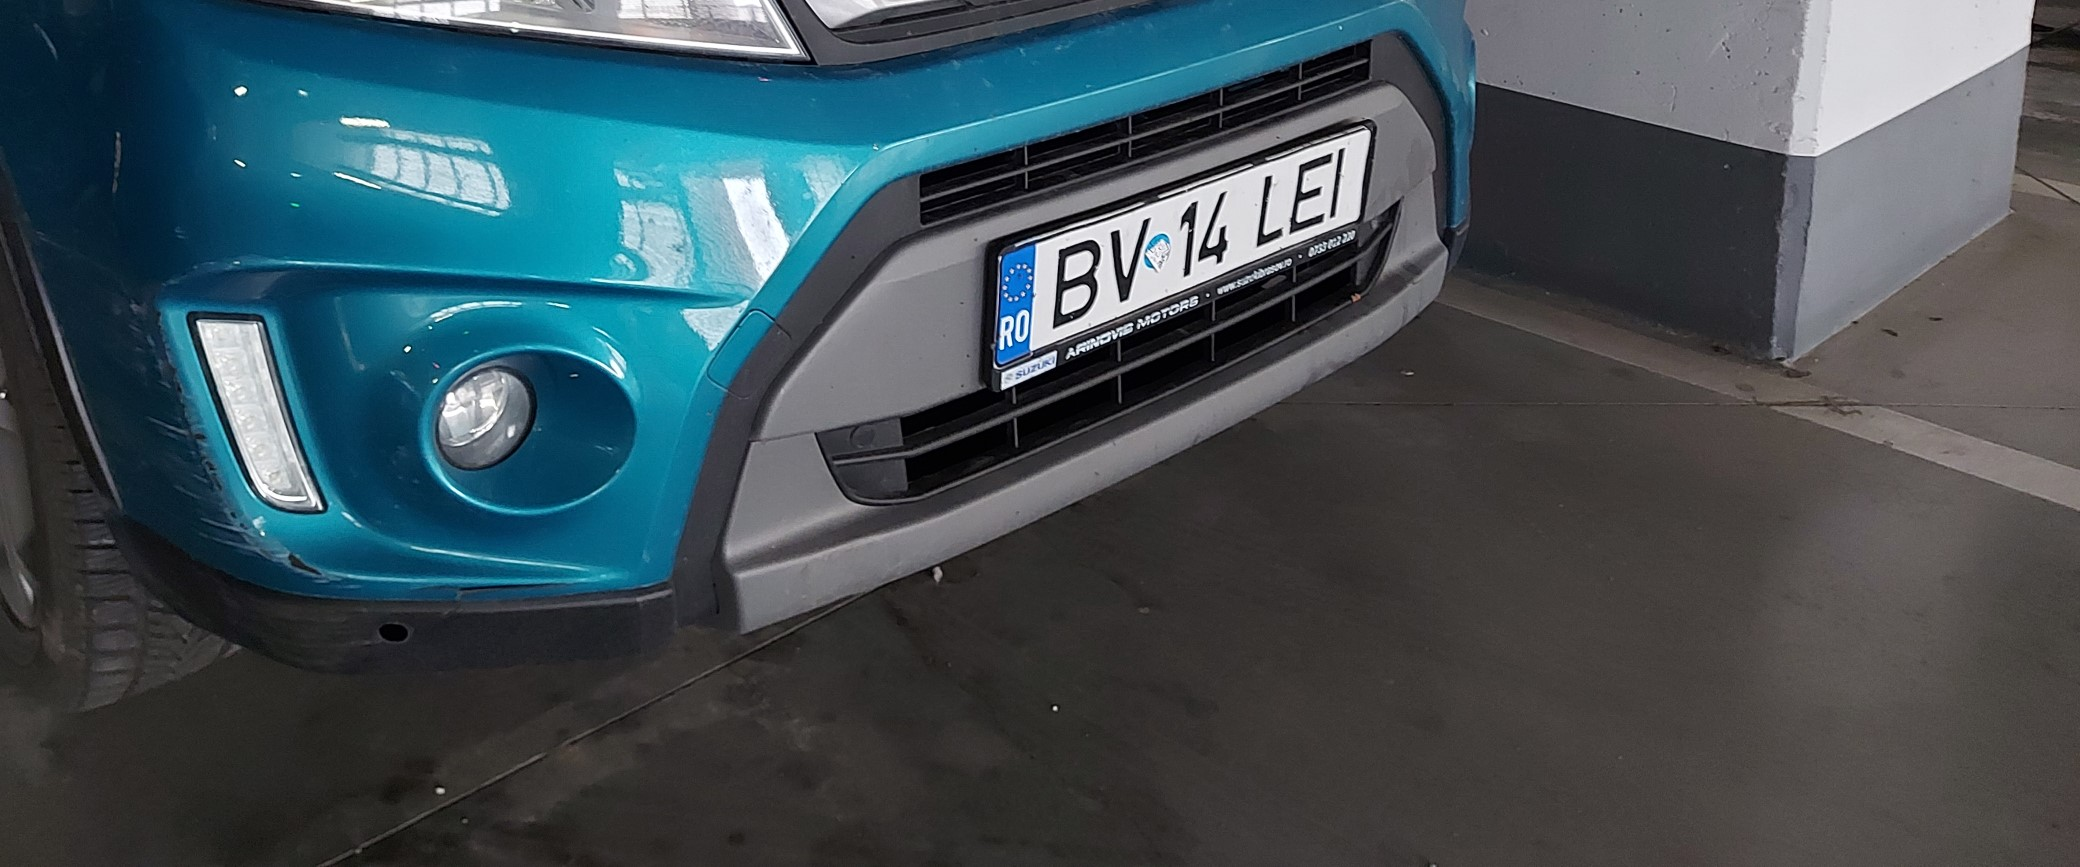
\includegraphics[width=0.4\textwidth]{images/crop.jpg}
    \caption{Partea inferioară din imaginea de input}
\end{figure}
\FloatBarrier

Această decizie are un impact direct asupra numărului de pixeli pe care algoritmii trebuie să-i proceseze, reducându-l considerabil. Cu mai puțini pixeli de analizat, timpul de execuție va fi mai rapid, iar aplicația va fi mai eficientă în procesarea imaginilor. În plus, această strategie poate ajuta la focalizarea algoritmilor pe zonele relevante ale imaginii, eliminând părțile neesențiale și reducând riscul de confuzie sau erori.

După ce imaginea a fost decupată, următorul pas este aplicarea unui filtru Gaussian pentru a elimina zgomotul generat de factori externi. Zgomotul din imagini poate apărea din diverse motive, cum ar fi condițiile de iluminare sau interferențele electronice. Filtrul Gaussian este un instrument eficient pentru reducerea zgomotului și pentru netezirea imaginii, fără a afecta contururile în mod semnificativ.

\begin{figure}[h!]
    \centering
    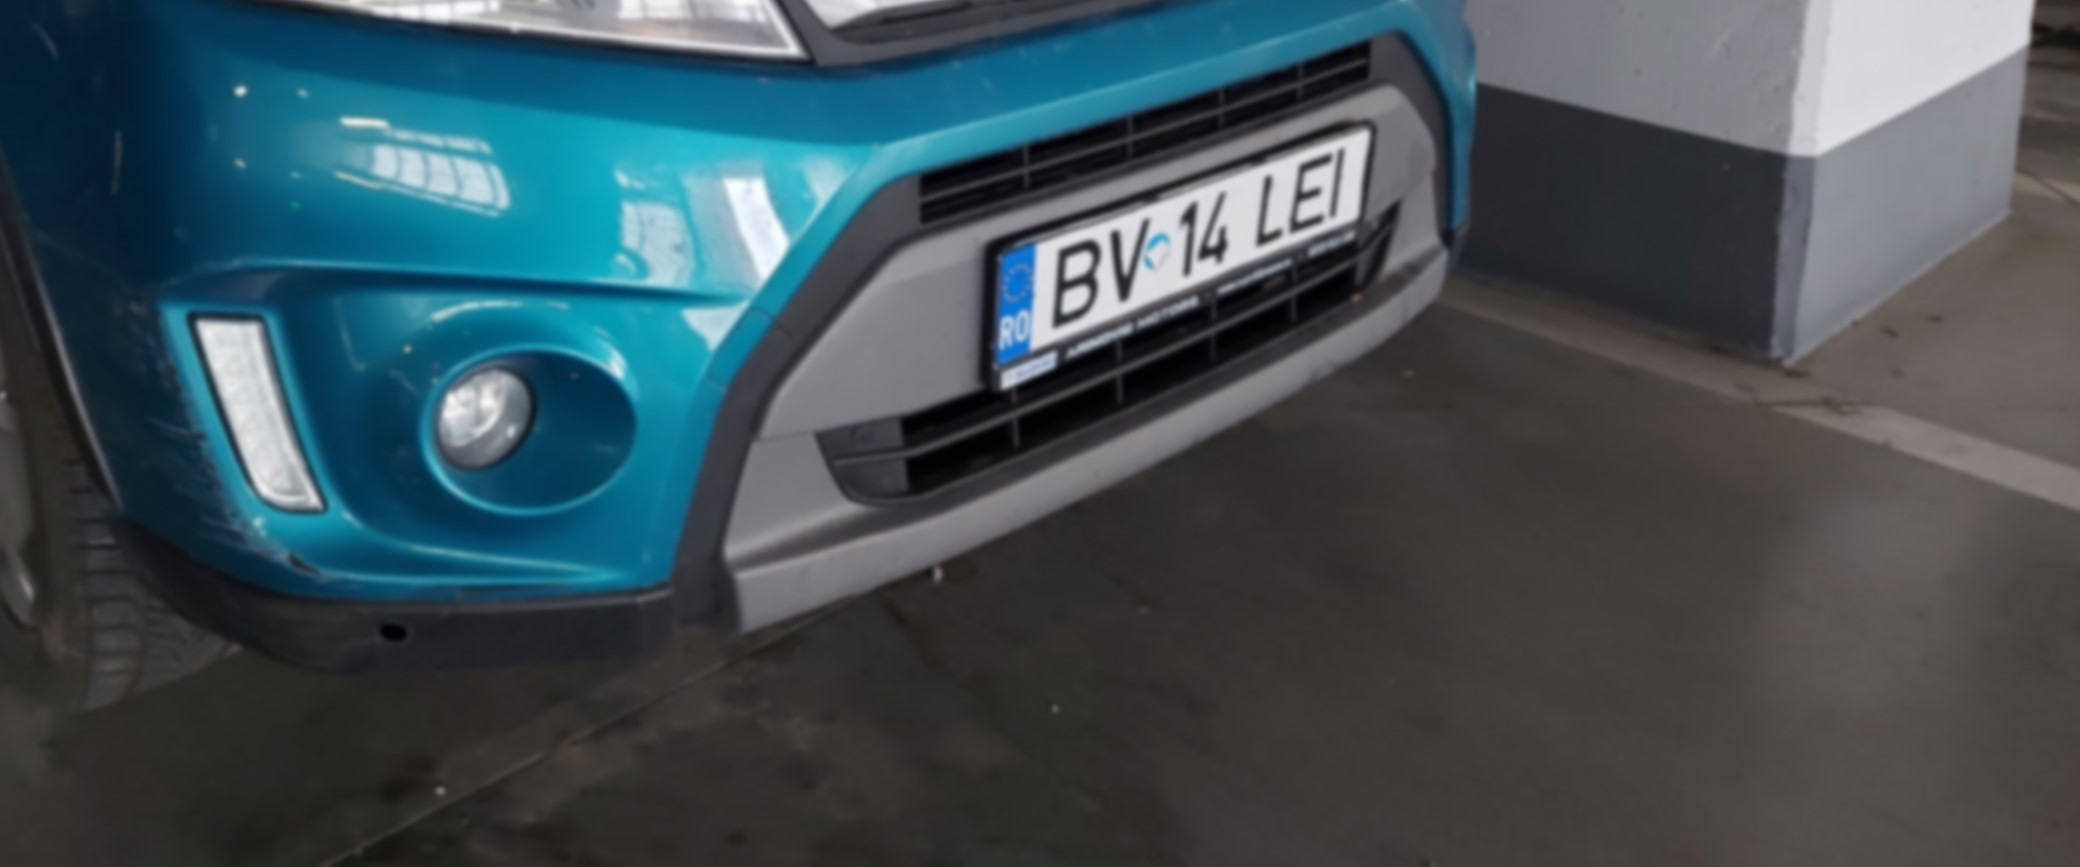
\includegraphics[width=0.4\textwidth]{images/gauss.jpg}
    \caption{Eliminarea zgomotului}
\end{figure}
\FloatBarrier

Cat despre mască, am considerat că una de dimensiune 3 x 3 este suficientă pentru imagine, întrucât nu afectează considerabil contururile așa cum ar face o mască de dimensiuni mai mari, dar totodată elimină o suficientă parte din zgomotul imaginii.

Prin aplicarea acestui filtru, imaginea decupată devine mai curată și mai ușor de procesat de algoritmi, ceea ce contribuie la rezultate mai precise. Contururile rămân clare, facilitând identificarea obiectelor sau a detaliilor importante, în timp ce zgomotul nedorit este redus semnificativ.

În următoarea etapă a procesului de prelucrare a imaginii, un pas esențial în pipeline-ul programului este binarizarea. Scopul este separarea numărului de înmatriculare de restul imaginii, iar una dintre caracteristicile cheie ale unui număr de înmatriculare este culoarea sa, care, în cazul celor din România, este albă.

Imaginile sunt de obicei reprezentate în spațiul de culoare BGR (albastru, verde, roșu), în care culoarea albă are un tuplu de valori de 255 pentru fiecare canal. Totuși, în imagini naturale, factorii externi precum vremea și lumina pot afecta culorile, astfel încât este improbabil să întâlnim albul perfect (255, 255, 255). Pentru a face procesul de binarizare mai robust, putem converti imaginea din BGR în spațiul de culoare HSV (nuanță, saturație, valoare). În acest spațiu, un obiect alb are o saturație scăzută și o valoare ridicată, în timp ce nuanța nu este un factor semnificativ.

\begin{figure}[h!]
    \centering
    \begin{minipage}{0.4\textwidth}
        \centering
        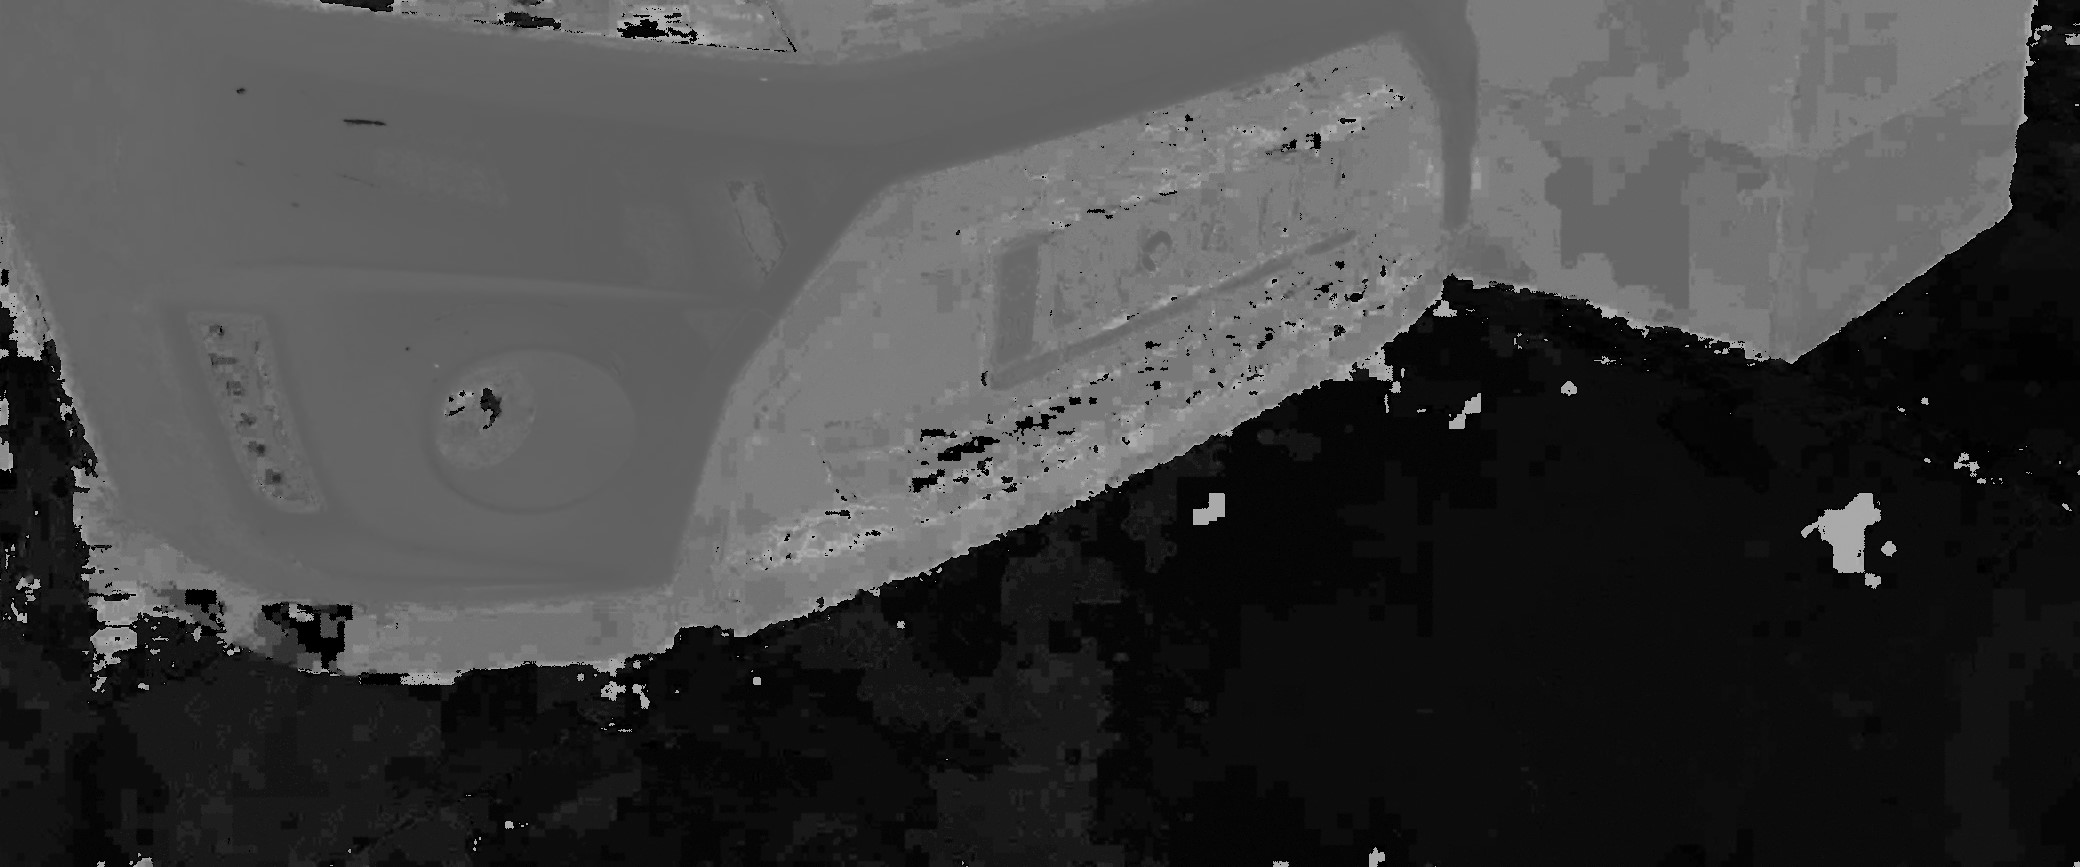
\includegraphics[width=1\textwidth]{images/hue.jpg}
        \caption{Hue (culoare)}
    \end{minipage}
    \hspace{0.05\textwidth}
    \begin{minipage}{0.4\textwidth}
        \centering
        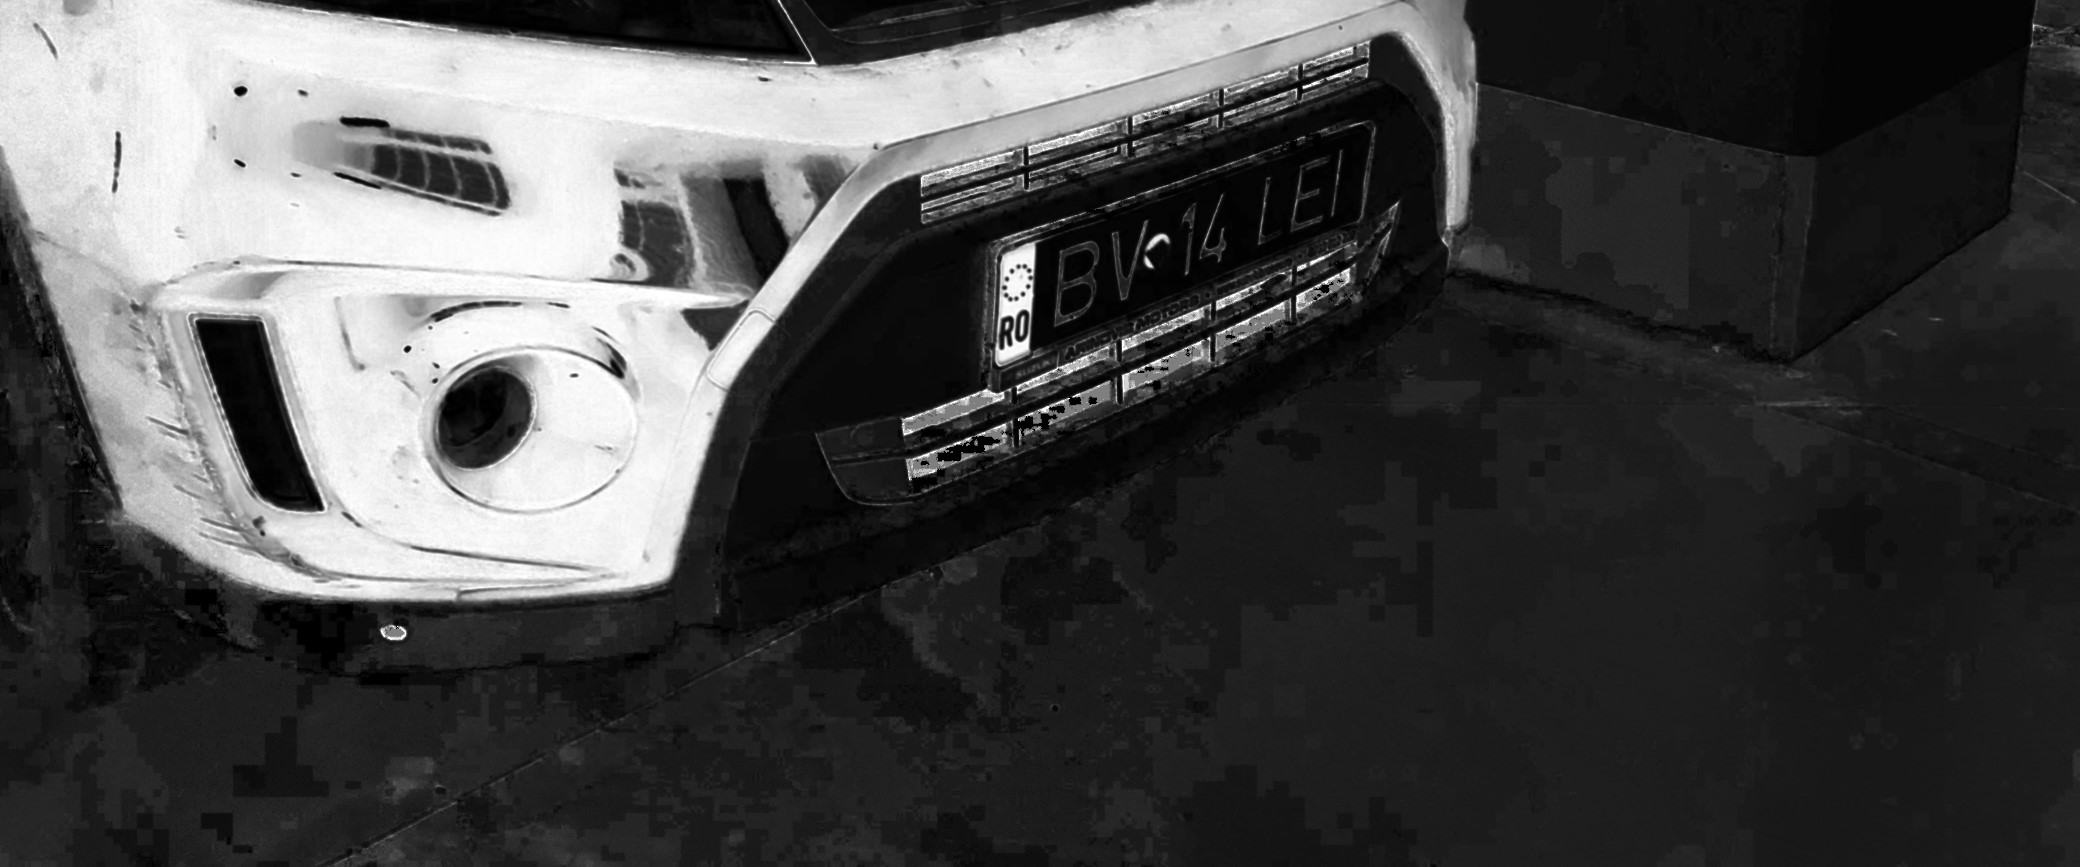
\includegraphics[width=1\textwidth]{images/saturation.jpg}
        \caption{Saturație}
    \end{minipage}
\end{figure}
\FloatBarrier
\begin{figure}[h!]
    \centering
    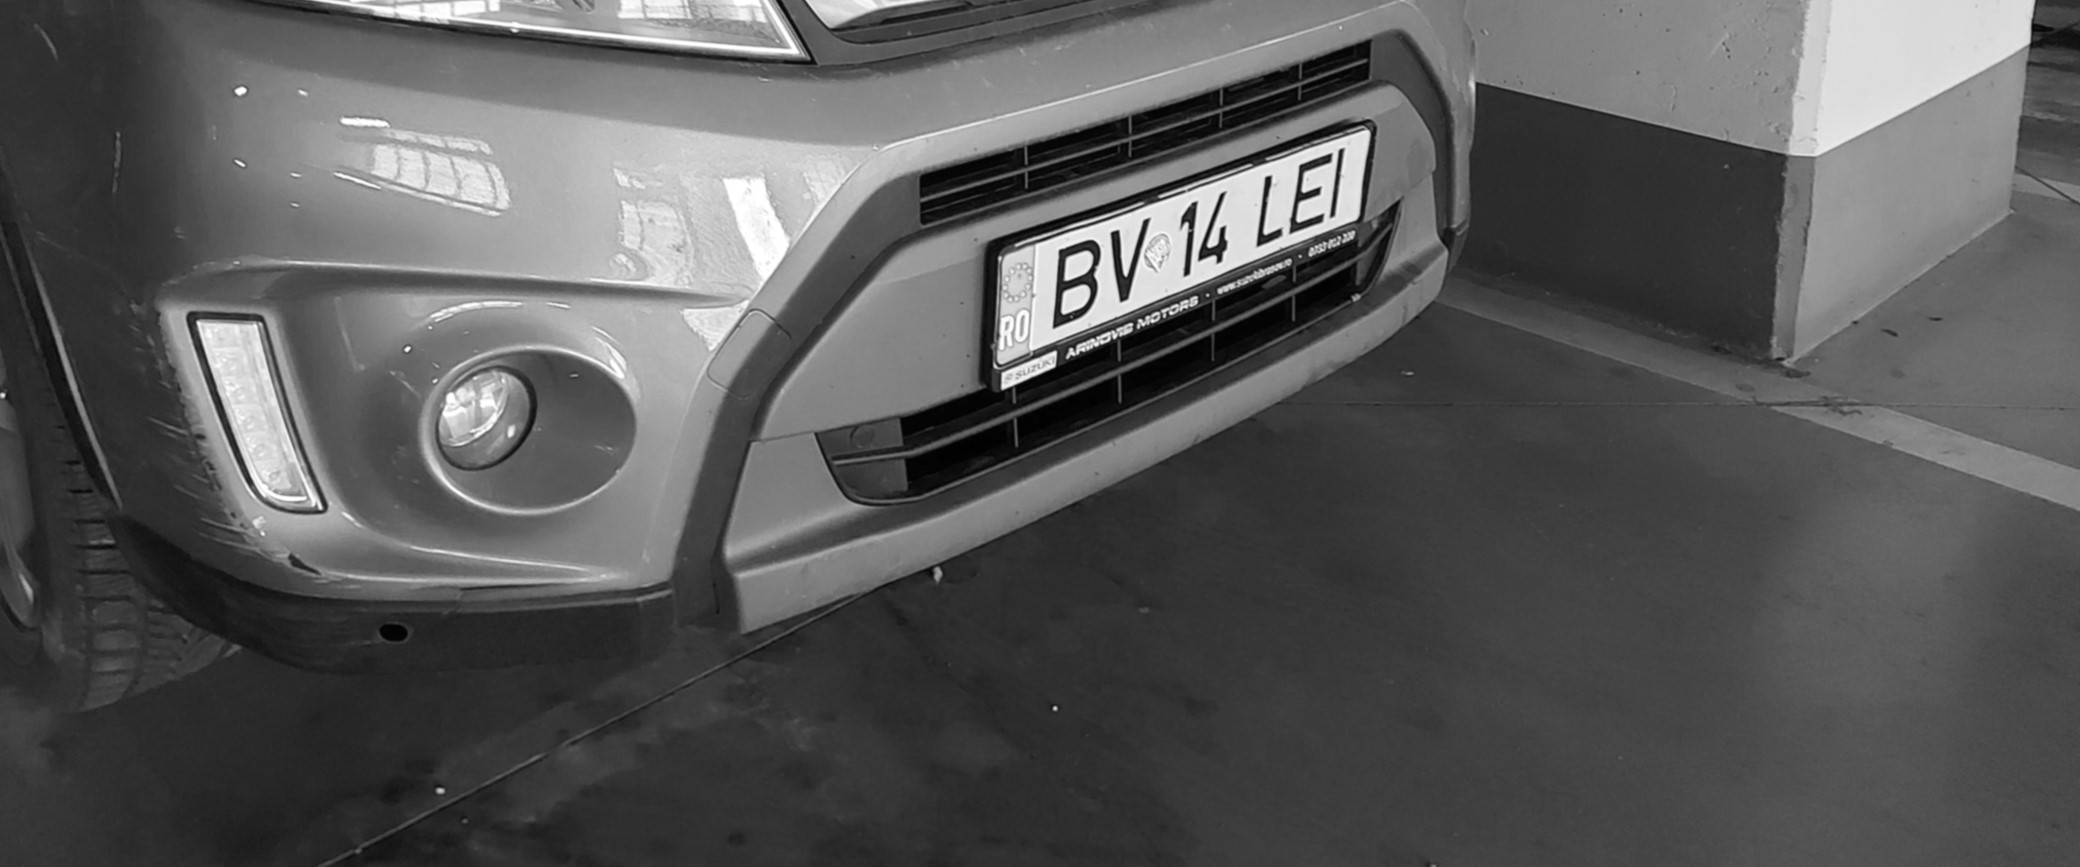
\includegraphics[width=0.4\textwidth]{images/value.jpg}
    \caption{Value (luminozitate)}
\end{figure}
\FloatBarrier

Cu imaginea convertită în spațiul HSV, putem parcurge fiecare pixel și aplica următoarea condiție: dacă pixelul are o saturație scăzută (al doilea canal) și o valoare ridicată (al treilea canal), acesta este considerat ca fiind parte a unui obiect alb, cum ar fi numărul de înmatriculare. În acest caz, pixelul este transformat în alb (255). Dacă nu îndeplinește aceste criterii, este transformat în negru (0). Această abordare creează o imagine binarizată, în care numărul de înmatriculare se va afla într-o regiune albă, față de fundalul imaginii, care va fi negru.

\begin{figure}[h!]
    \centering
    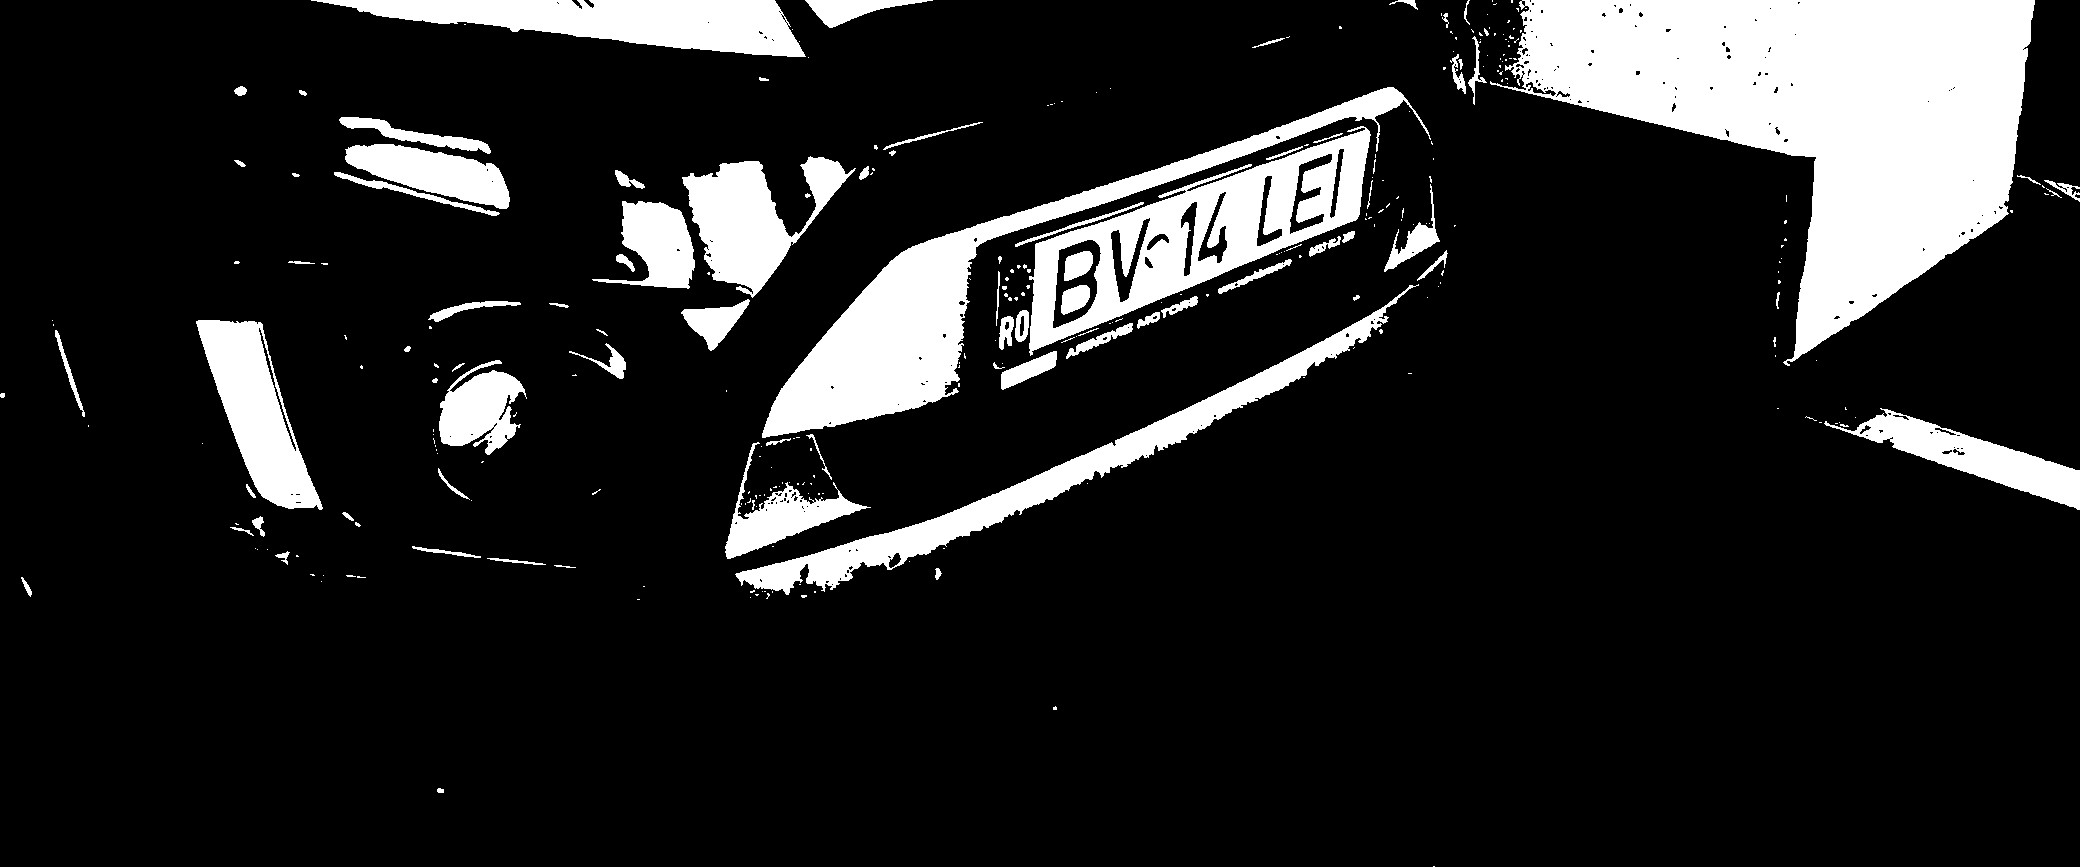
\includegraphics[width=0.4\textwidth]{images/binary.jpg}
    \caption{Imaginea de input cu filtru binar}
\end{figure}
\FloatBarrier

Următorul pas în procesul de analiză a imaginii binarizate este extragerea tuturor componentelor conexe. O componentă conexă este o mulțime de pixeli albi învecinați și conectați între ei, înconjurați la exterior de pixeli negri, cum este și cazul numărului de înmatriculare din imaginea binară. În funcție de valorile stabilite anterior ca praguri la pasul de binarizare, imaginea rezultată va avea mai multe sau mai puține componente conexe. Cu toate acestea, de cele mai multe ori, nu va conține doar componenta căutată, adică numărul de înmatriculare, ci probabil și alte componente conexe nedorite.

\begin{figure}[h!]
    \centering
    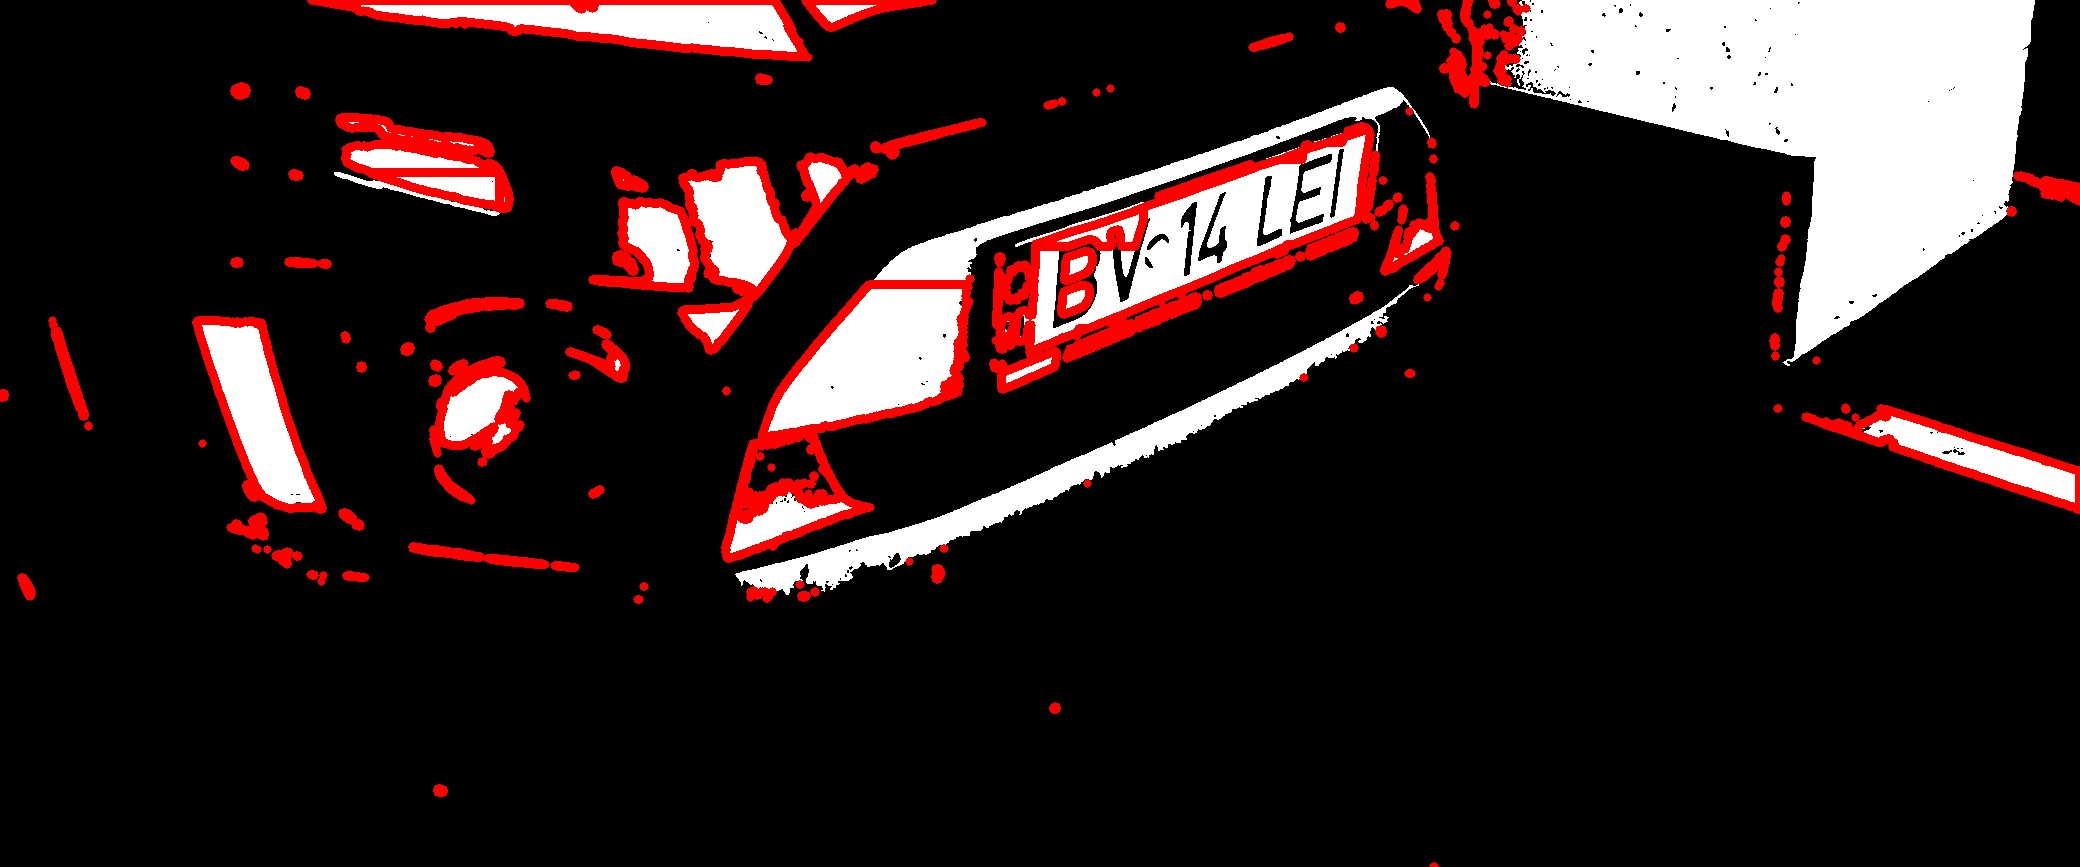
\includegraphics[width=0.4\textwidth]{images/all_connected_components.jpg}
    \caption{Conturul componentelor conexe}
\end{figure}
\FloatBarrier

Pentru a reduce din numărul componentelor conexe, putem utiliza o metodă de filtrare bazată pe dimensiunea ariei. Numărul de înmatriculare, fiind un element semnificativ în imagine, tinde să aibă o arie mai mare în comparație cu alte componente conexe. Prin urmare, putem ordona descrescător toate componentele conexe după dimensiune și să păstrăm doar primele n, unde n este stabilit în funcție de contextul imaginii. În acest exemplu, alegem n = 10, ceea ce înseamnă că rezultatul va fi un vector de dimensiune 10 care conține coordonatele colțului din stânga sus ale fiecărei componente conexe, precum și înălțimea și lățimea fiecărei componente.

\begin{figure}[h!]
    \centering
    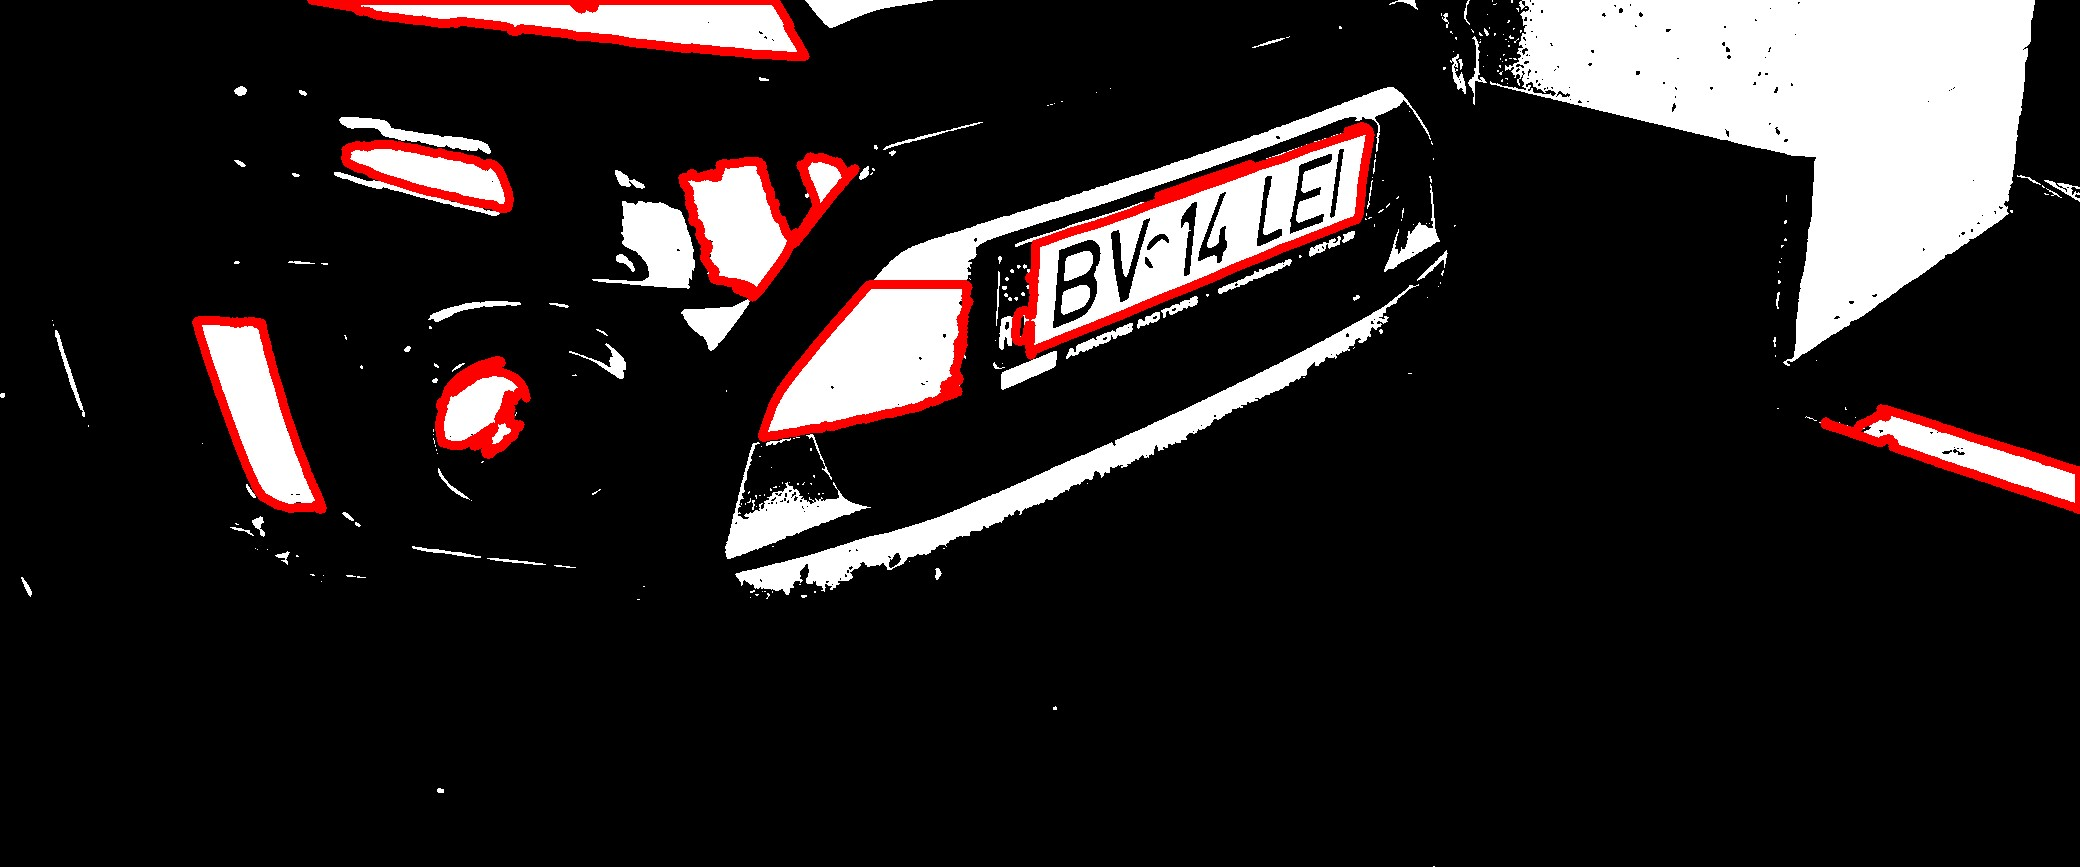
\includegraphics[width=0.4\textwidth]{images/connected_components.jpg}
    \caption{Conturul celor mai mari 10 componente conexe}
\end{figure}
\FloatBarrier

Pentru a identifica componenta conexă ce conține numărul de înmatriculare, vom face segmentări din imagine, numite și regiuni de interes (ROI), pe baza vectorului rezultat, și vom analiza fiecare regiune obținută, care încadrează câte o componentă conexă. Știm că un număr de înmatriculare are o formă dreptunghiulară, cu o înălțime mică în comparație cu lățimea și cu o arie destul de mică în raport cu întreaga imagine. Pe baza acestor informații, putem stabili condiții pentru a filtra componentele conexe și a ne concentra pe cea care ar putea corespunde unui număr de înmatriculare.

\begin{figure}[h!]
    \centering
    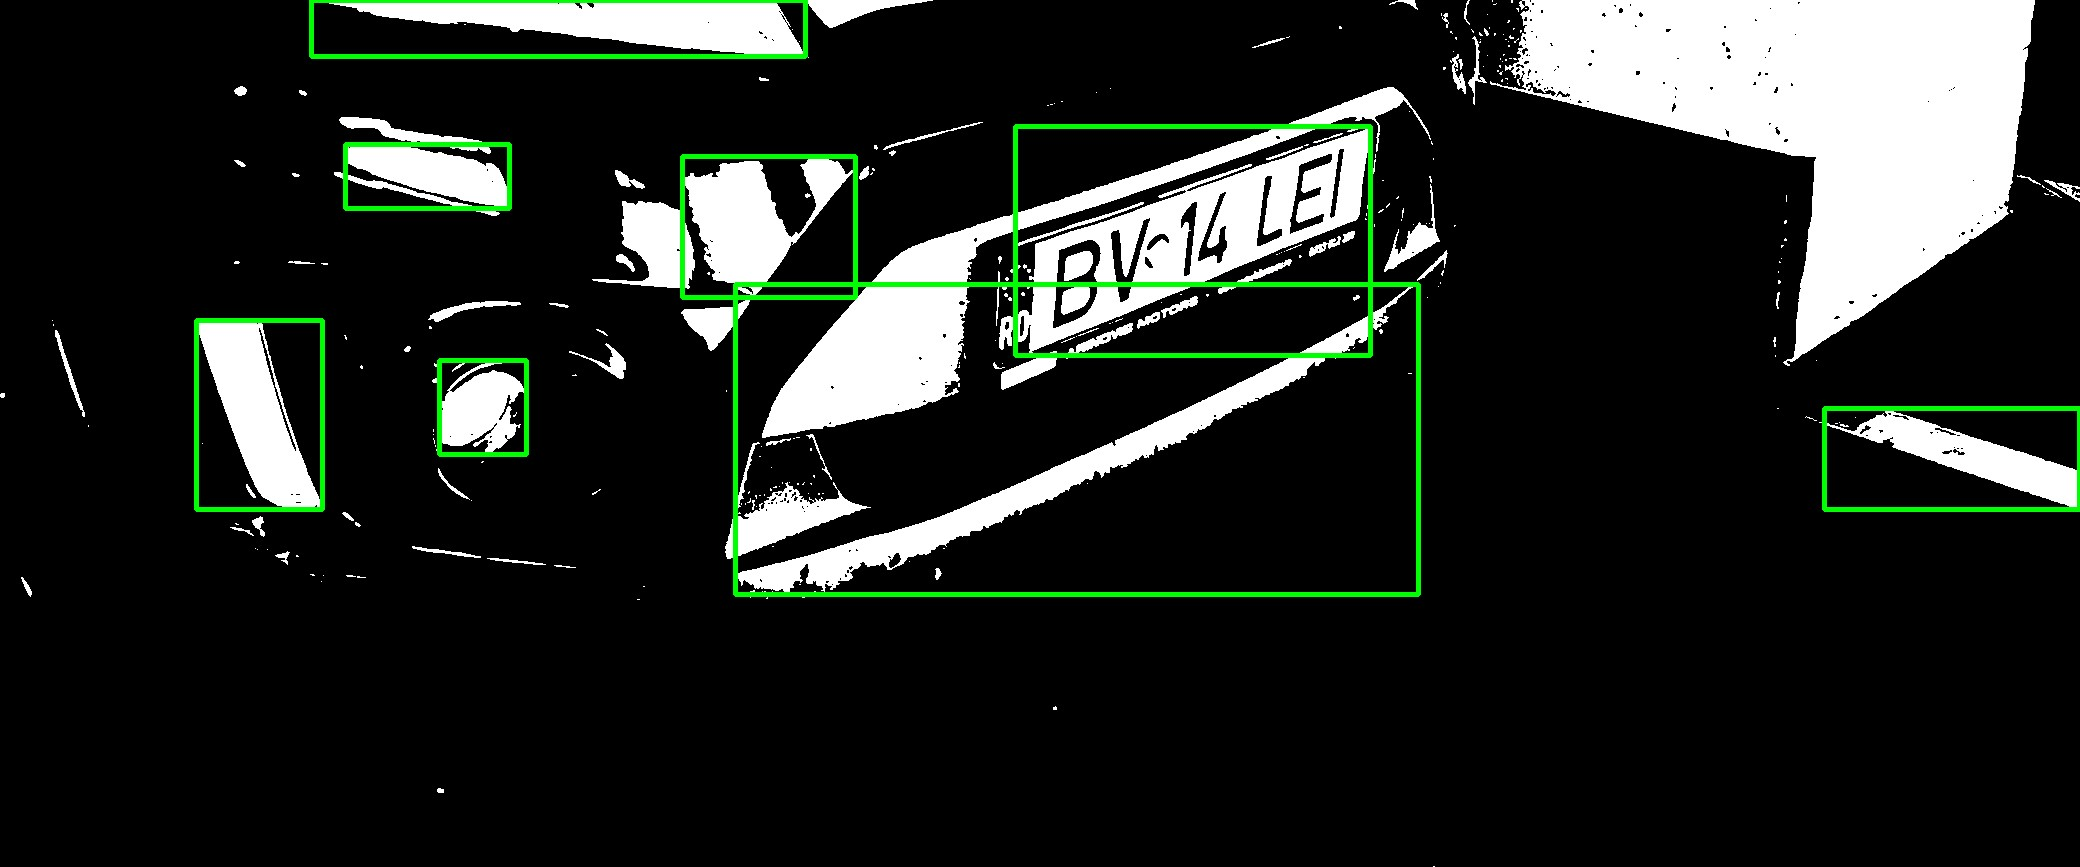
\includegraphics[width=0.4\textwidth]{images/bboxes.jpg}
    \caption{Bounding box-urile componentelor conexe}
\end{figure}
\FloatBarrier

O condiție importantă pentru selecție este raportul dintre înălțimea și lățimea regiunii de interes. Pentru a se califica ca potențial candidat pentru numărul de înmatriculare, înălțimea segmentării trebuie să fie mai mare decât un anumit procent din lățimea acesteia, dar nu mai mare decât un alt procent. De exemplu, putem stabili că înălțimea trebuie să fie între 20\% și 90\% din lățime, permițând o flexibilitate suficientă pentru a include numerele de înmatriculare care ar putea fi înclinate, rezultând forme aproape pătratice.

\[
    ROI.height \in [ROI.width \times min, \ ROI.width \times max]; \, min, \ max \in [0, 1]
\]

Dacă această condiție este îndeplinită, următorul pas este calcularea ariei regiunii de interes și compararea acesteia cu aria totală a imaginii. Pentru a se califica, aria trebuie să fie între anumite limite procentuale, de exemplu, între 1\% și 15\% din aria totală.

\[
    ROI.area \in [Sursa.area \times min, \ Sursa.area \times max]; \, min, \ max \in [0, 1]
\]

Acest proces de filtrare bazat pe aspectul dreptunghiular și dimensiunea ariei ajută la reducerea numărului de componente conexe care nu reprezintă numere de înmatriculare, asigurând că ne concentrăm pe candidații cei mai probabili. În plus, flexibilitatea condițiilor permite ajustări în funcție de imagini cu numere de înmatriculare în poziții variabile sau înclinate.

\begin{figure}[h!]
    \centering
    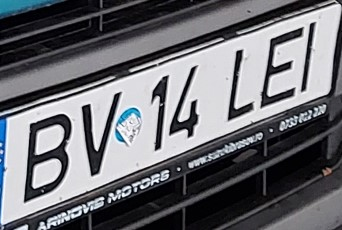
\includegraphics[width=0.4\textwidth]{images/color_roi.jpg}
    \caption{Segmentarea din imaginea de input}
\end{figure}
\FloatBarrier

Acum că regiunea de interes (ROI) pare să aibă dimensiuni similare cu un număr de înmatriculare, putem aplica diferiți algoritmi pentru a detecta contururile, care vor fi folosiți în pașii următori ai programului. Începem prin adăugarea unui padding la regiunea noastră de interes pentru a asigura continuitatea contururilor, evitând astfel întreruperi cauzate de dimensiunile măștilor utilizate pentru detectarea marginilor. Padding-ul este important pentru a ne asigura că niciun pixel relevant nu este omis în zonele limită.

\begin{figure}[h!]
    \centering
    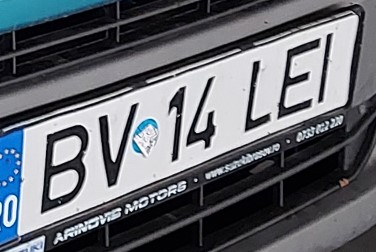
\includegraphics[width=0.4\textwidth]{images/padded_roi.jpg}
    \caption{Imaginea segmentată cu padding adăugat}
\end{figure}
\FloatBarrier

După aceasta, convertim segmentarea în format grayscale, deoarece algoritmii de detectare a marginilor necesită imagini în tonuri de gri.

\begin{figure}[h!]
    \centering
    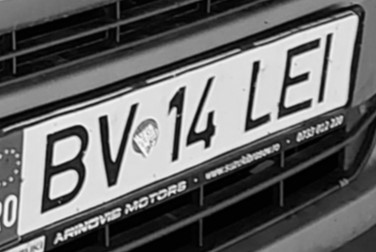
\includegraphics[width=0.4\textwidth]{images/gray_roi.jpg}
    \caption{Imaginea segmentată in format grayscale}
\end{figure}
\FloatBarrier

Primul pas este aplicarea filtrului Sobel, care detectează marginile bazându-se pe derivata imaginii. Pentru a obține o binarizare clară, aplicăm un filtru de binarizare Triangular Thresholding pentru a păstra doar pixelii relevanți detectați de Sobel, care sunt cu adevărat contururi.

\begin{figure}[h!]
    \centering
    \begin{minipage}{0.4\textwidth}
        \centering
        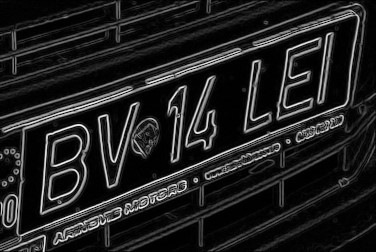
\includegraphics[width=1\textwidth]{images/sobel.jpg}
        \caption{Filtru Sobel}
    \end{minipage}
    \hspace{0.05\textwidth}
    \begin{minipage}{0.4\textwidth}
        \centering
        
\includegraphics[width=1\textwidth]{images/binary_sobel.jpg}
        \caption{Filtru Sobel binarizat cu metoda Triangle Thresholding}
    \end{minipage}
\end{figure}
\FloatBarrier

Pentru a ne asigura că am captat toți pixelii relevanți din imagine, aplicăm și un filtru de obținere a gradientului morfologic tot pe regiunea în format grayscale, urmat de încă un filtru de binarizare Triangular Thresholding. Astfel, avem două imagini binare: una cu rezultatele filtrului Sobel și alta cu gradientul morfologic.

\begin{figure}[h!]
    \centering
    \begin{minipage}{0.4\textwidth}
        \centering
        
\includegraphics[width=1\textwidth]{images/gradient.jpg}
        \caption{Gradienții morfologici}
    \end{minipage}
    \hspace{0.05\textwidth}
    \begin{minipage}{0.4\textwidth}
        \centering
        
\includegraphics[width=1\textwidth]{images/binary_gradient.jpg}
        \caption{Gradienții morfologici binarizati cu metoda Triangle Thresholding}
    \end{minipage}
\end{figure}
\FloatBarrier

Următorul pas este combinarea acestor două imagini binare, păstrând în imaginea cu gradienții morfologici doar acei pixeli care apar în cel puțin una dintre imaginile binare.

\begin{figure}[h!]
    \centering
    \begin{minipage}{0.4\textwidth}
        \centering
        
\includegraphics[width=1\textwidth]{images/or_binary.jpg}
        \caption{Reuniunea celor doua imagini binare (masca)}
    \end{minipage}
    \hspace{0.05\textwidth}
    \begin{minipage}{0.4\textwidth}
        \centering
        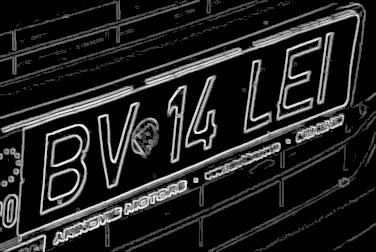
\includegraphics[width=1\textwidth]{images/or_gradient.jpg}
        \caption{Gradienții morfologici dupa mască}
    \end{minipage}
\end{figure}
\FloatBarrier

Acum, că avem doar pixelii care ar putea aparține unor contururi, aplicăm un filtru de subțiere Non-Maximum Suppression pentru a obține margini de un pixel grosime, astfel încât contururile să fie clare și precise.

\begin{figure}[h!]
    \centering
    
\includegraphics[width=0.4\textwidth]{images/non_maximum_suppression.jpg}
    \caption{Edge map de un pixel grosime}
\end{figure}
\FloatBarrier

În următorul pas, revenim la regiunea de interes în formatul grayscale și aplicăm un filtru de binarizare automatizat, cum ar fi Triangle Thresholding sau Otsu. Segmentarea este un dreptunghi în care ar trebui să fie inclus numărul de înmatriculare (dacă este regiunea corectă), dar în acesta pot exista și alte elemente din imaginea inițială care nu ne interesează.

\begin{figure}[h!]
    \centering
    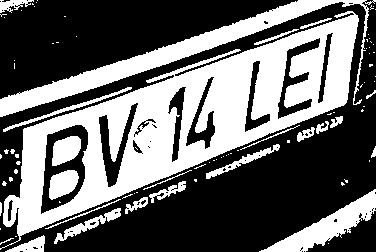
\includegraphics[width=0.4\textwidth]{images/before_roi.jpg}
    \caption{Imaginea segmentată cu filtru binar}
\end{figure}
\FloatBarrier

După aplicarea filtrului de binarizare, în imagine ar trebui observat un chenar alb care conține literele și cifrele numărului de înmatriculare și care ar trebui să fie separat de restul imaginii. Acum putem căuta din nou componentele conexe și păstra strict pe cea de dimensiunea cea mai mare, care ar trebui să fie chenarul alb. Însă pot apărea situații în care această binarizare este eronată și chenarul alb este conectat cu alte zone formate din pixeli albi.

Pentru a corecta acest lucru, folosim edge map-ul obținut anterior. Știm că în edge map contururile sunt reprezentate ca pixeli de valoare 255, deci putem verifica că pixelii albi (255) din edge map sunt negri (0) în regiunea binarizată. Acest lucru asigură că pixelii contururilor rămân separați și nu conectează eronat zonele între ele.

\begin{figure}[h!]
    \centering
    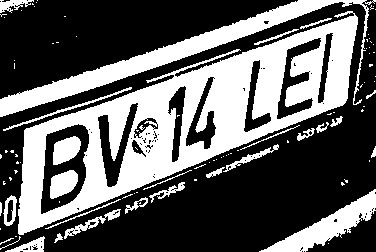
\includegraphics[width=0.4\textwidth]{images/after_roi.jpg}
    \caption{Corecția imaginii segmentate}
\end{figure}
\FloatBarrier

Pentru a fi complet siguri că nu există legături incorecte, putem aplica o operație morfologică de tip Opening. Această operație separă obiectele legate incorect prin linii fine.

După operația de Opening, este posibil să apară noi componente conexe, deci aplicăm din nou căutarea componentelor conexe și păstrăm doar componenta de dimensiunea cea mai mare. Aceasta ar trebui să fie chenarul alb care conține numărul de înmatriculare.

\begin{figure}[h!]
    \centering
    
\includegraphics[width=0.4\textwidth]{images/roi.jpg}
    \caption{Regiunea textului}
\end{figure}
\FloatBarrier

Pentru a reduce numărul de segmente și pentru a ne apropia de regiunea care conține numărul de înmatriculare, putem adăuga o nouă condiție pentru imaginea segmentată, care ar trebui să conțină numai zona textului numărului de înmatriculare. Această condiție stabilește că înălțimea zonei respective ar trebui să fie aproape egală cu întreaga înălțime a imaginii de segmentare. Prin urmare, putem compara înălțimea acestei zone cu un procentaj, să zicem 80\%, din înălțimea regiunii de interes pentru a valida corectitudinea segmentării.
\[
    width > ROI.width \times percent; \, percent \in [0, 1]
\]

În pasul de rectificare, trebuie să obținem 4 coordonate pe baza cărora se va face rectificarea, aceste 4 coordonate fiind chiar colțurile chenarului alb în care se află numărul de înmatriculare. Pentru început, scădem din imaginea sursă imaginea sursă erodată pentru a obține exact conturul chenarului alb. Pe imaginea rezultată putem aplica algoritmul Hough, care ne va returna liniile din imagine, din intersectarea cărora putem obține coordonatele colțurilor.

\begin{figure}[h!]
    \centering
    
\includegraphics[width=0.4\textwidth]{images/edges.jpg}
    \caption{Conturul regiunii}
\end{figure}
\FloatBarrier

Pentru a face acest lucru, primul pas este să stabilim parametrii funcției Hough. Doi parametri importanți din funcția Hough sunt lungimea minimă admisă pentru o linie ca aceasta să fie adăugată ca rezultat și distanța maximă dintre două linii ca acestea să fie considerate de fapt aceeași linie, dar cu o întrerupere eronată între ele, și astfel în vectorul rezultat, în loc de două linii, să fie adăugată una singură formată din aceste două. Valorile acestor doi parametri sunt obținute în mod automatizat pe baza bounding box-ului rotit.

\begin{figure}[h!]
    \centering
    \includegraphics[width=0.4\textwidth]{images/rotated_rect.jpg}
    \caption{Bounding box-ul rotit al regiunii}
\end{figure}
\FloatBarrier

Având acest bounding box în care componenta conexă este încadrată exact, putem estima dimensiunile acesteia, deci și dimensiunile liniilor Hough. Astfel, pentru lungimea minimă a liniilor și distanța maximă dintre acestea, vom considera anumite procente din înălțimea bounding box-ului. Totuși, aceste procente pot fi destul de mici, de exemplu, 30\% pentru lungimea minimă a liniilor și 15\% pentru distanța maximă dintre acestea.

Această abordare este necesară deoarece, cu cât unghiul de fotografiere este mai inclinat, cu atât și numărul de înmatriculare va fi mai înclinat în imagine. În astfel de cazuri, algoritmul Hough, în loc să detecteze puține linii de dimensiuni mari, detectează multe linii de dimensiuni mici. Astfel, dacă stabilim valori mari parametrilor funcției, multe linii nu vor fi luate în calcul când numărul de înmatriculare este mai inclinat. Chiar și așa, dacă în continuare nu am obținut toate liniile de care aveam nevoie, putem decrementa treptat lungimea minimă a acestora, pentru a obține în final mai multe linii.

\begin{figure}[h!]
    \centering
    \includegraphics[width=0.4\textwidth]{images/lines.jpg}
    \caption{Liniile Hough}
\end{figure}
\FloatBarrier

Liniile de care avem nevoie sunt câte una din fiecare parte a chenarului alb, mai exact partea de sus, jos, stânga, dreapta, pentru că mai apoi să le putem găsi punctele de intersectie. Însă, algoritmul Hough nu ne oferă și informația de care parte aparține fiecare linie, așa că următoarea etapă este o sortare. Pentru început, vom sorta liniile ca fiind verticale sau orizontale. Putem obține această informație în funcție de panta fiecărei drepte:
\[
    slope = \frac{y_2 - y_1}{x_2 - x_1}
\]

Unghiul de înclinare se calculează apoi astfel:
\[
    angle = \lvert \arctan(slope) \times \frac{180}{\pi} \rvert
\]

Deci, dacă unghiul este aproape de 0 grade, linia este considerată orizontală, iar dacă este aproape de 90 de grade, linia este considerată verticală. Trebuie să ținem cont și de cazurile în care panta este complet verticală, pentru a evita împărțirea la zero.

\begin{figure}[h!]
    \centering
    \includegraphics[width=0.4\textwidth]{images/horizontal_vertical_lines.jpg}
    \caption{Separarea liniilor verticale și orizontale}
\end{figure}
\FloatBarrier

După sortarea liniilor în verticale și orizontale, putem identifica liniile de care avem nevoie pentru fiecare parte a chenarului alb: partea de sus, jos, stânga, dreapta. Pentru a face acest lucru, luăm ca referință o linie verticală și una orizontală prin centrul imaginii, față de care se compară și se clasifică fiecare linie detectată de algoritmul Hough.

\begin{figure}[h!]
    \centering
    \includegraphics[width=0.4\textwidth]{images/reference_lines.jpg}
    \caption{Liniile de comparație}
\end{figure}
\FloatBarrier

În trasarea celor două linii de referință, vom ține cont și de pante, cel puțin în cazul celei orizontale, deoarece numărul de înmatriculare poate fi inclinat la un unghi atât de mare încât unele linii să fie clasificate eronat. În cazul în care numărul de înmatriculare este inclinat la un anumit unghi, și liniile trasate prin centrul imaginii trebuie să fie inclinate la unghiul respectiv pentru a se face clasificarea într-un mod corect.

După ce avem vectorii cu liniile orizontale și verticale, putem să-i parcurgem și să comparăm fiecare linie cu liniile de referință pentru a determina orientarea lor. Linia verticală de referință este utilizată pentru a compara liniile verticale, iar linia orizontală de referință pentru cele orizontale.

Pentru a face această comparație, putem folosi formula distanței dintre două drepte:
\[
    distance = (x - x_1) \cdot (y_2 - y_1) - (y - y_1) \cdot (x_2 - x_1)
\]

Semnul distanței ajută să separăm liniile detectate. Cele de deasupra liniei de referință vor avea distanțe pozitive, iar cele de dedesubt vor avea distanțe negative. La fel, liniile din dreapta vor avea distanțe pozitive față de linia de referință verticală, iar cele din stânga vor avea distanțe negative.

\begin{figure}[h!]
    \centering
    \includegraphics[width=0.4\textwidth]{images/multiple_lines.jpg}
    \caption{Clasificarea Liniile Hough}
\end{figure}
\FloatBarrier

Ideal, rezultatul ar trebui să fie compus din patru linii, câte una pentru fiecare parte a chenarului alb. Cu toate acestea, din cauza erorilor de detectare sau a înclinațiilor, pot apărea mai multe segmente în loc de o singură linie. Dacă avem mai multe segmente, putem căuta capetele cele mai îndepărtate în funcție de orientare pentru a le lega între ele și a obține o singură linie pentru fiecare parte.

\begin{figure}[h!]
    \centering
    \includegraphics[width=0.4\textwidth]{images/sorted_lines.jpg}
    \caption{Cele 4 linii rezultate}
\end{figure}
\FloatBarrier

Acesta este și momentul în care verificăm dacă trebuie să aplicăm din nou algoritmul Hough cu parametrii ajustați sau dacă am găsit toate liniile necesare. Dacă avem cele patru linii căutate, pasul următor este să calculăm punctele de intersecție între ele pentru a obține coordonatele colțurilor chenarului alb. Ordinea este următoarea:
\begin{itemize}
    \item Punctul din stânga sus se obține prin intersectarea liniei din stânga cu cea de sus.
    \item Punctul din dreapta sus se obține prin intersectarea liniei din dreapta cu cea de sus.
    \item Punctul din dreapta jos se obține prin intersectarea liniei din dreapta cu cea de jos.
    \item Punctul din stânga jos se obține prin intersectarea liniei din stânga cu cea de jos.
\end{itemize}

\begin{figure}[h!]
    \centering
    \includegraphics[width=0.4\textwidth]{images/points.jpg}
    \caption{Punctele de rectificare}
\end{figure}
\FloatBarrier

O problemă des întâlnită cu liniile detectate este că punctele de intersecție pot fi în afara imaginii, ceea ce necesită un padding suficient de mare pentru a cuprinde toate cele patru puncte de intersecție. Pentru a rezolva această situație, trebuie să căutăm coordonatele cele mai mici și cele mai mari pentru X și Y dintre punctele calculate anterior:
\[
    \begin{aligned}
        minX & = ROI.width, \, minY = ROI.height, \ maxX = 0, \, maxY = 0,
    \end{aligned}
\]
Pentru fiecare punct (\(x, y\)):
\[
    \begin{aligned}
        minX & = \min(minX, x); \\
        minY & = \min(minY, y); \\
        maxX & = \max(maxX, x); \\
        maxY & = \max(maxY, y).
    \end{aligned}
\]

După ce avem aceste valori, putem calcula dimensiunea padding-ului necesar pentru fiecare parte a imaginii. Dacă punctele de intersecție sunt în afara imaginii, vom ajusta padding-ul pentru a le include:
\[
    \begin{aligned}
        paddingRight  & = \max(0, maxX - (src.cols - 1)), \\
        paddingBottom & = \max(0, maxY - (src.rows - 1)), \\
        paddingLeft   & = \max(0, -minX),                 \\
        paddingTop    & = \max(0, -minY).
    \end{aligned}
\]

Această abordare ne permite să ajustăm imaginea astfel încât toate punctele de intersecție să fie incluse în limitele acesteia, inclusiv punctele care au coordonate mai mari decât dimensiunile imaginii inițiale. Însă, dacă există și puncte cu coordonate negative pentru care a fost adăugat padding în partea de sus a imaginii sau în partea din stânga, suntem nevoiți să ajustăm toate punctele de intersecție cu valoarea padding-ului adăugat pentru a reflecta noua poziție în cadrul imaginii extinse:

Pentru fiecare punct (\(x, y\)):
\[
    \begin{aligned}
        x = paddingLeft + x, \\
        y = paddingTop + y.
    \end{aligned}
\]

Acum că avem cele patru coordonate ale colțurilor chenarului alb și ne-am asigurat că sunt în interiorul imaginii, putem trece la pasul de rectificare. Rectificarea presupune transformarea geometrică a regiunii de interes pentru a alinia numărul de înmatriculare într-o poziție corectă, obținând astfel o imagine rectificată.

Pentru a începe procesul de rectificare, calculăm dimensiunile imaginii rezultate. Pentru a determina înălțimea corectă a numărului de înmatriculare, scădem coordonata Y a punctului din stânga sus din coordonata Y a punctului din stânga jos:
\[
    height = DownLeft.y - UpLeft.y
\]

Pentru a obține lățimea, folosim raportul cunoscut pentru numărul de înmatriculare, unde lățimea este de 4.3 ori mai mare decât înălțimea:
\[
    width = 4.3 \times height
\]

Cu aceste dimensiuni calculate, putem stabili punctele corespunzătoare pentru fiecare colț al chenarului alb în imaginea destinată. Ordinea punctelor pentru colțurile chenarului alb este: stânga sus, dreapta sus, dreapta jos, stânga jos. Pentru imaginea rectificată, punctele corespondente vor fi:
\begin{itemize}
    \item (0, 0) pentru stânga sus,
    \item (width - 1, 0) pentru dreapta sus,
    \item (width - 1, height - 1) pentru dreapta jos,
    \item (0, height - 1) pentru stânga jos.
\end{itemize}

\begin{figure}[h!]
    \centering
    \includegraphics[width=0.4\textwidth]{images/points_on_black.jpg}
    \caption{Punctele de rectificare in imaginea destinație}
\end{figure}
\FloatBarrier

Cu aceste puncte corespondente, putem calcula matricea de transformare utilizând funcția de transformare geometrică. Aplicând această transformare pe imaginea segmentată în formatul grayscale, obținem în final numărul de înmatriculare într-o formă rectificată.

\begin{figure}[h!]
    \centering
    \includegraphics[width=0.4\textwidth]{images/transformed.jpg}
    \caption{Imaginea rectificată}
\end{figure}
\FloatBarrier

Imaginea rezultată ar trebui să conțină literele și cifrele numărului de înmatriculare pe fundal alb. Însă, există și situații în care rectificarea nu este tocmai ideală, iar astfel pot apărea diverse probleme: anumite caractere nu sunt în totalitate incadrate în imagine, iar astfel, spre exemplu, un caracter este ușor tăiat într-o parte anume, sau, în cazul opus, zona rectificată este ușor mai mare și astfel se obțin detalii în plus la extremitățile imaginii, detalii ce nu sunt necesare.

Ca o primă soluție este decuparea de pe fiecare parte a imaginii a câte o linie sau a câte o coloană, ca mai apoi să se adauge un padding alb în locul liniilor și coloanelor decupate. Decupând o mică parte din imagine, se reduce din posibila zonă care este în plus. De asemenea, padding-ul alb de jur împrejurul imaginii asigură că nu va exista un contur discontinuu al chenarului alb, cum s-ar întâmpla în cazul în care o literă nu este întru totul încadrată în imagine și întrerupe conturul dreptunghiular al chenarului.

\begin{figure}[h!]
    \centering
    \includegraphics[width=0.4\textwidth]{images/boardered.jpg}
    \caption{Imaginea rectificată cu padding adăugat}
\end{figure}
\FloatBarrier

Următorul pas este aplicarea unui filtru Binary Thresholding pe imaginea rectificată. Acest lucru va crea o imagine binarizată în care literele și cifrele numărului de înmatriculare vor fi separate de fundal. Însă, se aplică și un filtru de inversare a culorilor deoarece caracterele sunt de culoare neagră pe un fundal alb, pe când acestea ar trebui să fie albe pe un fundal negru.

\begin{figure}[h!]
    \centering
    \includegraphics[width=0.4\textwidth]{images/text.jpg}
    \caption{Imaginea rectificată cu filtru binar}
\end{figure}
\FloatBarrier

Caracterele numărului de înmatriculare pot fi considerate și componente conexe în imaginea binară. De asemenea, știm că numerele de înmatriculare în formatul din România au între 6 și 8 caractere, deci tot atâtea componente conexe trebuie să existe în imaginea binară. Însă, nu este întotdeauna așa, căci uneori numărul de înmatriculare poate avea diferite însemnări pe care le vom considera artefacte și pe care dorim să le eliminăm.

O primă etapă este detectarea tuturor componentelor conexe din imagine și ordonarea acestora după aria lor. Cele mai mari componente conexe tind să fie caracterele numărului de înmatriculare. După ordonare, păstrăm primele opt componente, deoarece, așa cum am stabilit, un număr de înmatriculare nu are mai mult de opt caractere.

\begin{figure}[h!]
    \centering
    \includegraphics[width=0.4\textwidth]{images/before_denoise.jpg}
    \caption{Primele 8 componente conexe}
\end{figure}
\FloatBarrier

Cu toate acestea, tot este posibil ca una sau două componente conexe din imagine să fie de fapt zgomot. Pentru a detecta și elimina posibilul zgomot, putem folosi înălțimea ca un factor comun între caractere. Calculăm înălțimea mediană a componentelor conexe și o folosim ca referință pentru a compara înălțimea fiecărei componente cu cea mediană:
\[
    \left| median - height \right| > median \times percent; \, percent \in [0, 1]
\]

Dacă diferența dintre înălțimea componentei conexe curente și cea mediană este mai mare decât un anumit procent din înălțimea mediană, de exemplu 20\%, putem considera acea componentă ca fiind zgomot și se elimină. Prin aplicarea acestui filtru bazat pe înălțime, ne putem asigura că imaginea finală conține doar componentele conexe care corespund literelor și cifrelor numărului de înmatriculare.

\begin{figure}[h!]
    \centering
    \includegraphics[width=0.4\textwidth]{images/after_denoise.jpg}
    \caption{Eliminarea componentelor conexe eronate}
\end{figure}
\FloatBarrier

De asemenea, ca la un pas anterior, pentru a fi complet siguri că nu există legături incorecte între componentele conexe, putem aplica și o operație morfologică de tip Opening. Această operație separă obiectele legate incorect prin linii fine.

După operația de Opening, este posibil să apară noi componente conexe, motiv pentru care se aplică din nou funcția descrisă anterior și astfel se elimină noile componente conexe, care nu sunt caractere, rezultate din urma operației morfologice.

În urma aplicării tuturor tehnicilor de procesare a imaginilor, am obținut o imagine în care textul numărului de înmatriculare arată ca și cum ar fi fost tastat manual într-un fișier. Aceasta este o imagine potrivită pentru modelul de recunoaștere a caracterelor Tesseract OCR. Totuși, pentru a obține rezultate mai bune, este util să furnizăm modelului AI fiecare caracter separat, pe rând.

Pentru a realiza acest lucru, aplicăm pe imaginea binară rectificată funcția implementată într-un pas anterior ce detectează componentele conexe, pentru a obține bounding box-urile tuturor caracterelor. Rezultatul este din nou un vector ce conține coordonatele colțului din stânga sus ale fiecărui bounding box, precum și înălțimea și lățimea fiecărei componente. Este important să cunoaștem ordinea corectă a caracterelor în imagine pentru a putea reconstrui textul numărului de înmatriculare din caracterele recunoscute.

\begin{figure}[h!]
    \centering
    \includegraphics[width=0.4\textwidth]{images/chars.jpg}
    \caption{Bounding box-urile caracterelor}
\end{figure}
\FloatBarrier

Cu toate acestea, ordinea în care componentele conexe sunt stocate în vector poate să nu coincidă cu ordinea reală a caracterelor în imagine. Pentru a remedia acest lucru, sortăm vectorul în ordine crescătoare după coordonata X a fiecărui bounding box. Astfel, obținem o ordine a componentelor conexe care corespunde ordinii reale a caracterelor din imagine.

Știm că numerele de înmatriculare care respectă formatul din România conțin una sau două litere, urmate de două sau trei cifre, și încheiate cu alte trei litere. Această structură ne poate ajuta să îmbunătățim recunoașterea caracterelor. În următoarea etapă, vom partitiona caracterele numărului de înmatriculare în trei regiuni.

Deși știm numărul total de caractere din imagine, primele două regiuni ale numărului de înmatriculare pot avea un număr variabil de caractere, ceea ce înseamnă că nu știm exact unde se termină prima regiune și începe a doua. Pentru a determina acest lucru, trebuie să calculăm distanțele dintre colțurile bounding box-urilor vecine și să identificăm distanța cea mai mare, deoarece aceasta va fi între prima și a doua regiune a numărului de înmatriculare.

Odată ce am identificat cea mai mare distanță între componentele conexe, putem partitiona caracterele în funcție de regiuni:
\begin{itemize}
    \item Prima regiune: cuprinde toate componentele conexe de la început până la cea dinaintea distanței calculate.
    \item A doua regiune: începe de la componenta conexă imediat după distanța cea mai mare și se întinde până la componenta conexă dinaintea ultimelor trei.
    \item A treia regiune: include ultimele trei componente conexe, începând de la antepenultima și terminând cu ultima.
\end{itemize}

Intr-un final, se memoreaza indexul de început pentru fiecare regiune.

\begin{figure}[h!]
    \centering
    \includegraphics[width=0.4\textwidth]{images/partitioned.jpg}
    \caption{Clasificarea caracterelor}
\end{figure}
\FloatBarrier

Tesseract OCR poate primi ca input imaginea binară cu textul complet și apoi i se pot specifica zonele pentru recunoașterea caracterelor, bazându-ne pe bounding box-uri. Cu toate acestea, bounding box-urile nu includ spațiu pentru padding, ceea ce este esențial pentru model AI. De aceea, vom segmenta fiecare caracter din imagine conform bounding box-urilor și îi vom adăuga padding.

Numărul de linii și coloane pentru padding poate fi calculat automat, folosind un procent din dimensiunile bounding box-ului. Vom considera un procent semnificativ, cum ar fi 60\%. Prin înmulțirea acestui procent cu înălțimea și lățimea bounding box-ului, putem determina numărul de linii și coloane care trebuie adăugate în jurul imaginii segmentate pentru a oferi suficient spațiu:

\[
    \begin{aligned}
        paddingX & = BBox.width \times percent  \\
        paddingY & = BBox.height \times percent
    \end{aligned}
\]

Însă, înainte de a adăuga padding fiecărui caracter, este necesar să actualizăm informațiile legate de bounding box. Dimensiunile padding-ului trebuie adăugate la dimensiunile inițiale ale bounding box-ului, de două ori, deoarece padding-ul este aplicat pe ambele părți ale imaginii, atât pe axa X, cât și pe axa Y:

\[
    \begin{aligned}
        BBox.width  & = BBox.width + paddingX \times 2,  \\
        BBox.height & = BBox.height + paddingY \times 2,
    \end{aligned}
\]

Revenim la bounding box-urile inițiale, pe baza cărora vom realiza segmentările în imaginea binară pentru a extrage fiecare caracter. Din bounding box-uri cu padding-ul asociat, putem extrage valoarea specifică a padding-ului pentru fiecare caracter și apoi o putem adăuga la imaginea segmentată.

După ce toate caracterele segmentate sunt obținute, fiecare având padding-ul adăugat, următorul pas este concatenarea lor într-un singur șir, recreând astfel textul inițial cu această nouă distanțare.

Va trebui să generăm, de asemenea, o imagine complet neagră de dimensiuni suficient de mari pentru a cuprinde toate caracterele, împreună cu padding-ul lor. În primul rând, vom determina înălțimea acesteia, care va fi echivalentă cu înălțimea celui mai înalt bounding box. Lățimea va fi calculată ca suma tuturor lățimilor bounding box-urilor.

Anterior, am ajustat dimensiunile bounding box-urilor pentru a se potrivi cu padding-ul, însă acum trebuie să modificăm și colțurile acestora. Coordonata X a fiecărui bounding box poate fi calculată ca suma lățimilor bounding box-urilor anterioare acestuia, iar coordonata Y poate fi calculată ca diferența dintre înălțimea imaginii și înălțimea bounding box-ului, împărțită la 2, pentru a centra caracterul pe axa Y:
\[
    \begin{aligned}
        width & = 0,
    \end{aligned}
\]
Pentru fiecare bounding box:
\[
    \begin{aligned}
        y     & = \frac{height - BBox.height}{2}, \\
        x     & = width,                          \\
        width & = width + BBox.width.
    \end{aligned}
\]

Din acest punct, revenim la segmentele realizate anterior pentru fiecare caracter și le inserăm, pe rând, în imaginea complet neagră generată anterior, conform noilor bounding box-uri.

\begin{figure}[h!]
    \centering
    \includegraphics[width=0.4\textwidth]{images/spaced.jpg}
    \caption{Spațierea caracterelor}
\end{figure}
\FloatBarrier

Acum, cunoscând atât bounding box-urile cu padding, cât și cele fără padding, putem folosi indicii obținuți anterior pentru a separa aceste bounding box-uri în funcție de regiunile de care aparțin.

Pe baza acestor indici, se pot impune condiții suplimentare pentru a ne asigura că segmentarea imaginii originale conține într-adevăr numărul de înmatriculare. Se verifică dacă al doilea indice este egal cu 2 sau 3, deoarece s-a stabilit că prima regiune poate avea maximum două caractere. De asemenea, se verifică dacă intervalul dintre al doilea și al treilea indice conține exact două sau trei caractere.

Următorul pas implică utilizarea modelului AI Tesseract OCR pentru recunoașterea textului în imagine. Se creează o instanță de tip tesseract::TessBaseAPI și se dezactivează toate dicționarele implicite, deoarece acestea nu sunt necesare în acest context. Se setează și un whitelist care indică dacă modelul trebuie să caute litere sau cifre, în funcție de regiunea în care se află caracterul dintre cele trei regiuni obținute anterior.

Modelului i se oferă ca input imaginea binară cu caracterele distanțate și se parcurg, pe rând, fiecare dintre bounding box-uri pentru a specifica zonele în care să se recunoască textul.

\begin{figure}[h!]
    \centering
    \includegraphics[width=0.4\textwidth]{images/input_ocr.jpg}
    \caption{Bounding box-urile caracterelor cu padding adăugat (input-uri OCR) }
\end{figure}
\FloatBarrier

Dacă în segmentul de imagine nu a fost recunoscut niciun caracter sau au fost recunoscute mai multe, se decrementează dimensiunea bounding box-ului și se încearcă din nou recunoașterea, sperând că de această dată să fie identificat caracterul corect. Decrementarea continuă până când bounding box-ul revine la dimensiunile inițiale, încadrând caracterul cu precizie minimă:
\[
    \begin{aligned}
        x      & = x - 1,      \\
        y      & = y - 1,      \\
        width  & = width - 2,  \\
        height & = height - 2.
    \end{aligned}
\]

\begin{figure}[h!]
    \centering
    \includegraphics[width=0.4\textwidth]{images/output_ocr.jpg}
    \caption{Decrementarea bounding box-urilor până la recunoaștere corectă a caracterelor}
\end{figure}
\FloatBarrier

Dacă totuși bounding box-ul a revenit la dimensiunile inițiale și modelul AI nu a reușit să recunoască caracterul din imagine, este posibil ca problema să fie cauzată de litera "I". În anumite cazuri, Tesseract OCR nu recunoaște acest caracter, așa că se utilizează o tehnică de Template matching pentru a determina dacă respectivul caracter nerecunoscut este "I" sau nu.

\begin{figure}[h!]
    \centering
    \includegraphics[height=0.2\textwidth]{images/i.jpg}
    \caption{Segmentarea literei nerecunoscute}
\end{figure}
\FloatBarrier

În pasul de template matching, se va încărca în program o imagine template pentru litera "I".

\begin{figure}[h!]
    \centering
    \includegraphics[height=0.2\textwidth]{images/template.jpg}
    \caption{Template-ul literei "I"}
\end{figure}
\FloatBarrier

Pentru început, redimensionăm această imagine template la dimensiunile caracterului segmentat. Vom calcula raportul de aspect pentru imaginea template și noua lățime pe care o va avea:

\[
    \begin{aligned}
        aspectRation   & = Template.width / Template.height, \\
        Template.width & = Sursa.height * aspectRadion.
    \end{aligned}
\]

Pe imaginea redimensionată, se aplică un filtru de tip "Binary Thresholding" pentru a obține regiunea exactă a literei.

\begin{figure}[h!]
    \centering
    \includegraphics[height=0.2\textwidth]{images/binary_template.jpg}
    \caption{Template-ul literei "i" cu filtru binar}
\end{figure}
\FloatBarrier

În acest moment, litera poate fi înconjurată neuniform de linii și coloane negre, motiv pentru care dorim să o extragem din imaginea inițială și să creăm o imagine în care litera să aibă un spațiu uniform pe toate laturile. Astfel, se caută contururile în imagine pentru a identifica conturul singurei regiuni albe existente, care reprezintă litera. Pe baza acestui contur, se extrage litera din imagine și se inserează într-o imagine complet neagră cu dimensiuni egale cu cele ale literei, dar cu un padding de o unitate pe toate laturile.

Deși template-ul a fost redimensionat la înălțimea segmentării, din cauza uniformizării padding-ului, este posibil ca dimensiunea să nu rămână cea stabilită inițial. Prin urmare, vom calcula diferența dintre aceste două înălțimi pentru a obține padding-ul suplimentar care trebuie adăugat la șablon în partea de sus și de jos. Această diferență se împarte la jumătate pentru a adăuga aceeași cantitate de padding pe fiecare parte a imaginii. De asemenea, se verifică dacă această diferență este pară, deoarece, în caz contrar, va trebui incrementat padding-ul pe una dintre părți:
\[
    \begin{aligned}
        firstPadding  & = \frac{Sursa.height - Template.height}{2},               \\
        secondPadding & = firstPadding,                                           \\
        secondPadding & = \text{secondPadding} + 1,                               \\
                      & \text{dacă } (Sursa.height - Template.height) \mod 2 = 1.
    \end{aligned}
\]

Pentru a stabili si lățimea imaginii template, se va adăuga un padding similar cu cel anterior, calculat pe baza diferenței dintre lățimea imaginii sursă și lățimea imaginii template. La fel ca înainte, diferența se împarte la jumătate pentru a determina padding-ul care trebuie adăugat de fiecare parte a șablonului si se verifică dacă diferența este pară, astfel încât padding-ul să fie distribuit uniform:
\[
    \begin{aligned}
        firstPadding  & = \frac{Sursa.width - Template.width}{2},               \\
        secondPadding & = firstPadding,                                         \\
        secondPadding & = \text{secondPadding} + 1,                             \\
                      & \text{dacă } (Sursa.width - Template.width) \mod 2 = 1.
    \end{aligned}
\]

Acum că cele două imagini sunt ajustate la aceeași dimensiune si cu litera "I" reprezentată central după adăugarea padding-ului, se realizează intersectarea celor două regiuni albe utilizând operația logică 'și'.

\begin{figure}[h!]
    \centering
    \includegraphics[height=0.2\textwidth]{images/intersection.jpg}
    \caption{Intersecția celor doua imagini}
\end{figure}
\FloatBarrier

Scorul Dice poate fi calculat pe baza acestei intersecții, indicând cât de mult se suprapun cele două regiuni. Dacă scorul obținut este semnificativ, de exemplu cel puțin 80\%, se poate concluziona că respectivul caracterul nerecunoscut este 'I'. În caz contrar, se consideră că segmentarea inițială nu reprezintă numărul de înmatriculare și se continuă cu următoarea iterație.

În ultima etapă, se compune textul numărului de înmatriculare folosind caracterele recunoscute, se calculează o medie a nivelului de încredere pe baza tuturor scorurilor de încredere obținute pentru fiecare caracter, se memorează data și ora curente, iar în imaginea sursă se desenează un chenar care încadrează numărul de înmatriculare, pe baza segmentării inițiale.

\begin{figure}[h!]
    \centering
    \includegraphics[width=0.4\textwidth]{images/output.jpg}
    \caption{Imaginea de output}
\end{figure}
\FloatBarrier

În situația în care nu a fost recunoscut textul integral al numărului de înmatriculare, acesta este catalogat drept "necunoscut".

Pentru toate componentele descrise, s-au implementat teste in cadrul proiectului Tests. Pentru fiecare functie, s-a verificat comportamentul acesteia la imagini neinitializate, cu un numar diferit de canale decat cel asteptat, sau cu pixeli de un tip de date diferit. Pentru functiile matematice s-a testat posibilele impartiri la 0 si alte exceptii in genul acesta. In urma testelor facute, in fiecare functie s-au adaugat conditii de verificare a variabilelor de input, pentru a se putea trece testele si a nu exista posibile erori a aplicatiei.

Pentru toate componentele descrise anterior, s-au dezvoltat un set de teste în cadrul proiectului „Tests” pentru a asigura robustețea și fiabilitatea aplicației. Aceste teste sunt concepute pentru a evalua comportamentul fiecărei funcții în condiții diverse, cum ar fi procesarea imaginilor neinițializate sau cu un număr diferit de canale față de cel așteptat, si manipularea pixelilor de un tip de date diferit. Aceasta abordare ajută în identificarea punctelor slabe ale procesării și asigură că modulele pot gestiona orice tip de intrare în mod corect.

Pentru funcțiile matematice în special, s-au implementat teste pentru a preveni erori precum împărțirile la zero și alte situații excepționale care pot apărea în timpul execuției. Aceste teste sunt vitale pentru a evita crash-uri ale aplicației și pentru a asigura că output-ul matematic este întotdeauna valid și precis.

Ca rezultat al acestor teste, în codul fiecărei funcții s-au adăugat multiple condiții de verificare a datelor de intrare. Aceste verificări suplimentare asigură că, indiferent de variațiile datelor de intrare, funcțiile vor răspunde în mod adecvat, trecând testele și evitând posibilele erori care ar putea să compromită funcționalitatea aplicației.

\section{Interfața grafică}
Pentru construcția interfeței grafice a aplicației, s-a optat pentru utilizarea framework-ului Qt, recunoscut pentru flexibilitatea și eficiența sa în dezvoltarea de interfețe moderne pentru utilizator.

\begin{figure}[h!]
    \centering
    \includegraphics[width=0.7\textwidth]{images/gui.jpg}
    \caption{Interfața grafică}
\end{figure}
\FloatBarrier

Pentru început, se poate observa că în partea stângă este afișată imaginea de input, prezentând vehiculul surprins, cu numărul de înmatriculare clar vizibil în cadrul bounding box-ului său. În partea inferioară a imaginii, sunt afișate: data și ora captării fotografiei, în format zi-lună-an ore:minute:secunde, textul recunoscut din numărul de înmatriculare și nivelul de confidență asociat recunoașterii.

Mai departe, în partea dreaptă a interfeței, se pot găsi două liste detaliate care documentează istoricul vehiculelor care au intrat și respectiv ieșit din parcarea. Pentru fiecare vehicul înregistrat, listele afișează textul numărului de înmatriculare și data și ora la care imaginea a fost captată. În plus, lista vehiculelor care au părăsit parcarea include și durata de staționare a fiecărui vehicul, oferind astfel o perspectivă completă asupra traficului și utilizării spațiului de parcare.

Sub fiecare listă, este situat câte un buton specific, similar celor întâlnite în terminalele de acces din parcările auto: un buton pentru intrare sub lista intrărilor și unul pentru ieșire sub lista ieșirilor. Aceste butoane permit utilizatorilor să încarce imagini pentru procesare, similare cu cele obținute de camerele video plasate la intrările în parcări.

În continuare, făcând o analiză și asupra codului sursă, conform principiilor programării orientate pe obiect, este inclusă implementarea unei clase denumite "Vehicle", din interiorul unei biblioteci dinamice "UserInterface". Această clasă permite instantierea unui obiect pentru fiecare vehicul înregistrat, utilizând următorii parametri:
\begin{itemize}
    \item \textbf{id:} identificator unic pentru fiecare vehicul,
    \item \textbf{path:} calea către imaginea asociată vehiculului,
    \item \textbf{ticket:} numărul biletului de parcare,
    \item \textbf{licensePlate:} numărul de înmatriculare al vehiculului,
    \item \textbf{time:} data și ora la care vehiculul a fost înregistrat,
    \item \textbf{timeParked:} durata de staționare în parcare.
\end{itemize}

Pentru fiecare parametru al clasei Vehicle, sunt implementate funcții de getter și setter, care îndeplinesc roluri esențiale în managementul datelor. Funcțiile de getter sunt utilizate pentru a accesa valorile atributelor instanței, permițând consultarea informațiilor despre vehicule într-un mod sigur și controlat. Pe de altă parte, funcțiile de setter oferă mecanismul necesar pentru actualizarea valorilor acestor atribute, asigurând că modificările de stare sunt gestionate corespunzător, reflectând orice schimbări în comportamentul sau statutul vehiculelor. Implementarea acestor funcții sprijină încapsularea datelor și ajută la protecția integrității acestora și la menținerea unei arhitecturi clare și organizate a codului.

De asemenea, a fost inclusă și o funcție de supraincarcare a operatorului de ieșire <<, destinată afișării informațiilor despre vehicul. Această funcție permite scrierea ușoară și directă a tuturor parametrilor clasei, menționați anterior, în fluxurile de ieșire.

Pentru păstrarea datelor chiar și după închiderea programului, s-a optat pentru folosirea unei baze de date. În momentul instantierii unui obiect de tip Vehicle, toate informațiile obiectului sunt automat înregistrate în baza de date, permițând stocarea structurată și accesul rapid la informații la nevoie.

Mai mult, la lansarea programului, sistemul inițiază automat o procedură de încărcare a datelor din baza de date, restabilind starea anterioară a listei de vehicule. Această funcționalitate asigură că toate informațiile necesare sunt disponibile imediat după pornirea aplicației, facilitând o operare continuă și fără întreruperi a sistemului.

De asemenea, pentru fereastra principală a aplicației există clasa MainWindow, aflată tot in interiorul bibliotecii dinamice "UserInterface", care este esențială pentru gestionarea interfeței utilizatorului și a datelor procesate. Aceasta include o serie de membri și metode care facilitează manipularea și afișarea informațiilor despre vehicule, precum și interacțiunea cu utilizatorul.

Printre membrii săi, în primul rând, regăsim elementele de Qt care compun interfața grafică, cum ar fi butoanele, listele, etichetele și zonele de vizualizare. Acestea sunt configurete pentru a oferi o experiență de utilizare intuitivă și accesibilă, permițând utilizatorilor să interacționeze eficient cu aplicația. De asemenea, se regăsește și fișierul bazei de date și calea către acesta, asigurând gestionarea persistentă și sigură a datelor vehiculelor.

De asemenea, tot ca membru al clasei este și instantierea unui obiect de tip Vehicle curent selectat și informațiile legate de acesta, cum ar fi imaginea vehiculului, calea către această imagine și textul format pentru afișare, dar și o listă de obiecte de tip Vehicle în care sunt stocate toate aceste instanțe ale clasei. Acest vector facilitează accesul rapid și eficient la informații complete despre fiecare vehicul, permițând referințarea și manipularea acestora după necesități.

Pentru construcția interfeței grafice, se inițializează un QGraphicsView care funcționează ca un container pentru elementele grafice. Acesta este asociat cu un QGraphicsScene, responsabil pentru gestionarea obiectelor grafice, și un QGraphicsPixmapItem, adăugat la scena respectivă, care permite afișarea eficientă a imaginilor.

Fiecare dintre cele două butoane QPushButton este încărcat cu o imagine reprezentativă pentru funcțiile de intrare, respectiv ieșire, extrase din baza de date prin intermediul căilor specificate. Dimensiunile și iconițele butoanelor sunt ajustate pentru a se integra în designul interfeței.

De asemenea, se face inițializarea a două liste QListWidget care sunt utilizate pentru a afișa înregistrările vehiculelor care intră, respectiv ies din parcare. Fiecare listă este asociată cu câte o etichetă QLabel descriptivă, care este configurată pentru a avea textul centrat.

Organizarea componentelor interfeței este realizată prin structurarea mai multor layout-uri:
\begin{itemize}
    \item \textbf{Layout-ul cu butoanele:} Este un layout orizontal QHBoxLayout în care cele două butoane sunt amplasate central. Acest aranjament asigură că butoanele sunt ușor accesibile și vizibil poziționate, contribuind la o interfață estetic plăcută și funcțională.

    \item \textbf{Layout-ul de intrări:} Acesta este un layout vertical QVBoxLayout care începe cu eticheta de intrări declarată anterior, urmată de lista în care sunt memorate intrările vehiculelor. Organizarea verticală asigură că eticheta este afișată clar deasupra listei, creând o structură logică și estetic plăcută.

    \item \textbf{Layout-ul de ieșiri:} Similar cu layout-ul de intrări, acest layout vertical QVBoxLayout conține eticheta de ieșiri și o listă dedicată ieșirilor vehiculelor. Din nou, această organizare verticală menține coerența vizuală și funcționalitatea, facilitând accesul și vizualizarea datelor.

    \item \textbf{Layout-ul cu listele:} Este un layout orizontal QHBoxLayout care adaugă layout-urile de intrări și ieșiri unul lângă celălalt. Această configurație facilitează afișarea simultană a listelor de intrări și ieșiri, permițând utilizatorilor să compare și să acceseze rapid informațiile.

    \item \textbf{Layout-ul din dreapta:} Acest layout vertical QVBoxLayout adaugă layout-ul cu listele, care include ambele liste și etichetele lor, precum și layout-ul care cuprinde butoanele de interacțiune. Organizarea verticală optimizează utilizarea spațiului și asigură o separare clară între zonele de afișare a datelor și cele de acțiune.

    \item \textbf{Layout-ul din stânga:} Este tot un layout vertical QVBoxLayout folosit pentru a include QGraphicsView, spațiul în care sunt afișate imaginile cu vehiculele. Acest layout oferă o vizualizare centrală și neîntreruptă a elementelor grafice relevante.

    \item \textbf{Layout-ul principal:} Este un layout-ul de tip orizontal QHBoxLayout, ce combină layout-ul din dreapta cu cel din stânga. Alocă o proporție mai mare pentru cel din stânga comparativ cu cel din dreapta, asigurând astfel un spațiu adecvat pentru vizualizarea graficelor și o eficiență în utilizarea spațiului de afișare.
\end{itemize}
După inițializarea interfeței grafice, începe procesul de încărcare a datelor din baza de date prin deschiderea unui fișier text care conține informațiile salvate despre vehicule. Fișierul este citit linie cu linie, iar datele colectate pentru fiecare vehicul sunt folosite pentru a instanția câte un obiect Vehicle. Dacă se cunosc informații despre timpul staționat al vehiculului, acest lucru indică faptul că vehiculul este înregistrat la ieșirea din parcare, și astfel, timpul staționat al instanței este actualizat corespunzător. Fiecare obiect Vehicle creat este adăugat la lista de vehicule, iar procesul continuă astfel până când toate liniile din fișier sunt citite, după care fișierul este închis.

Odată ce toate datele sunt încărcate local din baza de date, informațiile trebuie afișate în interfața grafică. Această operațiune se realizează iterând prin lista vehiculelor încărcate și actualizând interfața de utilizator corespunzător. Pentru fiecare vehicul, se compune un text de afișare care include numărul de înmatriculare, data și ora înregistrării vehiculului, și, dacă este disponibil, timpul staționat în parcare. Se creează un element QListWidgetItem cu textul format și se adaugă în lista de intrări dacă nu există informații despre timpul staționat, sau în lista de ieșiri, dacă aceste informații sunt disponibile.

In final, se fac și conexiunile pentru butoane. Când unul dintre cele două butoane de ieșire sau intrare sunt apăsate, se emite semnalul "clicked", care declanșează executarea metodei ce permite utilizatorului să încarce imagini ale vehiculelor pentru a fi procesate, fie la intrarea, fie la ieșirea din parcare, simbolizând momentele când vehiculele trec prin punctele de control.

După ce imaginea a fost încărcată și validată, se apelează metoda de procesare care returnează: textul numărului de înmatriculare, data și ora fotografierii și imaginea de output cu numărul de înmatriculare încadrat într-un bounding box și informațiile obținute scrise pe aceasta.

Pentru simularea unui sistem de tichete, fiecare vehicul este catalogat cu câte un ID comun în denumirea tuturor imaginilor în care acesta apare. Se obține acest ID din denumirea imaginii. De asemenea, fiecare imagine de output este salvată pe calculatorul personal, astfel că se creează calea de salvare, care va fi formată din calea către baza de date, la care se adaugă indexul vehiculului respectiv din întreaga listă de vehicule. Acest nou obiect de tip vehicle este memorat în listă.

După încărcarea și validarea imaginii, se inițiază metoda de procesare care extrage și returnează: textul numărului de înmatriculare, data și ora la care fotografia a fost realizată și imaginea de output cu numărul de înmatriculare încadrat într-un bounding box și cu detaliile extrase afișate direct pe aceasta.

Pentru a simula un sistem de tichete, fiecare vehicul este identificat printr-un ID unic, care este inclus în denumirea tuturor imaginilor în care vehiculul apare. Acest ID este extras și memorat din numele fișierului imaginii. Fiecare imagine procesată este salvată local pe calculator, așadar și aceasta curentă va fi salvată. Calea de salvare este generată automat, începând de la directorul bazei de date și adăugându-se indexul vehiculului din lista totală de vehicule. În final, se creează un nou obiect de tip Vehicle cu toate aceste informații obținute și se adaugă la listă.

Dacă butonul apăsat este cel de ieșire, se inițiază calculul timpului de staționare al vehiculului. Dacă numărul de înmatriculare al vehiculului a fost recunoscut cu succes în imagine, se caută în lista de vehicule pentru a identifica cea mai recentă apariție a acestui vehicul. În cazul în care numărul de înmatriculare nu poate fi recunoscut și este etichetat ca "nerecunoscut", căutarea se va baza pe numărul tichetului asociat vehiculului.

După identificarea vehiculului în listă, se extrage data și ora intrării respective. Utilizând aceste informații împreună cu data și ora ieșirii, care sunt disponibile în momentul apăsării butonului de ieșire, se calculează diferența de timp între cele două momente. Acest calcul va determina durata totală de staționare a vehiculului în respectiva parcare. Această durată este apoi folosită pentru a actualiza înregistrarea vehiculului.

Ulterior, se alcătuiește textul de afișare cu numărul de înmatriculare recunoscut, data și ora și, dacă există, timpul staționat. Acest text este adăugat în lista corespunzătoare în funcție de butonul apăsat. Toate informațiile legate de vehiculul curent sunt scrise în baza de date, folosindu-se funcția de scriere supraincarcată din clasa Vehicle.

Pentru a afișa noua imagine de output în interfața grafică, procesul începe cu eliminarea QGraphicsItem-ului existent din scenă, asigurându-se că nu există suprapuneri sau conflicte vizuale. Acest lucru se realizează prin îndepărtarea și ștergerea elementului grafic curent, făcând loc pentru adăugarea unui nou conținut.

După curățarea scenei, se creează un nou QGraphicsPixmapItem, care este inițializat cu noua imagine procesată. Acest element nou este apoi adăugat la scena grafică, reprezentând noua imagine de afișare.

Următorul pas implică ajustarea proprietăților QGraphicsView. Acesta este configurat pentru alinierea la centru, asigurând că imaginea este prezentată în mod egal și centrat în spațiul disponibil. În plus, se obține dreptunghiul delimitator al noii imagini, care este utilizat pentru a seta zona de vizualizare. Această setare definește limitele în care elementele grafice pot fi vizualizate, garantând că întreaga imagine este încadrată corespunzător.

În final, imaginea este scalată și încadrată în vizualizator, cu respectarea proporțiilor originale ale acesteia, indiferent de dimensiunile și orientarea vizualizatorului.

De asemenea, și listele de intrări și ieșiri din aplicație sunt conectate printr-un mecanism de semnale și sloturi care leagă selecția unui element din listă la o metodă dedicată afișării imaginii asociate vehiculului.

Pentru a face acest lucru, se obține ID-ul imaginii din datele atașate elementului de listă QListWidgetItem. Utilizând ID-ul obținut, se construiește calea către fișierul de imagine și se încarcă imaginea de la această cale pentru a fi procesată ulterior. La fel ca metodele asociate butoanelor anterioare, se elimină elementul grafic anterior din scenă pentru a se evita suprapunerile. Apoi, se creează un nou QGraphicsPixmapItem din imaginea încărcată și se adaugă acest element în scenă. Apoi, se ajustează proprietățile QGraphicsView pentru a asigura că noua imagine este afișată corect și complet.

În final, la închiderea aplicației, se apelează în mod automat destructorul clasei, care are rolul de a închide fișierul de scriere.

Întregul proiect este încorporat în cadrul proiectului Application, care include funcția main. Aceasta funcție este responsabilă pentru inițierea și lansarea interfeței grafice.

\section{CMake}
Pentru configurarea proiectului, s-a optat pentru utilizarea software-ului CMake, care este foarte popular în rândul dezvoltatorilor software de C++. Conform structurii stabilite anterior, soluția este compusă din trei proiecte principale, la care se adaugă un proiect dedicat testelor. Astfel, pentru a configura întreaga soluție, sunt necesare cinci fișiere CMake: câte unul pentru fiecare proiect și proiectul de teste, plus un fișier suplimentar pentru configurarea globală a întregii soluții. Această abordare modulară asigură o organizare clară și facilitează gestionarea independentă și eficientă a fiecărui segment al proiectului.

Configurația CMake pentru soluție începe cu specificarea versiunii minime necesare de CMake prin funcția \texttt{cmake\_minimum\_required()}, stabilită la 3.16, pentru a asigura compatibilitatea cu caracteristicile folosite în fișierele de configurare. Acest lucru garantează că toate funcționalitățile moderne ale CMake sunt disponibile și că proiectul poate fi construit în medii diverse de dezvoltare.

Se folosește comanda \texttt{project()} pentru a defini numele proiectului ca fiind "ParkingLotSecurity", subliniind scopul său și facilitând gestionarea modulară a setărilor asociate în medii de dezvoltare integrate.

Directoarele de ieșire pentru executabile și biblioteci sunt setate cu ajutorul funcției \texttt{set()}, astfel încât toate fișierele executabile și bibliotecile generate să fie plasate în directorul bin sub directorul binar al proiectului (\texttt{CMAKE\_BINARY\_DIR}). Această structură de director ajută la organizarea clară a fișierelor de output, făcându-le mai ușor de accesat și gestionat. Directorul rădăcină al proiectului este stabilit la locația actuală a fișierului CMake (\texttt{CMAKE\_CURRENT\_SOURCE\_DIR}), furnizând o referință centrală pentru alte scripturi și module care pot necesita calea către rădăcina proiectului. Proiectul de start pentru Visual Studio este configurat pentru a deschide automat proiectul Application când soluția este încărcată, facilitând dezvoltarea și depanarea rapidă în acest IDE.

De asemenea, CMake configurează și caută pachetele necesare folosindu-se de comanda \texttt{find\_package()}, bibliotecile necesare fiind: OpenCV, Qt6 și Tesseract.

Proiectul include mai multe subdirectoare cu ajutorul funcției \texttt{add\_subdirectory()}, fiecare dedicat unei părți specifice a aplicației:
\begin{itemize}
    \item \path{tests}: pentru unit testing și asigurarea calității codului,
    \item \path{src/Application}: care conține codul principal al aplicației,
    \item \path{src/ImageProcessingUtils}: pentru utilitățile de procesare a imaginilor,
    \item \path{src/GUI}: care gestionează componentele interfeței grafice.
\end{itemize}

Această structură modulară creată de CMake ajută la menținerea unei organizări clare a codului sursă și la separarea responsabilităților în cadrul proiectului, ceea ce este vital pentru întreținerea și scalabilitatea pe termen lung a aplicației.

Pentru început, ne concentrăm asupra scriptului CMake dezvoltat pentru configurarea proiectului ImageProcessingUtils, dedicat gestionării tuturor aspectelor legate de procesarea imaginilor în cadrul aplicației. Folosind comanda \texttt{project()}, se inițiază un nou proiect în CMake cu denumirea „ImageProcessingUtils”, stabilind acest modul ca responsabil principal pentru funcțiile de procesare a imaginilor.

Comanda \texttt{add\_definitions()} introduce definiția preprocesorului \newline \texttt{-DIMAGEPROCESSINGUTILS\_EXPORTS}. Acest macro este utilizat frecvent pentru a reglementa vizibilitatea funcțiilor și claselor în cadrul bibliotecilor partajate, semnalând că acestea sunt exportate din bibliotecă. Comenzile \texttt{file()} aplică metoda \texttt{GLOB} pentru a colecta automat toate fișierele header (.h) și sursă (.cpp) din directorul curent al proiectului. Această metodă simplifică adăugarea fișierelor la proiect și garantează includerea tuturor resurselor necesare.

Utilizând comanda \texttt{add\_library()}, se construiește o bibliotecă partajată denumită conform variabilei \texttt{PROJECT\_NAME}, în acest caz, ImageProcessingUtils. Biblioteca include toate fișierele header și sursă colectate. Bibliotecile partajate sunt avantajoase în reducerea dimensiunii totale a programului și permit actualizarea componentelor individuale fără necesitatea recompilării întregii aplicații.

În continuare, comanda \texttt{target\_include\_directories()} specifică directoarele unde compilatorul trebuie să caute fișierele de antet necesare pentru bibliotecile OpenCV și Tesseract, asigurând acces la API-urile și funcționalitățile acestor biblioteci esențiale pentru proiect. Comanda \texttt{target\_link\_libraries()} asociază proiectul ImageProcessingUtils cu bibliotecile OpenCV și Tesseract. Aceasta include versiunile de release și de debug ale Tesseract, garantând că proiectul are acces la funcționalitățile necesare pentru procesarea avansată a imaginilor și recunoașterea optică a caracterelor.

Această configurare a modulului pregătește proiectul să abordeze diverse sarcini de procesare a imaginilor, beneficiind de capabilitățile avansate ale OpenCV și Tesseract, vitale pentru analiza detaliată și manipularea datelor vizuale.

În continuare, să examinăm scriptul CMake creat pentru configurarea proiectului UserInterface, care se concentrează pe dezvoltarea interfeței grafice a aplicației. Fiecare linie de cod din acest script are un rol esențial în structurarea și pregătirea proiectului pentru compilare. Comanda \texttt{project()} inițiază un nou proiect în CMake sub denumirea "UserInterface". Aceasta este importantă pentru coordonarea setărilor specifice necesare modulelor interfeței grafice ale aplicației.

Comanda \texttt{add\_definitions()} introduce o definiție globală a preprocesorului, \newline \texttt{-DUI\_EXPORTS}, utilă în gestionarea vizibilității funcțiilor și claselor în cadrul bibliotecilor dinamice. Aceasta facilitează administrarea exporturilor de componente în interfața grafică.

Prin intermediul funcției \texttt{set()}, \texttt{CMAKE\_AUTOUIC} este dezactivat (OFF) pentru a opri procesarea automată a fișierelor de interfață Qt (.ui) de către uic (Qt User Interface Compiler). Astfel, se oferă posibilitatea controlului manual asupra acestui proces, dacă este necesar. În schimb, \texttt{CMAKE\_AUTOMOC} este activat (ON), permițând CMake să gestioneze automat compilarea fișierelor moc (Meta-Object Compiler) pentru codul Qt ce implică utilizarea semnalelor și sloturilor, asigurând o integrare adecvată a mecanismelor Qt.

Utilizând comanda \texttt{file()}, scriptul colectează toate fișierele sursă (.c) și header (*.h) din directorul curent al proiectului, facilitând astfel includerea lor automată și completă în proiect. De asemenea, se extinde colecția de fișiere pentru a include toate fișierele sursă și header din subdirectoare, utilizând opțiunea \texttt{GLOB\_RECURSE} pentru a efectua căutări recursive, iar opțiunea \texttt{LIST\_DIRECTORIES false} indică faptul că directoarele nu sunt incluse în rezultate. Aceasta asigură o gestionare eficientă și organizată a resurselor proiectului.

Funcția \texttt{add\_library()} creează un nou modul bibliotecă numit conform variabilei \texttt{PROJECT\_NAME} (denumită "UserInterface"), definit ca bibliotecă statică. Se utilizează toate fișierele GUI colectate anterior pentru compilarea acestei biblioteci. Bibliotecile statice sunt integrate direct în executabil în timpul compilării, ceea ce poate duce la performanțe îmbunătățite în timpul rulării.

Comanda \texttt{add\_dependencies()} stabilește că UserInterface depinde de modulul ImageProcessingUtils. Aceasta înseamnă că ImageProcessingUtils trebuie compilat înainte de UserInterface, garantând că toate dependințele sunt rezolvate înainte de linkarea finală.

Cu \texttt{target\_include\_directories()}, se configurează directoarele care vor fi incluse în calea de căutare pentru fișierele de antet necesare compilării UserInterface. Aceasta asigură că compilatorul poate accesa toate antetele necesare din ImageProcessingUtils, directorul GUI și bibliotecile OpenCV. De asemenea, se utilizează comanda \texttt{target\_link\_libraries()}, care asociază UserInterface cu bibliotecile necesare pentru funcționalitatea sa. Aceasta include ImageProcessingUtils pentru procesarea imaginilor, modulele Qt6::Widgets și Qt6::Core pentru funcționalitățile interfeței grafice și bibliotecile OpenCV pentru procesare avansată a imaginilor.

Prin comanda \texttt{target\_link\_directories()}, se adaugă directorul de output al runtime-ului la calea de linkare, asigurând că executabilele și bibliotecile sunt detectabile de sistemul de operare în timpul execuției.

Aceste setări configurează integral modulul UserInterface, permițându-i să interacționeze eficient cu restul componentelor aplicației și să acceseze resursele necesare pentru a funcționa optim în cadrul proiectului.

Proiectului Application include cele două proiecte descrise anterior și este folosit în construirea executabilului. Cu ajutorul comenzii \texttt{project()}, se inițializează proiectul CMake cu numele "Application".

Pentru a găsi toate fișierele header (*.h) și sursă (*.cpp) în directorul curent, se va folosi comanda \texttt{GLOB}. Acestea sunt stocate în variabilele \texttt{HEADER\_FILES} și \texttt{SOURCE\_FILES}. Apoi, comanda \texttt{add\_executable()} adaugă un executabil sub numele \texttt{PROJECT\_NAME} (care este "Application"), specificând că este o aplicație Windows (\texttt{WIN32}) și incluzând toate fișierele header și sursă colectate anterior. Cu \texttt{set\_target\_properties()} se setează proprietățile pentru ținta specificată, aici schimbând numele output-ului executabilului în "ParkingLotSecurityCamera".

Pentru a adăuga dependințele proiectului, se folosește comanda \newline \texttt{add\_dependencies()}, indicând că Application depinde de subproiectele ImageProcessingUtils și UserInterface. Astfel, se asigură că aceste subproiecte sunt construite înainte de Application. Pentru a specifica și directoarele care trebuie să fie disponibile proiectului pentru includere, este necesar ca acestea să fie incluse în comanda \texttt{target\_include\_directories()}. Directoarele necesare în cazul de față sunt cele de dezvoltare ale bibliotecii OpenCV și subdirectoarele proprii ale proiectului, mai exact UserInterface și ImageProcessingUtils.

Comanda \texttt{target\_link\_libraries()} leagă bibliotecile specificate la executabilul Application. Aceasta include linkarea la modulele Qt necesare (Core, Widgets) și bibliotecile OpenCV, precum și bibliotecile create în subproiecte (ImageProcessingUtils și UserInterface). Cu \texttt{target\_link\_directories()} se adaugă directorul specificat la locațiile în care linkerul va căuta biblioteci la runtime, asigurându-se că toate dependințele necesare sunt accesibile.

Funcția \texttt{install(TARGETS...)} instalează executabilul proiectului în directorul DeliveryPack din directorul sursă al proiectului. Acesta este pasul final care face executabilul disponibil pentru distribuire. Cu ajutorul comenzii \newline \texttt{install(FILES \$<TARGET\_RUNTIME\_DLLS:...>)} se instalează toate DLL-urile necesare rulării executabilului în același director. \texttt{TARGET\_RUNTIME\_DLLS} este un generator care listează toate DLL-urile la care executabilul face referință, asigurând că toate dependințele din timpul rulării sunt incluse.

Următoarea secțiune de cod folosește funcția \texttt{set()} pentru a defini calea către plugin-urile Qt necesare la \path{"${Qt6_DIR}/../../../plugins"} și le instalează în directorul DeliveryPack folosind comanda \texttt{install(DIRECTORY ...)}. Opțiunea \newline \texttt{USE\_SOURCE\_PERMISSIONS} este utilizată pentru a asigura păstrarea permisiunilor originale ale fișierelor. Comanda \texttt{file(GLOB ...)} este utilizată pentru a identifica toate fișierele DLL din directorul binar al bibliotecii Tesseract OCR, cu \newline \texttt{Tesseract\_INCLUDE\_DIRS} indicând calea către acest director. Fișierele identificate sunt apoi instalate în pachetul de livrare folosind \texttt{install(FILES ...)}.

Mai departe, \texttt{file(GLOB ...)} este folosită din nou pentru a găsi diverse fișiere din directorul bazei de date, inclusiv fișierul text care stochează informații despre istoricul vehiculelor, șablonul literei 'I' pentru tehnica de template matching și două imagini pentru butoanele din interfața grafică. Toate aceste fișiere sunt instalate în pachetul de livrare folosind din nou comanda \texttt{install(FILES ...)}.

Astfel,  proiectul Application integrează subproiectele ImageProcessingUtils și UserInterface pentru a crea un executabil complet. Acesta colectează fișierele necesare, gestionează dependințele și leagă bibliotecile adecvate, asigurând o compilare eficientă și o integrare fără cusur. Finalizarea prin instalarea executabilului și a DLL-urilor necesare în directorul DeliveryPack pregătește aplicația pentru distribuire, transformând-o într-un produs gata de utilizare.

Separat de scripturile anterioare, acest script CMake este destinat configurării proiectului Tests, dedicat testelor unitare pentru aplicație. Inițierea proiectului se face prin comanda \texttt{project()}, care stabilește "Tests" ca nume al proiectului.

Comanda \texttt{file(GLOB ...)} este utilizată pentru a colecta automat toate fișierele sursă C++ din directorul curent, simplificând procesul de adăugare a acestora la proiect. Proiectul utilizează aceste fișiere pentru a crea o bibliotecă partajată, prin comanda \texttt{add\_library()}. Această abordare favorizează reutilizarea codului și eficientizează testarea componentelor.

Funcția \texttt{target\_include\_directories()} specifică directoarele de căutare pentru fișierele de antet necesare utilizării bibliotecilor OpenCV și Tesseract, garantând accesul la aceste resurse în timpul compilării. Funcția  \texttt{target\_link\_libraries()} leagă proiectul Tests de bibliotecile necesare, inclusiv ImageProcessingUtils și cele externe OpenCV și Tesseract, asigurând disponibilitatea tuturor funcționalităților pentru testare. Iar setarea \texttt{target\_link\_directories()} asociază directorul de output runtime, specificat prin \texttt{CMAKE\_RUNTIME\_OUTPUT\_DIRECTORY}, facilitând localizarea executabilului și a bibliotecilor în timpul execuției testelor.

Ultima parte a configurării folosește \texttt{add\_test()} pentru a defini un test specific în infrastructura CTest a CMake, specificând utilizarea vstest.console.exe pentru executarea testelor, cu fișierul "Tests.dll" ca țintă și directorul de lucru specificat pentru desfășurarea testului.

Structura pregătește proiectul Tests pentru realizarea unor teste unitare eficiente.

\chapter{Tehnologii folosite}
\section{Limbajul de programare C++}

\section{Dynamic-link library}

\section{OpenCV}

\section{Tesseract OCR}

\section{Qt}

\section{CMake}

\section{Unit testing}

\section{Doxygen}

\section{Visual Studio}

\section{GitLab}

\chapter{Concluzii și rezultate}
\section{Direcții și dezvoltări viitoare}
Pentru a asigura o alternativă eficientă în cazul unor erori ale sistemului principal de recunoaștere a numerelor de înmatriculare, se prevede implementarea unui sistem de backup bazat pe tickete cu coduri de bare. Această soluție va permite accesul vehiculelor în parcarea auto prin scanarea unui cod de bare generat la intrare, asigurând astfel continuitatea serviciului chiar și în condiții neprevazute a sistemului principal.

De asemenea, se dorește dezvoltarea și configurarea unui model propriu de inteligență artificială, conceput special pentru a se adapta specificului și cerințelor sistemului de monitorizare a parcărilor. Acest model AI se vrea a fi dezvoltat utilizând tehnici de învățare automată și seturi de date extinse, pentru a îmbunătăți acuratețea și eficiența recunoașterii numerelor de înmatriculare. Procesul va include etape de antrenare si testare ale modelului, cu scopul de a optimiza performanța generală a sistemului.

Aceste doua functionalitati dovedesc inovarea continuă pentru astfel de sisteme de gestionare a accesului în parcările auto și aduc un plus de securitate, facilitând o gestionare mai flexibilă și adaptată nevoilor utilizatorilor.

\section{Concluzii}
În procesul de dezvoltare a sistemului, competențele și cunoștințele legate de tehnologiile aplicate au cunoscut îmbunătățiri, dar mai ales în mod semnificativ următoarele aspecte:

\begin{itemize}
    \item \textbf{Algoritmica specifică procesării de imagini:} S-au aprofundat tehnici care sunt esențiale pentru manipularea și analiza imaginilor
    \item \textbf{Programare în C++:} Abilitățile de programare în acest limbaj au fost extinse, îmbunătățind capacitatea de a scrie cod eficient și optimizat pentru procesarea datelor.
    \item \textbf{Utilizarea bibliotecii OpenCV:} Expertiza în folosirea acestei biblioteci esențiale pentru procesarea imaginilor a fost amplificată, facilitând implementarea de soluții eficiente.
    \item \textbf{Modelul de inteligență artificială Tesseract OCR:} Experiența cu acest model a crescut, îmbunătățind acuratețea recunoașterii textului din imagini.
    \item \textbf{Framework-ul Qt:} Cunoștințele legate de acest framework au fost extinse, dezvoltând interfețele grafice pentru utilizator.
    \item \textbf{Uneltele CMake pentru configurarea proiectelor:} Utilizarea acestora a fost rafinată, asigurând o gestionare mai eficientă și automatizată a construcției software.
    \item \textbf{Implementarea testelor automate:} Competențele în testarea automată au fost aprofundate, garantând stabilitatea și funcționalitatea fiecărei componente a sistemului.
    \item \textbf{Doxygen pentru documentația tehnică:} Aplicarea Doxygen a fost îmbunătățită, contribuind la atingerea unui standard în documentarea codului și facilitarea înțelegerii acestuia.
    \item \textbf{Mediul de integrare Visual Studio:} Experiența cu acest mediu de dezvoltare a fost consolidată, sprijinind eficiența în scrierea codului.
    \item \textbf{GitLab pentru versionarea codului:} Utilizarea GitLab a fost îmbunătățită, în special în gestionarea versiunilor de software.
\end{itemize}

Proiectul de automatizare a accesului în parcările auto a demonstrat o serie de îmbunătățiri semnificative în eficiența operațională, securitatea sporită și gestionarea optimizată a spațiilor de parcare.

Automatizarea procesului a redus considerabil necesitatea de personal pentru verificarea manuală a accesului și a accelerat fluxul de vehicule, minimizând aglomerațiile la intrări și ieșiri.

Monitorizarea constantă și înregistrarea detaliată a tuturor vehiculelor care accesează parcarea au consolidat securitatea, facilitând identificarea rapidă a vehiculelor neautorizate sau a activităților suspecte.

Prin urmărirea exactă a vehiculelor prezente, sistemul optimizează utilizarea spațiilor disponibile și sporește planificarea mai eficientă a necesarului de parcare.

De asemenea, flexibilitatea și scalabilitatea sistemului oferă posibilitatea de extindere pentru a include mai multe camere sau pentru integrarea în rețele mai mari de parcări, furnizând o soluție adaptabilă.

Prin urmare, în urma implementării soluției descrise, s-a dezvoltat un sistem eficient de recunoaștere a numerelor de înmatriculare, care nu doar că a îmbunătățit gestionarea accesului în parcările auto, dar a și consolidat semnificativ cunoștințele de programare și competențele tehnice. Această soluție integrată a demonstrat capacitatea de a procesa și analiza imagini în condiții variate, garantând o recunoaștere rapidă și precisă a numerelor de înmatriculare.

Experiența acumulată în utilizarea tehnologiilor avansate a contribuit la dezvoltarea profesională, oferind o bază solidă pentru proiectele viitoare și pentru adaptarea continuă la noutățile tehnologice.

\bibliographystyle{plain}
\bibliography{bibliography}
\cite{1}
\cite{2}
\cite{3}

\chapter{Anexă}
\begin{longtable}{| m{0.6cm} | m{3cm} | m{3cm} | m{1.8cm} | m{1.8cm} | m{1.8cm} |}
    \hline
    Nr. & Input                                                           & Numar de \newline înmatriculare                                 & Text \newline țintă & Text \newline prezis & Confidența \\ \hline
    \endhead
    1   & \includegraphics[width=3cm,keepaspectratio]{dataset/1_d1.jpg}   & \includegraphics[width=3cm,keepaspectratio]{segmentari/1.jpg}   & DB17NGM             & DB17NGM              & 98.97\%    \\ \hline
    2   & \includegraphics[width=3cm,keepaspectratio]{dataset/1_d2.jpg}   & \includegraphics[width=3cm,keepaspectratio]{segmentari/2.jpg}   & DB17NGM             & DB17NGM              & 98.92\%    \\ \hline
    3   & \includegraphics[width=3cm,keepaspectratio]{dataset/1_s1.jpg}   & \includegraphics[width=3cm,keepaspectratio]{segmentari/3.jpg}   & DB17NGM             & DB17NGM              & 98.91\%    \\ \hline
    4   & \includegraphics[width=3cm,keepaspectratio]{dataset/1_s2.jpg}   & \includegraphics[width=3cm,keepaspectratio]{segmentari/4.jpg}   & DB17NGM             & DB17NGM              & 97.48\%    \\ \hline
    5   & \includegraphics[width=3cm,keepaspectratio]{dataset/2_d1.jpg}   & \includegraphics[width=3cm,keepaspectratio]{segmentari/5.jpg}   & BV20HDY             & BV20HDY              & 98.74\%    \\ \hline
    6   & \includegraphics[width=3cm,keepaspectratio]{dataset/2_d2.jpg}   & \includegraphics[width=3cm,keepaspectratio]{segmentari/6.jpg}   & BV20HDY             & BV20HDY              & 98.61\%    \\ \hline
    7   & \includegraphics[width=3cm,keepaspectratio]{dataset/2_d3.jpg}   & \includegraphics[width=3cm,keepaspectratio]{segmentari/7.jpg}   & BV20HDY             & BV20HDY              & 98.18\%    \\ \hline
    8   & \includegraphics[width=3cm,keepaspectratio]{dataset/3_d1.jpg}   & \includegraphics[width=3cm,keepaspectratio]{segmentari/8.jpg}   & GL87ZBM             & GL87ZBM              & 96.65\%    \\ \hline
    9   & \includegraphics[width=3cm,keepaspectratio]{dataset/4_d1.jpg}   & \includegraphics[width=3cm,keepaspectratio]{segmentari/9.jpg}   & BV56RAU             & BV56RAU              & 97.34\%    \\ \hline
    10  & \includegraphics[width=3cm,keepaspectratio]{dataset/4_d2.jpg}   & \includegraphics[width=3cm,keepaspectratio]{segmentari/10.jpg}  & BV56RAU             & BV56RAU              & 96.86\%    \\ \hline
    11  & \includegraphics[width=3cm,keepaspectratio]{dataset/4_d3.jpg}   & \includegraphics[width=3cm,keepaspectratio]{segmentari/11.jpg}  & BV56RAU             & BV56RAU              & 97.37\%    \\ \hline
    12  & \includegraphics[width=3cm,keepaspectratio]{dataset/5_d1.jpg}   & \includegraphics[width=3cm,keepaspectratio]{segmentari/12.jpg}  & BV28BRI             & BV28BRI              & 97.98\%    \\ \hline
    13  & \includegraphics[width=3cm,keepaspectratio]{dataset/6_d1.jpg}   & \includegraphics[width=3cm,keepaspectratio]{segmentari/13.jpg}  & BV29PMN             & BV29PMN              & 98.98\%    \\ \hline
    14  & \includegraphics[width=3cm,keepaspectratio]{dataset/6_d2.jpg}   & \includegraphics[width=3cm,keepaspectratio]{segmentari/14.jpg}  & BV29PMN             & BV29PMN              & 98.91\%    \\ \hline
    15  & \includegraphics[width=3cm,keepaspectratio]{dataset/7_d1.jpg}   & \includegraphics[width=3cm,keepaspectratio]{segmentari/15.jpg}  & BV60TEO             & BV60TEO              & 98.38\%    \\ \hline
    16  & \includegraphics[width=3cm,keepaspectratio]{dataset/7_d2.jpg}   & \includegraphics[width=3cm,keepaspectratio]{segmentari/16.jpg}  & BV60TEO             & BV60TEO              & 98.19\%    \\ \hline
    17  & \includegraphics[width=3cm,keepaspectratio]{dataset/8_s1.jpg}   & \includegraphics[width=3cm,keepaspectratio]{segmentari/17.jpg}  & BV81NYC             & BV81NYC              & 97.73\%    \\ \hline
    18  & \includegraphics[width=3cm,keepaspectratio]{dataset/9_d1.jpg}   & \includegraphics[width=3cm,keepaspectratio]{segmentari/18.jpg}  & BV20SXK             & BV20SXK              & 98.88\%    \\ \hline
    19  & \includegraphics[width=3cm,keepaspectratio]{dataset/10_d1.jpg}  & \includegraphics[width=3cm,keepaspectratio]{segmentari/19.jpg}  & CT36NLA             & CT36NLA              & 97.66\%    \\ \hline
    20  & \includegraphics[width=3cm,keepaspectratio]{dataset/10_d2.jpg}  & \includegraphics[width=3cm,keepaspectratio]{segmentari/20.jpg}  & CT36NLA             & CT36NLA              & 98.40\%    \\ \hline
    21  & \includegraphics[width=3cm,keepaspectratio]{dataset/10_d3.jpg}  & \includegraphics[width=3cm,keepaspectratio]{segmentari/21.jpg}  & CT36NLA             & CT36NLA              & 98.52\%    \\ \hline
    22  & \includegraphics[width=3cm,keepaspectratio]{dataset/11_d1.jpg}  & \includegraphics[width=3cm,keepaspectratio]{segmentari/22.jpg}  & BV18UFN             & BV18UFN              & 97.16\%    \\ \hline
    23  & \includegraphics[width=3cm,keepaspectratio]{dataset/11_d2.jpg}  & \includegraphics[width=3cm,keepaspectratio]{segmentari/23.jpg}  & BV18UFN             & BV18UFN              & 98.20\%    \\ \hline
    24  & \includegraphics[width=3cm,keepaspectratio]{dataset/12_d1.jpg}  & \includegraphics[width=3cm,keepaspectratio]{segmentari/24.jpg}  & BV37RED             & BV37RED              & 98.91\%    \\ \hline
    25  & \includegraphics[width=3cm,keepaspectratio]{dataset/12_d2.jpg}  & \includegraphics[width=3cm,keepaspectratio]{segmentari/25.jpg}  & BV37RED             & BV37RED              & 98.93\%    \\ \hline
    26  & \includegraphics[width=3cm,keepaspectratio]{dataset/13_d1.jpg}  & \includegraphics[width=3cm,keepaspectratio]{segmentari/26.jpg}  & BZ30GIG             & BZ30GIG              & 97.20\%    \\ \hline
    27  & \includegraphics[width=3cm,keepaspectratio]{dataset/14_s1.jpg}  & \includegraphics[width=3cm,keepaspectratio]{segmentari/27.jpg}  & CJ25SGL             & CJ25SGL              & 98.44\%    \\ \hline
    28  & \includegraphics[width=3cm,keepaspectratio]{dataset/15_s1.jpg}  & \includegraphics[width=3cm,keepaspectratio]{segmentari/28.jpg}  & AR15YCM             & AR15YCM              & 97.88\%    \\ \hline
    29  & \includegraphics[width=3cm,keepaspectratio]{dataset/15_s2.jpg}  & \includegraphics[width=3cm,keepaspectratio]{segmentari/29.jpg}  & AR15YCM             & AR15YCM              & 97.28\%    \\ \hline
    30  & \includegraphics[width=3cm,keepaspectratio]{dataset/16_s1.jpg}  & \includegraphics[width=3cm,keepaspectratio]{segmentari/30.jpg}  & B708VDF             & B708VDF              & 98.61\%    \\ \hline
    31  & \includegraphics[width=3cm,keepaspectratio]{dataset/16_s2.jpg}  & \includegraphics[width=3cm,keepaspectratio]{segmentari/31.jpg}  & B708VDF             & B708VDF              & 98.63\%    \\ \hline
    32  & \includegraphics[width=3cm,keepaspectratio]{dataset/17_s1.jpg}  & \includegraphics[width=3cm,keepaspectratio]{segmentari/32.jpg}  & BV90WLF             & BV90WLF              & 98.58\%    \\ \hline
    33  & \includegraphics[width=3cm,keepaspectratio]{dataset/18_s1.jpg}  & \includegraphics[width=3cm,keepaspectratio]{segmentari/33.jpg}  & BV77RSU             & BV77RSU              & 98.96\%    \\ \hline
    34  & \includegraphics[width=3cm,keepaspectratio]{dataset/19_d1.jpg}  & \includegraphics[width=3cm,keepaspectratio]{segmentari/34.jpg}  & BV02ALA             & BV02ALA              & 99.13\%    \\ \hline
    35  & \includegraphics[width=3cm,keepaspectratio]{dataset/20_d1.jpg}  & \includegraphics[width=3cm,keepaspectratio]{segmentari/35.jpg}  & B730HEX             & B730HEX              & 98.96\%    \\ \hline
    36  & \includegraphics[width=3cm,keepaspectratio]{dataset/21_d1.jpg}  & \includegraphics[width=3cm,keepaspectratio]{segmentari/36.jpg}  & B88FBU              & B88FBU               & 98.89\%    \\ \hline
    37  & \includegraphics[width=3cm,keepaspectratio]{dataset/21_d2.jpg}  & \includegraphics[width=3cm,keepaspectratio]{segmentari/37.jpg}  & B88FBU              & B88FBU               & 98.82\%    \\ \hline
    38  & \includegraphics[width=3cm,keepaspectratio]{dataset/21_d3.jpg}  & \includegraphics[width=3cm,keepaspectratio]{segmentari/38.jpg}  & B88FBU              & B88FBU               & 98.90\%    \\ \hline
    39  & \includegraphics[width=3cm,keepaspectratio]{dataset/22_d1.jpg}  & \includegraphics[width=3cm,keepaspectratio]{segmentari/39.jpg}  & DB20PMD             & DB20PMD              & 98.67\%    \\ \hline
    40  & \includegraphics[width=3cm,keepaspectratio]{dataset/23_d1.jpg}  & \includegraphics[width=3cm,keepaspectratio]{segmentari/40.jpg}  & B496AMI             & B496AMI              & 98.33\%    \\ \hline
    41  & \includegraphics[width=3cm,keepaspectratio]{dataset/24_d1.jpg}  & \includegraphics[width=3cm,keepaspectratio]{segmentari/41.jpg}  & BV15ZTP             & BV15ZTP              & 97.09\%    \\ \hline
    42  & \includegraphics[width=3cm,keepaspectratio]{dataset/24_s1.jpg}  & \includegraphics[width=3cm,keepaspectratio]{segmentari/42.jpg}  & BV15ZTP             & BV15ZTP              & 97.88\%    \\ \hline
    43  & \includegraphics[width=3cm,keepaspectratio]{dataset/25_d1.jpg}  & \includegraphics[width=3cm,keepaspectratio]{segmentari/43.jpg}  & BV20ZZB             & BV20ZZB              & 98.21\%    \\ \hline
    44  & \includegraphics[width=3cm,keepaspectratio]{dataset/25_s1.jpg}  & \includegraphics[width=3cm,keepaspectratio]{segmentari/44.jpg}  & BV20ZZB             & BV20ZZB              & 97.97\%    \\ \hline
    45  & \includegraphics[width=3cm,keepaspectratio]{dataset/26_d1.jpg}  & \includegraphics[width=3cm,keepaspectratio]{segmentari/45.jpg}  & BV15TWB             & BV15TWB              & 97.69\%    \\ \hline
    46  & \includegraphics[width=3cm,keepaspectratio]{dataset/26_s1.jpg}  & \includegraphics[width=3cm,keepaspectratio]{segmentari/46.jpg}  & BV15TWB             & BV15TWB              & 97.95\%    \\ \hline
    47  & \includegraphics[width=3cm,keepaspectratio]{dataset/27_d1.jpg}  & \includegraphics[width=3cm,keepaspectratio]{segmentari/47.jpg}  & B808JDM             & B808JDM              & 99.12\%    \\ \hline
    48  & \includegraphics[width=3cm,keepaspectratio]{dataset/27_s1.jpg}  & \includegraphics[width=3cm,keepaspectratio]{segmentari/48.jpg}  & B808JDM             & B808JDM              & 99.04\%    \\ \hline
    49  & \includegraphics[width=3cm,keepaspectratio]{dataset/28_d1.jpg}  & \includegraphics[width=3cm,keepaspectratio]{segmentari/49.jpg}  & B800JDM             & B800JDM              & 98.86\%    \\ \hline
    50  & \includegraphics[width=3cm,keepaspectratio]{dataset/28_s1.jpg}  & \includegraphics[width=3cm,keepaspectratio]{segmentari/50.jpg}  & B800JDM             & B800JDM              & 98.62\%    \\ \hline
    51  & \includegraphics[width=3cm,keepaspectratio]{dataset/29_d1.jpg}  & \includegraphics[width=3cm,keepaspectratio]{segmentari/51.jpg}  & BV13KPM             & BV13KPM              & 97.88\%    \\ \hline
    52  & \includegraphics[width=3cm,keepaspectratio]{dataset/29_d2.jpg}  & \includegraphics[width=3cm,keepaspectratio]{segmentari/52.jpg}  & BV13KPM             & BV13KPM              & 96.99\%    \\ \hline
    53  & \includegraphics[width=3cm,keepaspectratio]{dataset/29_s1.jpg}  & \includegraphics[width=3cm,keepaspectratio]{segmentari/53.jpg}  & BV13KPM             & BV13KPM              & 98.45\%    \\ \hline
    54  & \includegraphics[width=3cm,keepaspectratio]{dataset/30_d1.jpg}  & \includegraphics[width=3cm,keepaspectratio]{segmentari/54.jpg}  & BV19MDZ             & BV19MDZ              & 98.38\%    \\ \hline
    55  & \includegraphics[width=3cm,keepaspectratio]{dataset/30_s1.jpg}  & \includegraphics[width=3cm,keepaspectratio]{segmentari/55.jpg}  & BV19MDZ             & BV19MDZ              & 97.62\%    \\ \hline
    56  & \includegraphics[width=3cm,keepaspectratio]{dataset/31_d1.jpg}  & \includegraphics[width=3cm,keepaspectratio]{segmentari/56.jpg}  & BV88UMK             & BV88UMK              & 98.91\%    \\ \hline
    57  & \includegraphics[width=3cm,keepaspectratio]{dataset/32_d1.jpg}  & \includegraphics[width=3cm,keepaspectratio]{segmentari/57.jpg}  & BV17XSA             & BV17XSA              & 98.82\%    \\ \hline
    58  & \includegraphics[width=3cm,keepaspectratio]{dataset/32_s1.jpg}  & \includegraphics[width=3cm,keepaspectratio]{segmentari/58.jpg}  & BV17XSA             & BV17XSA              & 98.54\%    \\ \hline
    59  & \includegraphics[width=3cm,keepaspectratio]{dataset/33_d1.jpg}  & \includegraphics[width=3cm,keepaspectratio]{segmentari/59.jpg}  & B500FMP             & B500FMP              & 97.63\%    \\ \hline
    60  & \includegraphics[width=3cm,keepaspectratio]{dataset/34_d1.jpg}  & \includegraphics[width=3cm,keepaspectratio]{segmentari/60.jpg}  & VN61AVM             & VN61AVM              & 98.46\%    \\ \hline
    61  & \includegraphics[width=3cm,keepaspectratio]{dataset/35_d1.jpg}  & \includegraphics[width=3cm,keepaspectratio]{segmentari/61.jpg}  & BV88BMG             & BV88BMG              & 98.93\%    \\ \hline
    62  & \includegraphics[width=3cm,keepaspectratio]{dataset/35_s1.jpg}  & \includegraphics[width=3cm,keepaspectratio]{segmentari/62.jpg}  & BV88BMG             & BV88BMG              & 98.91\%    \\ \hline
    63  & \includegraphics[width=3cm,keepaspectratio]{dataset/36_d1.jpg}  & \includegraphics[width=3cm,keepaspectratio]{segmentari/63.jpg}  & B110SRH             & B110SRH              & 98.09\%    \\ \hline
    64  & \includegraphics[width=3cm,keepaspectratio]{dataset/36_s1.jpg}  & \includegraphics[width=3cm,keepaspectratio]{segmentari/64.jpg}  & B110SRH             & B110SRH              & 97.57\%    \\ \hline
    65  & \includegraphics[width=3cm,keepaspectratio]{dataset/37_d1.jpg}  & \includegraphics[width=3cm,keepaspectratio]{segmentari/65.jpg}  & CV89COX             & CV89COX              & 98.83\%    \\ \hline
    66  & \includegraphics[width=3cm,keepaspectratio]{dataset/37_s1.jpg}  & \includegraphics[width=3cm,keepaspectratio]{segmentari/66.jpg}  & CV89COX             & CV89COX              & 97.89\%    \\ \hline
    67  & \includegraphics[width=3cm,keepaspectratio]{dataset/38_d1.jpg}  & \includegraphics[width=3cm,keepaspectratio]{segmentari/67.jpg}  & BV99VDV             & BV99VDV              & 99.01\%    \\ \hline
    68  & \includegraphics[width=3cm,keepaspectratio]{dataset/38_s1.jpg}  & \includegraphics[width=3cm,keepaspectratio]{segmentari/68.jpg}  & BV99VDV             & BV99VDV              & 98.85\%    \\ \hline
    69  & \includegraphics[width=3cm,keepaspectratio]{dataset/39_d1.jpg}  & \includegraphics[width=3cm,keepaspectratio]{segmentari/69.jpg}  & BV32GHE             & BV32GHE              & 98.85\%    \\ \hline
    70  & \includegraphics[width=3cm,keepaspectratio]{dataset/39_s1.jpg}  & \includegraphics[width=3cm,keepaspectratio]{segmentari/70.jpg}  & BV32GHE             & BV32GHE              & 98.95\%    \\ \hline
    71  & \includegraphics[width=3cm,keepaspectratio]{dataset/40_d1.jpg}  & \includegraphics[width=3cm,keepaspectratio]{segmentari/71.jpg}  & B212FAD             & B212FAD              & 99.08\%    \\ \hline
    72  & \includegraphics[width=3cm,keepaspectratio]{dataset/40_s1.jpg}  & \includegraphics[width=3cm,keepaspectratio]{segmentari/72.jpg}  & B212FAD             & B212FAD              & 99.11\%    \\ \hline
    73  & \includegraphics[width=3cm,keepaspectratio]{dataset/41_d1.jpg}  & \includegraphics[width=3cm,keepaspectratio]{segmentari/73.jpg}  & BV01UBC             & BV01UBC              & 98.28\%    \\ \hline
    74  & \includegraphics[width=3cm,keepaspectratio]{dataset/42_d1.jpg}  & \includegraphics[width=3cm,keepaspectratio]{segmentari/74.jpg}  & NT11TRP             & NT11TRP              & 98.16\%    \\ \hline
    75  & \includegraphics[width=3cm,keepaspectratio]{dataset/43_d1.jpg}  & \includegraphics[width=3cm,keepaspectratio]{segmentari/75.jpg}  & B321KWL             & B321KWL              & 99.13\%    \\ \hline
    76  & \includegraphics[width=3cm,keepaspectratio]{dataset/43_d2.jpg}  & \includegraphics[width=3cm,keepaspectratio]{segmentari/76.jpg}  & B321KWL             & B321KWL              & 99.02\%    \\ \hline
    77  & \includegraphics[width=3cm,keepaspectratio]{dataset/43_s1.jpg}  & \includegraphics[width=3cm,keepaspectratio]{segmentari/77.jpg}  & B321KWL             & B321KWL              & 98.42\%    \\ \hline
    78  & \includegraphics[width=3cm,keepaspectratio]{dataset/44_d1.jpg}  & \includegraphics[width=3cm,keepaspectratio]{segmentari/78.jpg}  & BV83ALE             & BV83ALE              & 99.07\%    \\ \hline
    79  & \includegraphics[width=3cm,keepaspectratio]{dataset/44_s1.jpg}  & \includegraphics[width=3cm,keepaspectratio]{segmentari/79.jpg}  & BV83ALE             & BV83ALE              & 98.99\%    \\ \hline
    80  & \includegraphics[width=3cm,keepaspectratio]{dataset/45_s1.jpg}  & \includegraphics[width=3cm,keepaspectratio]{segmentari/80.jpg}  & SV10URK             & SV10URK              & 98.43\%    \\ \hline
    81  & \includegraphics[width=3cm,keepaspectratio]{dataset/46_s1.jpg}  & \includegraphics[width=3cm,keepaspectratio]{segmentari/81.jpg}  & IS99GTM             & IS99GTM              & 98.73\%    \\ \hline
    82  & \includegraphics[width=3cm,keepaspectratio]{dataset/47_s1.jpg}  & \includegraphics[width=3cm,keepaspectratio]{segmentari/82.jpg}  & CV09BDL             & CV09BDL              & 98.64\%    \\ \hline
    83  & \includegraphics[width=3cm,keepaspectratio]{dataset/48_s1.jpg}  & \includegraphics[width=3cm,keepaspectratio]{segmentari/83.jpg}  & BV50MBA             & BV50MBA              & 98.50\%    \\ \hline
    84  & \includegraphics[width=3cm,keepaspectratio]{dataset/49_d1.jpg}  & \includegraphics[width=3cm,keepaspectratio]{segmentari/84.jpg}  & BV94MTN             & BV94MTN              & 98.80\%    \\ \hline
    85  & \includegraphics[width=3cm,keepaspectratio]{dataset/50_d1.jpg}  & \includegraphics[width=3cm,keepaspectratio]{segmentari/85.jpg}  & BV18GBT             & BV18GBT              & 98.80\%    \\ \hline
    86  & \includegraphics[width=3cm,keepaspectratio]{dataset/51_d1.jpg}  & \includegraphics[width=3cm,keepaspectratio]{segmentari/86.jpg}  & BV26USA             & BV26USA              & 98.83\%    \\ \hline
    87  & \includegraphics[width=3cm,keepaspectratio]{dataset/52_d1.jpg}  & \includegraphics[width=3cm,keepaspectratio]{segmentari/87.jpg}  & BV43BDL             & BV43BDL              & 98.31\%    \\ \hline
    88  & \includegraphics[width=3cm,keepaspectratio]{dataset/52_s1.jpg}  & \includegraphics[width=3cm,keepaspectratio]{segmentari/88.jpg}  & BV43BDL             & BV43BDL              & 98.23\%    \\ \hline
    89  & \includegraphics[width=3cm,keepaspectratio]{dataset/53_d1.jpg}  & \includegraphics[width=3cm,keepaspectratio]{segmentari/89.jpg}  & CV07BJM             & CV07BJM              & 99.04\%    \\ \hline
    90  & \includegraphics[width=3cm,keepaspectratio]{dataset/53_s1.jpg}  & \includegraphics[width=3cm,keepaspectratio]{segmentari/90.jpg}  & CV07BJM             & CV07BJM              & 98.64\%    \\ \hline
    91  & \includegraphics[width=3cm,keepaspectratio]{dataset/54_d1.jpg}  & \includegraphics[width=3cm,keepaspectratio]{segmentari/91.jpg}  & BV30PAG             & BV30PAG              & 98.90\%    \\ \hline
    92  & \includegraphics[width=3cm,keepaspectratio]{dataset/54_s1.jpg}  & \includegraphics[width=3cm,keepaspectratio]{segmentari/92.jpg}  & BV30PAG             & BV30PAG              & 98.48\%    \\ \hline
    93  & \includegraphics[width=3cm,keepaspectratio]{dataset/55_d1.jpg}  & \includegraphics[width=3cm,keepaspectratio]{segmentari/93.jpg}  & BV63TOY             & BV63TOY              & 98.15\%    \\ \hline
    94  & \includegraphics[width=3cm,keepaspectratio]{dataset/55_s1.jpg}  & \includegraphics[width=3cm,keepaspectratio]{segmentari/94.jpg}  & BV63TOY             & BV63TOY              & 97.95\%    \\ \hline
    95  & \includegraphics[width=3cm,keepaspectratio]{dataset/56_d1.jpg}  & \includegraphics[width=3cm,keepaspectratio]{segmentari/95.jpg}  & BV16EWM             & BV16EWM              & 98.50\%    \\ \hline
    96  & \includegraphics[width=3cm,keepaspectratio]{dataset/56_s1.jpg}  & \includegraphics[width=3cm,keepaspectratio]{segmentari/96.jpg}  & BV16EWM             & BV16EWM              & 98.01\%    \\ \hline
    97  & \includegraphics[width=3cm,keepaspectratio]{dataset/57_d1.jpg}  & \includegraphics[width=3cm,keepaspectratio]{segmentari/97.jpg}  & VN97CRU             & VN97CRU              & 98.91\%    \\ \hline
    98  & \includegraphics[width=3cm,keepaspectratio]{dataset/57_s1.jpg}  & \includegraphics[width=3cm,keepaspectratio]{segmentari/98.jpg}  & VN97CRU             & VN97CRU              & 98.78\%    \\ \hline
    99  & \includegraphics[width=3cm,keepaspectratio]{dataset/58_s1.jpg}  & \includegraphics[width=3cm,keepaspectratio]{segmentari/99.jpg}  & BV13LIE             & BV13LIE              & 97.41\%    \\ \hline
    100 & \includegraphics[width=3cm,keepaspectratio]{dataset/59_d1.jpg}  & \includegraphics[width=3cm,keepaspectratio]{segmentari/100.jpg} & B110NPA             & B110NPA              & 98.34\%    \\ \hline
    101 & \includegraphics[width=3cm,keepaspectratio]{dataset/59_s1.jpg}  & \includegraphics[width=3cm,keepaspectratio]{segmentari/101.jpg} & B110NPA             & B110NPA              & 98.66\%    \\ \hline
    102 & \includegraphics[width=3cm,keepaspectratio]{dataset/60_d1.jpg}  & \includegraphics[width=3cm,keepaspectratio]{segmentari/102.jpg} & BV26BBZ             & BV26BBZ              & 97.90\%    \\ \hline
    103 & \includegraphics[width=3cm,keepaspectratio]{dataset/60_s1.jpg}  & \includegraphics[width=3cm,keepaspectratio]{segmentari/103.jpg} & BV26BBZ             & BV26BBZ              & 97.29\%    \\ \hline
    104 & \includegraphics[width=3cm,keepaspectratio]{dataset/61_d1.jpg}  & \includegraphics[width=3cm,keepaspectratio]{segmentari/104.jpg} & B675GEO             & B675GEO              & 98.29\%    \\ \hline
    105 & \includegraphics[width=3cm,keepaspectratio]{dataset/61_s1.jpg}  & \includegraphics[width=3cm,keepaspectratio]{segmentari/105.jpg} & B675GEO             & B675GEO              & 96.96\%    \\ \hline
    106 & \includegraphics[width=3cm,keepaspectratio]{dataset/62_d1.jpg}  & \includegraphics[width=3cm,keepaspectratio]{segmentari/106.jpg} & BV24CAI             & BV24CAI              & 98.87\%    \\ \hline
    107 & \includegraphics[width=3cm,keepaspectratio]{dataset/62_s1.jpg}  & \includegraphics[width=3cm,keepaspectratio]{segmentari/107.jpg} & BV24CAI             & BV24CAI              & 96.98\%    \\ \hline
    108 & \includegraphics[width=3cm,keepaspectratio]{dataset/63_d1.jpg}  & \includegraphics[width=3cm,keepaspectratio]{segmentari/108.jpg} & BV17CLT             & BV17CLT              & 98.68\%    \\ \hline
    109 & \includegraphics[width=3cm,keepaspectratio]{dataset/63_s1.jpg}  & \includegraphics[width=3cm,keepaspectratio]{segmentari/109.jpg} & BV17CLT             & BV17CLT              & 98.80\%    \\ \hline
    110 & \includegraphics[width=3cm,keepaspectratio]{dataset/64_d1.jpg}  & \includegraphics[width=3cm,keepaspectratio]{segmentari/110.jpg} & BV19BRO             & BV19BRO              & 98.80\%    \\ \hline
    111 & \includegraphics[width=3cm,keepaspectratio]{dataset/64_s1.jpg}  & \includegraphics[width=3cm,keepaspectratio]{segmentari/111.jpg} & BV19BRO             & BV19BRO              & 98.25\%    \\ \hline
    112 & \includegraphics[width=3cm,keepaspectratio]{dataset/65_d1.jpg}  & \includegraphics[width=3cm,keepaspectratio]{segmentari/112.jpg} & BV97DIA             & BV97DIA              & 97.97\%    \\ \hline
    113 & \includegraphics[width=3cm,keepaspectratio]{dataset/65_s1.jpg}  & \includegraphics[width=3cm,keepaspectratio]{segmentari/113.jpg} & BV97DIA             & BV97DIA              & 97.11\%    \\ \hline
    114 & \includegraphics[width=3cm,keepaspectratio]{dataset/66_s1.jpg}  & \includegraphics[width=3cm,keepaspectratio]{segmentari/114.jpg} & BV07RGN             & BV07RGN              & 98.65\%    \\ \hline
    115 & \includegraphics[width=3cm,keepaspectratio]{dataset/67_d1.jpg}  & \includegraphics[width=3cm,keepaspectratio]{segmentari/115.jpg} & BV99RMB             & BV99RMB              & 98.90\%    \\ \hline
    116 & \includegraphics[width=3cm,keepaspectratio]{dataset/67_s1.jpg}  & \includegraphics[width=3cm,keepaspectratio]{segmentari/116.jpg} & BV99RMB             & BV99RMB              & 99.05\%    \\ \hline
    117 & \includegraphics[width=3cm,keepaspectratio]{dataset/68_s1.jpg}  & \includegraphics[width=3cm,keepaspectratio]{segmentari/117.jpg} & BV41AIG             & BV41AIG              & 96.82\%    \\ \hline
    118 & \includegraphics[width=3cm,keepaspectratio]{dataset/69_d1.jpg}  & \includegraphics[width=3cm,keepaspectratio]{segmentari/118.jpg} & BV17CCO             & BV17CCO              & 98.75\%    \\ \hline
    119 & \includegraphics[width=3cm,keepaspectratio]{dataset/69_s1.jpg}  & \includegraphics[width=3cm,keepaspectratio]{segmentari/119.jpg} & BV17CCO             & BV17CCO              & 98.63\%    \\ \hline
    120 & \includegraphics[width=3cm,keepaspectratio]{dataset/70_s1.jpg}  & \includegraphics[width=3cm,keepaspectratio]{segmentari/120.jpg} & BV17NFU             & BV17NFU              & 97.43\%    \\ \hline
    121 & \includegraphics[width=3cm,keepaspectratio]{dataset/71_d1.jpg}  & \includegraphics[width=3cm,keepaspectratio]{segmentari/121.jpg} & BV62MDL             & BV62MDL              & 98.06\%    \\ \hline
    122 & \includegraphics[width=3cm,keepaspectratio]{dataset/72_d1.jpg}  & \includegraphics[width=3cm,keepaspectratio]{segmentari/122.jpg} & B520DGY             & B520DGY              & 98.39\%    \\ \hline
    123 & \includegraphics[width=3cm,keepaspectratio]{dataset/72_s1.jpg}  & \includegraphics[width=3cm,keepaspectratio]{segmentari/123.jpg} & B520DGY             & B520DGY              & 98.50\%    \\ \hline
    124 & \includegraphics[width=3cm,keepaspectratio]{dataset/73_d1.jpg}  & \includegraphics[width=3cm,keepaspectratio]{segmentari/124.jpg} & BV92BBU             & BV92BBU              & 98.99\%    \\ \hline
    125 & \includegraphics[width=3cm,keepaspectratio]{dataset/73_s1.jpg}  & \includegraphics[width=3cm,keepaspectratio]{segmentari/125.jpg} & BV92BBU             & BV92BBU              & 99.02\%    \\ \hline
    126 & \includegraphics[width=3cm,keepaspectratio]{dataset/74_d1.jpg}  & \includegraphics[width=3cm,keepaspectratio]{segmentari/126.jpg} & VN99CZJ             & VN99CZJ              & 97.41\%    \\ \hline
    127 & \includegraphics[width=3cm,keepaspectratio]{dataset/75_d1.jpg}  & \includegraphics[width=3cm,keepaspectratio]{segmentari/127.jpg} & BV28NIM             & BV28NIM              & 98.64\%    \\ \hline
    128 & \includegraphics[width=3cm,keepaspectratio]{dataset/75_s1.jpg}  & \includegraphics[width=3cm,keepaspectratio]{segmentari/128.jpg} & BV28NIM             & BV28NIM              & 97.73\%    \\ \hline
    129 & \includegraphics[width=3cm,keepaspectratio]{dataset/76_d1.jpg}  & \includegraphics[width=3cm,keepaspectratio]{segmentari/129.jpg} & BV83ARC             & BV83ARC              & 99.00\%    \\ \hline
    130 & \includegraphics[width=3cm,keepaspectratio]{dataset/76_s1.jpg}  & \includegraphics[width=3cm,keepaspectratio]{segmentari/130.jpg} & BV83ARC             & BV83ARC              & 99.03\%    \\ \hline
    131 & \includegraphics[width=3cm,keepaspectratio]{dataset/77_d1.jpg}  & \includegraphics[width=3cm,keepaspectratio]{segmentari/131.jpg} & BV02LTV             & BV02LTV              & 98.62\%    \\ \hline
    132 & \includegraphics[width=3cm,keepaspectratio]{dataset/78_d1.jpg}  & \includegraphics[width=3cm,keepaspectratio]{segmentari/132.jpg} & BV70NOA             & BV70NOA              & 98.01\%    \\ \hline
    133 & \includegraphics[width=3cm,keepaspectratio]{dataset/78_s1.jpg}  & \includegraphics[width=3cm,keepaspectratio]{segmentari/133.jpg} & BV70NOA             & BV70NOA              & 98.65\%    \\ \hline
    134 & \includegraphics[width=3cm,keepaspectratio]{dataset/79_d1.jpg}  & \includegraphics[width=3cm,keepaspectratio]{segmentari/134.jpg} & BV14LEI             & BV14LEI              & 95.51\%    \\ \hline
    135 & \includegraphics[width=3cm,keepaspectratio]{dataset/79_s1.jpg}  & \includegraphics[width=3cm,keepaspectratio]{segmentari/135.jpg} & BV14LEI             & BV14LEI              & 96.56\%    \\ \hline
    136 & \includegraphics[width=3cm,keepaspectratio]{dataset/80_d1.jpg}  & \includegraphics[width=3cm,keepaspectratio]{segmentari/136.jpg} & BV61MTS             & BV61MTS              & 98.45\%    \\ \hline
    137 & \includegraphics[width=3cm,keepaspectratio]{dataset/80_s1.jpg}  & \includegraphics[width=3cm,keepaspectratio]{segmentari/137.jpg} & BV61MTS             & BV61MTS              & 98.69\%    \\ \hline
    138 & \includegraphics[width=3cm,keepaspectratio]{dataset/81_d1.jpg}  & \includegraphics[width=3cm,keepaspectratio]{segmentari/138.jpg} & BV77MRU             & BV77MRU              & 98.88\%    \\ \hline
    139 & \includegraphics[width=3cm,keepaspectratio]{dataset/82_d1.jpg}  & \includegraphics[width=3cm,keepaspectratio]{segmentari/139.jpg} & B77RHY              & B77RHY               & 99.09\%    \\ \hline
    140 & \includegraphics[width=3cm,keepaspectratio]{dataset/82_d2.jpg}  & \includegraphics[width=3cm,keepaspectratio]{segmentari/140.jpg} & B77RHY              & B77RHY               & 99.12\%    \\ \hline
    141 & \includegraphics[width=3cm,keepaspectratio]{dataset/82_s1.jpg}  & \includegraphics[width=3cm,keepaspectratio]{segmentari/141.jpg} & B77RHY              & B77RHY               & 95.17\%    \\ \hline
    142 & \includegraphics[width=3cm,keepaspectratio]{dataset/83_d1.jpg}  & \includegraphics[width=3cm,keepaspectratio]{segmentari/142.jpg} & AG95BFG             & AG95BFG              & 98.62\%    \\ \hline
    143 & \includegraphics[width=3cm,keepaspectratio]{dataset/83_s1.jpg}  & \includegraphics[width=3cm,keepaspectratio]{segmentari/143.jpg} & AG95BFG             & AG95BFG              & 97.17\%    \\ \hline
    144 & \includegraphics[width=3cm,keepaspectratio]{dataset/84_d1.jpg}  & \includegraphics[width=3cm,keepaspectratio]{segmentari/144.jpg} & BV70AAC             & BV70AAC              & 99.12\%    \\ \hline
    145 & \includegraphics[width=3cm,keepaspectratio]{dataset/84_s1.jpg}  & \includegraphics[width=3cm,keepaspectratio]{segmentari/145.jpg} & BV70AAC             & BV70AAC              & 99.02\%    \\ \hline
    146 & \includegraphics[width=3cm,keepaspectratio]{dataset/85_d1.jpg}  & \includegraphics[width=3cm,keepaspectratio]{segmentari/146.jpg} & BV03BYT             & BV03BYT              & 98.92\%    \\ \hline
    147 & \includegraphics[width=3cm,keepaspectratio]{dataset/86_d1.jpg}  & \includegraphics[width=3cm,keepaspectratio]{segmentari/147.jpg} & CV92NAT             & CV92NAT              & 99.11\%    \\ \hline
    148 & \includegraphics[width=3cm,keepaspectratio]{dataset/87_d1.jpg}  & \includegraphics[width=3cm,keepaspectratio]{segmentari/148.jpg} & AG93WAY             & AG93WAY              & 99.16\%    \\ \hline
    149 & \includegraphics[width=3cm,keepaspectratio]{dataset/87_s1.jpg}  & \includegraphics[width=3cm,keepaspectratio]{segmentari/149.jpg} & AG93WAY             & AG93WAY              & 99.16\%    \\ \hline
    150 & \includegraphics[width=3cm,keepaspectratio]{dataset/88_d1.jpg}  & \includegraphics[width=3cm,keepaspectratio]{segmentari/150.jpg} & BV19PDM             & BV19PDM              & 98.91\%    \\ \hline
    151 & \includegraphics[width=3cm,keepaspectratio]{dataset/88_s1.jpg}  & \includegraphics[width=3cm,keepaspectratio]{segmentari/151.jpg} & BV19PDM             & BV19PDM              & 98.77\%    \\ \hline
    152 & \includegraphics[width=3cm,keepaspectratio]{dataset/89_s1.jpg}  & \includegraphics[width=3cm,keepaspectratio]{segmentari/152.jpg} & BV12PDM             & BV12PDM              & 98.48\%    \\ \hline
    153 & \includegraphics[width=3cm,keepaspectratio]{dataset/90_s1.jpg}  & \includegraphics[width=3cm,keepaspectratio]{segmentari/153.jpg} & BV45MCR             & BV45MCR              & 98.73\%    \\ \hline
    154 & \includegraphics[width=3cm,keepaspectratio]{dataset/91_s1.jpg}  & \includegraphics[width=3cm,keepaspectratio]{segmentari/154.jpg} & CV92PRO             & CV92PRO              & 97.72\%    \\ \hline
    155 & \includegraphics[width=3cm,keepaspectratio]{dataset/92_s1.jpg}  & \includegraphics[width=3cm,keepaspectratio]{segmentari/155.jpg} & B211ABV             & B211ABV              & 98.80\%    \\ \hline
    156 & \includegraphics[width=3cm,keepaspectratio]{dataset/93_s1.jpg}  & \includegraphics[width=3cm,keepaspectratio]{segmentari/156.jpg} & IS03BMI             & IS03BMI              & 96.44\%    \\ \hline
    157 & \includegraphics[width=3cm,keepaspectratio]{dataset/94_s1.jpg}  & \includegraphics[width=3cm,keepaspectratio]{segmentari/157.jpg} & CV07BHS             & CV07BHS              & 98.76\%    \\ \hline
    158 & \includegraphics[width=3cm,keepaspectratio]{dataset/95_s1.jpg}  & \includegraphics[width=3cm,keepaspectratio]{segmentari/158.jpg} & CV05DIW             & CV05DIW              & 91.78\%    \\ \hline
    159 & \includegraphics[width=3cm,keepaspectratio]{dataset/96_d1.jpg}  & \includegraphics[width=3cm,keepaspectratio]{segmentari/159.jpg} & BV50MSL             & BV50MSL              & 98.14\%    \\ \hline
    160 & \includegraphics[width=3cm,keepaspectratio]{dataset/97_d1.jpg}  & \includegraphics[width=3cm,keepaspectratio]{segmentari/160.jpg} & BV09FVK             & BV09FVK              & 98.62\%    \\ \hline
    161 & \includegraphics[width=3cm,keepaspectratio]{dataset/98_d1.jpg}  & \includegraphics[width=3cm,keepaspectratio]{segmentari/161.jpg} & AG95NRS             & AG95NRS              & 97.60\%    \\ \hline
    162 & \includegraphics[width=3cm,keepaspectratio]{dataset/99_d1.jpg}  & \includegraphics[width=3cm,keepaspectratio]{segmentari/162.jpg} & BV77RSU             & BV77RSU              & 98.84\%    \\ \hline
    163 & \includegraphics[width=3cm,keepaspectratio]{dataset/100_d1.jpg} & \includegraphics[width=3cm,keepaspectratio]{segmentari/163.jpg} & BV77ZZP             & BV77ZZP              & 98.29\%    \\ \hline
    164 & \includegraphics[width=3cm,keepaspectratio]{dataset/101_d1.jpg} & \includegraphics[width=3cm,keepaspectratio]{segmentari/164.jpg} & BV17PVU             & BV17PVU              & 98.69\%    \\ \hline
    165 & \includegraphics[width=3cm,keepaspectratio]{dataset/102_d1.jpg} & \includegraphics[width=3cm,keepaspectratio]{segmentari/165.jpg} & IF37MRY             & IF37MRY              & 98.26\%    \\ \hline
    166 & \includegraphics[width=3cm,keepaspectratio]{dataset/103_d1.jpg} & \includegraphics[width=3cm,keepaspectratio]{segmentari/166.jpg} & BV94TRT             & BV94TRT              & 98.19\%    \\ \hline
    167 & \includegraphics[width=3cm,keepaspectratio]{dataset/104_d1.jpg} & \includegraphics[width=3cm,keepaspectratio]{segmentari/167.jpg} & BV30PLK             & BV30PLK              & 98.87\%    \\ \hline
    168 & \includegraphics[width=3cm,keepaspectratio]{dataset/105_d1.jpg} & \includegraphics[width=3cm,keepaspectratio]{segmentari/168.jpg} & BV07RGN             & BV07RGN              & 93.96\%    \\ \hline
    169 & \includegraphics[width=3cm,keepaspectratio]{dataset/106_d1.jpg} & \includegraphics[width=3cm,keepaspectratio]{segmentari/169.jpg} & BC74DNS             & BC74DNS              & 97.35\%    \\ \hline
    170 & \includegraphics[width=3cm,keepaspectratio]{dataset/106_s1.jpg} & \includegraphics[width=3cm,keepaspectratio]{segmentari/170.jpg} & BC74DNS             & BC74DNS              & 91.62\%    \\ \hline
    171 & \includegraphics[width=3cm,keepaspectratio]{dataset/107_d1.jpg} & \includegraphics[width=3cm,keepaspectratio]{segmentari/171.jpg} & BC89BEJ             & BC89BEJ              & 98.99\%    \\ \hline
    172 & \includegraphics[width=3cm,keepaspectratio]{dataset/107_s1.jpg} & \includegraphics[width=3cm,keepaspectratio]{segmentari/172.jpg} & BC89BEJ             & BC89BEJ              & 99.06\%    \\ \hline
    173 & \includegraphics[width=3cm,keepaspectratio]{dataset/108_d1.jpg} & \includegraphics[width=3cm,keepaspectratio]{segmentari/173.jpg} & BC89MSW             & BC89MSW              & 99.04\%    \\ \hline
    174 & \includegraphics[width=3cm,keepaspectratio]{dataset/108_s1.jpg} & \includegraphics[width=3cm,keepaspectratio]{segmentari/174.jpg} & BC89MSW             & BC89MSW              & 99.11\%    \\ \hline
    175 & \includegraphics[width=3cm,keepaspectratio]{dataset/109_d1.jpg} & \includegraphics[width=3cm,keepaspectratio]{segmentari/175.jpg} & BC99CSI             & BC99CSI              & 98.45\%    \\ \hline
    176 & \includegraphics[width=3cm,keepaspectratio]{dataset/109_s1.jpg} & \includegraphics[width=3cm,keepaspectratio]{segmentari/176.jpg} & BC99CSI             & BC99CSI              & 98.09\%    \\ \hline
    177 & \includegraphics[width=3cm,keepaspectratio]{dataset/110_d1.jpg} & \includegraphics[width=3cm,keepaspectratio]{segmentari/177.jpg} & B154HIL             & B154HIL              & 97.15\%    \\ \hline
    178 & \includegraphics[width=3cm,keepaspectratio]{dataset/110_s1.jpg} & \includegraphics[width=3cm,keepaspectratio]{segmentari/178.jpg} & B154HIL             & B154HIL              & 97.05\%    \\ \hline
    179 & \includegraphics[width=3cm,keepaspectratio]{dataset/111_d1.jpg} & \includegraphics[width=3cm,keepaspectratio]{segmentari/179.jpg} & BC21GUZ             & BC21GUZ              & 98.39\%    \\ \hline
    180 & \includegraphics[width=3cm,keepaspectratio]{dataset/111_s1.jpg} & \includegraphics[width=3cm,keepaspectratio]{segmentari/180.jpg} & BC21GUZ             & BC21GUZ              & 98.55\%    \\ \hline
    181 & \includegraphics[width=3cm,keepaspectratio]{dataset/112_s1.jpg} & \includegraphics[width=3cm,keepaspectratio]{segmentari/181.jpg} & BC27TDI             & BC27TDI              & 97.97\%    \\ \hline
    182 & \includegraphics[width=3cm,keepaspectratio]{dataset/113_d1.jpg} & \includegraphics[width=3cm,keepaspectratio]{segmentari/182.jpg} & BC05MKA             & BC05MKA              & 98.32\%    \\ \hline
    183 & \includegraphics[width=3cm,keepaspectratio]{dataset/113_s1.jpg} & \includegraphics[width=3cm,keepaspectratio]{segmentari/183.jpg} & BC05MKA             & BC05MKA              & 97.96\%    \\ \hline
    184 & \includegraphics[width=3cm,keepaspectratio]{dataset/114_d1.jpg} & \includegraphics[width=3cm,keepaspectratio]{segmentari/184.jpg} & BC61BSV             & BC61BSV              & 98.41\%    \\ \hline
    185 & \includegraphics[width=3cm,keepaspectratio]{dataset/114_s1.jpg} & \includegraphics[width=3cm,keepaspectratio]{segmentari/185.jpg} & BC61BSV             & BC61BSV              & 98.54\%    \\ \hline
    186 & \includegraphics[width=3cm,keepaspectratio]{dataset/115_s1.jpg} & \includegraphics[width=3cm,keepaspectratio]{segmentari/186.jpg} & BC27LYV             & BC27LYV              & 98.78\%    \\ \hline
    187 & \includegraphics[width=3cm,keepaspectratio]{dataset/116_d1.jpg} & \includegraphics[width=3cm,keepaspectratio]{segmentari/187.jpg} & BC03VEL             & BC03VEL              & 98.80\%    \\ \hline
    188 & \includegraphics[width=3cm,keepaspectratio]{dataset/117_d1.jpg} & \includegraphics[width=3cm,keepaspectratio]{segmentari/188.jpg} & BC77NDN             & BC77NDN              & 98.60\%    \\ \hline
    189 & \includegraphics[width=3cm,keepaspectratio]{dataset/117_s1.jpg} & \includegraphics[width=3cm,keepaspectratio]{segmentari/189.jpg} & BC77NDN             & BC77NDN              & 99.13\%    \\ \hline
    190 & \includegraphics[width=3cm,keepaspectratio]{dataset/118_d1.jpg} & \includegraphics[width=3cm,keepaspectratio]{segmentari/190.jpg} & BC23NIN             & BC23NIN              & 98.26\%    \\ \hline
    191 & \includegraphics[width=3cm,keepaspectratio]{dataset/118_s1.jpg} & \includegraphics[width=3cm,keepaspectratio]{segmentari/191.jpg} & BC23NIN             & BC23NIN              & 97.64\%    \\ \hline
    192 & \includegraphics[width=3cm,keepaspectratio]{dataset/118_s2.jpg} & \includegraphics[width=3cm,keepaspectratio]{segmentari/192.jpg} & BC23NIN             & BC23NIN              & 97.90\%    \\ \hline
\end{longtable}
\end{document}
